%%%% Time-stamp: <2013-09-18 19:27:11 vk>
%% ========================================================================
%%%% Disclaimer
%% ========================================================================
%%
%% created by
%%
%%      Karl Voit
%%

%% ========================================================================
%%%% Basic settings
%% ========================================================================
%% (idea of using newcommands for basic documentclass settings from: Thomas Schlager)

\newcommand{\mypapersize}{A4}
%% e.g., "A4", "letter", "legal", "executive", ...
%% The size of the paper of the resulting PDF file.

\newcommand{\mylaterality}{twoside}
%% "oneside" or "twoside"
%% Either you are creating a document which is printed on both, left pages
%% and right pages (twoside) or you create a document which is printed
%% on right pages only (oneside).

\newcommand{\mydraft}{false}
%% "true" or "false"
%% Use draft mode? If true, included graphics are replaced by empty
%% rectangles (of same size) and overfull boxes (in margin space) are
%% marked with black box (-> easy to spot!)

\newcommand{\myparskip}{half}
%% e.g., "no", "full", "half", ...
%% How to separate paragraphs: indention ("no") or spacing ("half",
%% "full", ...).

\newcommand{\myBCOR}{0mm}
%% Inner binding correction. This value depends on the method which is
%% being used to bind your printed result. Some techniques do not
%% require a binding correction at all ("0mm"), other require for
%% example "5mm". Refer to KOMA script documentation for a detailed
%% explanation what a binding correction is and how to measure it.

\newcommand{\myfontsize}{12pt}   
%% e.g., 10pt, 11pt, 12pt
%% The font size of the main text in pt (points).

\newcommand{\mylinespread}{1.0} 
%% e.g., 1.0, 1.5, 2.0
%% Line spacing in %/100. For example 1.5 means 150% of the usual line
%% spacing. Please use with caution: 100% ("1.0") is fine because the
%% font was designed for it.

\newcommand{\mylanguage}{american,ngerman}
%% "english,ngerman", "ngerman,english", ...
%% NOTE: The *last* language is the active one!
%% See babel documentation for further details.

%% BibLaTeX-settings: (see biblatex reference for further description)
\newcommand{\mybiblatexstyle}{authoryear}
%% e.g., "alphabetic", "authoryear", ...
%% The biblatex style which is being used for referencing. See
%% biblatex documentation for further details and more values.
%%
%% CAUTION: if you change the style, please check for (in)compatible
%%          "biblatex" package options in the file
%%          "template/preamble.tex"! For example: "alphabetic" does
%%          not have an option "dashed=..." and causes an error if it
%%          does not get removed from the list of options.

\newcommand{\mybiblatexdashed}{false}  %% "true" or "false"
%% If true: replace recurring reference authors with a dash.

\newcommand{\mybiblatexbackref}{true}  %% "true" or "false"
%% If true: create backward links from reference to citations.

\newcommand{\mybiblatexfile}{references-biblatex.bib}
%% Name of the biblatex file that holds the references.

\newcommand{\mydispositioncolor}{0,0,0}
%% e.g., "30,103,182" (blue/turquois), "0,0,0" (black), ...
%% Color of the headings and so forth in RGB (red,green,blue) values.
%% NOTE: if you are using "0,0,0" for black, printers might still
%%       recognize pages as color pages. In case this is a problem
%%       (paying for color print-outs vs. paying for b/w-printouts)
%%       please edit file "template/preamble.tex" and change
%%       "\definecolor{DispositionColor}{RGB}{\mydispositioncolor}"
%%       to "\definecolor{DispositionColor}{gray}{0}" and thus
%%       overwriting the value of \mydispositioncolor above.

\newcommand{\mycolorlinks}{true}  %% "true" or "false"
%% Enables or disables colored links (hyperref package).

\newcommand{\mytitlepage}{template/title_Thesis_TU_Graz}
%% Your own or one of following pre-defined title pages:
%% "template/title_plain_maketitle": simple maketitle page
%% "template/title_Diplomarbeit_KF_Uni_Graz.tex": fancy (german) title page for KF Uni Graz
%% "template/title_Thesis_TU_Graz": titlepage for Graz University of Technology (correct Corporate Design)
%% "template/title_VWA": titlepage for Vorwissenschaftliche Arbeit

\newcommand{\mytodonotesoptions}{}
%% e.g., "" (empty), "disable", ...
%% Options for the todonotes-package. If "disable", all todonotes will
%% be hidden (including listoftodos).

%% Load main settings for document preamble:
%% Time-stamp: <2013-12-20 19:58:51 vk>
%%%% === Disclaimer: =======================================================
%% created by
%%
%%      Karl Voit
%%
%% using GNU/Linux, GNU Emacs & LaTeX 2e
%%

%doc% %% overriding preamble/preamble.tex %%
%doc% \newcommand{\mylinespread}{1.0}  \newcommand{\mycolorlinks}{true}
%doc% \documentclass[12pt,paper=a4,parskip=half,DIV=calc,oneside,%%
%doc% headinclude,footinclude=false,open=right,bibliography=totoc]{scrartcl}
%doc% \usepackage[utf8]{inputenc}\usepackage[ngerman,american]{babel}\usepackage{scrpage2}
%doc% \usepackage{ifthen}\usepackage{eurosym}\usepackage{xspace}\usepackage[usenames,dvipsnames]{xcolor}
%doc% \usepackage[protrusion=true,factor=900]{microtype}
%doc% \usepackage{enumitem}
%doc% \usepackage[pdftex]{graphicx}
%doc% \usepackage{todonotes}
%doc% \usepackage{dingbat,bbding} %% special characters
%doc% \definecolor{DispositionColor}{RGB}{30,103,182}
%doc%
%doc% \usepackage[backend=biber,style=authoryear,dashed=false,natbib=true,hyperref=true%%
%doc% ]{biblatex}
%doc%
%doc% \addbibresource{references-biblatex.bib} %% remove, if using BibTeX instead of biblatex
%doc%
%doc% %% overriding userdata %%
%doc% \newcommand{\myauthor}{Karl Voit}\newcommand{\mytitle}{LaTeX Template Documentation}
%doc% \newcommand{\mysubject}{A Comprehensive Guide to Use the
%doc% Template from https://github.com/novoid/LaTeX-KOMA-template}
%doc% \newcommand{\mykeywords}{LaTeX, pdflatex, template, documentation, biber, biblatex}
%doc%
%doc% \newcommand{\myLaT}{\LaTeX{}@TUG\xspace}
%doc%
%doc% %% for future use?
%doc% % \usepackage{filecontents}
%doc% % \begin{filecontents}{filename.example}
%doc% %
%doc% % \end{filecontents}
%doc%
%doc%
%doc% %% using existing TeX files %%
%doc% %% Time-stamp: <2013-02-07 11:51:00 vk>
%%%% === Disclaimer: =======================================================
%% created by
%%
%%      Karl Voit
%%
%% using GNU/Linux, GNU Emacs & LaTeX 2e
%%

%doc%
%doc% \section{\texttt{mycommands.tex} --- various definitions}\myinteresting
%doc% \label{sec:mycommands}
%doc%
%doc% In file \verb#template/mycommands.tex# many useful commands are being
%doc% defined. 
%doc% 
%doc% \paragraph{What should I do with this file?} Please take a look at its 
%doc% content to get the most out of your document.
%doc% 

%doc% 
%doc% One of the best advantages of \LaTeX{} compared to \myacro{WYSIWYG} software products is
%doc% the possibility to define and use macros within text. This empowers the user to
%doc% a great extend.  Many things can be defined using \verb#\newcommand{}# and
%doc% automates repeating tasks. It is recommended to use macros not only for
%doc% repetitive tasks but also for separating form from content such as \myacro{CSS}
%doc% does for \myacro{XHTML}. Think of including graphics in your document: after
%doc% writing your book, you might want to change all captions to the upper side of
%doc% each figure. In this case you either have to modify all
%doc% \texttt{includegraphics} commands or you were clever enough to define something
%doc% like \verb#\myfig#\footnote{See below for a detailed description}. Using a
%doc% macro for including graphics enables you to modify the position caption on only
%doc% \emph{one} place: at the definition of the macro.
%doc% 
%doc% The following section describes some macros that came with this document template
%doc% from \myLaT and you are welcome to modify or extend them or to create
%doc% your own macros!
%doc% 

%doc% 
%doc% \subsection{\texttt{myfig} --- including graphics made easy}
%doc% 
%doc% The classic: you can easily add graphics to your document with \verb#\myfig#:
%doc% \begin{verbatim}
%doc%  \myfig{flower}%% filename w/o extension in the folder figures
%doc%        {width=0.7\textwidth}%% maximum width/height, aspect ratio will be kept
%doc%        {This flower was photographed at my home town in 2010}%% caption
%doc%        {Home town flower}%% optional (short) caption for list of figures
%doc%        {fig:flower}%% label
%doc% \end{verbatim}
%doc% 
%doc% There are many advantages of this command (compared to manual
%doc% \texttt{figure} environments and \texttt{includegraphics} commands:
%doc% \begin{itemize}
%doc% \item consistent style throughout the whole document
%doc% \item easy to change; for example move caption on top
%doc% \item much less characters to type (faster, error prone)
%doc% \item less visual clutter in the \TeX{}-files
%doc% \end{itemize}
%doc% 
%doc% 
\newcommand{\myfig}[5]{
%% example:
% \myfig{}%% filename in figures folder
%       {width=0.5\textwidth,height=0.5\textheight}%% maximum width/height, aspect ratio will be kept
%       {}%% caption
%       {}%% optional (short) caption for list of figures
%       {}%% label
\begin{figure}%[htp]
  \begin{center}
     \includegraphics[keepaspectratio,#2]{figures/#1}
     \caption[#4]{#3}
     \label{#5} %% NOTE: always label *after* caption!
  \end{center}
\end{figure}
}


%doc% 
%doc% \subsection{\texttt{myclone} --- repeat things!}
%doc% 
%doc% Using \verb#\myclone[42]{foobar}# results the text \enquote{foobar} printed 42 times.
%doc% But you can not only repeat text output with \texttt{myclone}. 
%doc%
%doc% Default argument
%doc% for the optional parameter \enquote{number of times} (like \enquote{42} in the example above) 
%doc% is set to two.
%doc% 
%% \myclone[x]{text}
\newcounter{myclonecnt}
\newcommand{\myclone}[2][2]{%
  \setcounter{myclonecnt}{#1}%
  \whiledo{\value{myclonecnt}>0}{#2\addtocounter{myclonecnt}{-1}}%
}

%old% %d oc% 
%old% %d oc% \subsection{\texttt{fixxme} --- sidemark something as unfinished}
%old% %d oc% 
%old% %d oc% You know it: something has to be fixed and you can not do it right
%old% %d oc% now. In order to \texttt{not} forget about it, you might want to add a
%old% %d oc% note like \verb+\fixxme{check again}+ which inserts a note on the page
%old% %d oc% margin such as this\fixxme{check again} example.
%old% %d oc%
%old% \newcommand{\fixxme}[1]{%%
%old% \textcolor{red}{FIXXME}\marginpar{\textcolor{red}{#1}}%%
%old% }


%%%% End 
%%% Local Variables:
%%% mode: latex
%%% mode: auto-fill
%%% mode: flyspell
%%% eval: (ispell-change-dictionary "en_US")
%%% TeX-master: "../main"
%%% End:
%% vim:foldmethod=expr
%% vim:fde=getline(v\:lnum)=~'^%%%%'?0\:getline(v\:lnum)=~'^%doc.*\ .\\%(sub\\)\\?section{.\\+'?'>1'\:'1':

%doc% %%%% Time-stamp: <2013-02-26 12:18:29 vk>
%%%% === Disclaimer: =======================================================
%% created by
%%
%%      Karl Voit
%%
%% using GNU/Linux, GNU Emacs & LaTeX 2e
%%
%doc%
%doc% \section{\texttt{typographic\_settings.tex} --- Typographic finetuning}
%doc%
%doc% The settings of file \verb#template/typographic_settings.tex# contain
%doc% typographic finetuning related to things mentioned in literature.  The
%doc% settings in this file relates to personal taste and most of all: 
%doc% \emph{typographic experience}. 
%doc% 
%doc% \paragraph{What should I do with this file?} You might as well skip the whole
%doc% file by excluding the \verb#%%%% Time-stamp: <2013-02-26 12:18:29 vk>
%%%% === Disclaimer: =======================================================
%% created by
%%
%%      Karl Voit
%%
%% using GNU/Linux, GNU Emacs & LaTeX 2e
%%
%doc%
%doc% \section{\texttt{typographic\_settings.tex} --- Typographic finetuning}
%doc%
%doc% The settings of file \verb#template/typographic_settings.tex# contain
%doc% typographic finetuning related to things mentioned in literature.  The
%doc% settings in this file relates to personal taste and most of all: 
%doc% \emph{typographic experience}. 
%doc% 
%doc% \paragraph{What should I do with this file?} You might as well skip the whole
%doc% file by excluding the \verb#\input{template/typographic_settings.tex}# command
%doc% in \texttt{main.tex}.  For standard usage it is recommended to stay with the
%doc% default settings.
%doc% 
%doc% 
%% ========================================================================

%doc%
%doc% Some basic microtypographic settings are provided by the
%doc% \texttt{microtype}
%doc% package\footnote{\url{http://ctan.org/pkg/microtype}}. This template
%doc% uses the rather conservative package parameters: \texttt{protrusion=true,factor=900}.
\usepackage[protrusion=true,factor=900]{microtype}

%doc%
%doc% \subsection{French spacing}
%doc%
%doc% \paragraph{Why?} see~\textcite[p.\,28, p.\,30]{Bringhurst1993}: `2.1.4 Use a single word space between sentences.'
%doc%
%doc% \paragraph{How?} see~\textcite[p.\,185]{Eijkhout2008}:\\
%doc% \verb#\frenchspacing  %% Macro to switch off extra space after punctuation.# \\
\frenchspacing  %% Macro to switch off extra space after punctuation.
%doc%
%doc% Note: This setting might be default for \myacro{KOMA} script.
%doc%


%doc%
%doc% \subsection{Font}
%doc% 
%doc% This template is using the Palatino font (package \texttt{mathpazo}) which results
%doc% in a legible document and matching mathematical fonts for printout.
%doc% 
%doc% It is highly recommended that you either stick to the Palatino font or use the
%doc% \LaTeX{} default fonts (by removing the package \texttt{mathpazo}).
%doc% 
%doc% Chosing different fonts is not
%doc% an easy task. Please leave this to people with good knowledge on this subject.
%doc% 
%doc% One valid reason to change the default fonts is when your document is mainly
%doc% read on a computer screen. In this case it is recommended to switch to a font
%doc% \textsf{which is sans-serif like this}. This template contains several alternative
%doc% font packages which can be activated in this file.
%doc% 

% for changing the default font, please go to the next subsection!

%doc%
%doc% \subsection{Text figures}
%doc% 
%doc% \ldots also called old style numbers such as 0123456789. 
%doc% (German: \enquote{Mediäval\-ziffern\footnote{\url{https://secure.wikimedia.org/wikibooks/de/wiki/LaTeX-W\%C3\%B6rterbuch:\_Medi\%C3\%A4valziffern}}})
%doc% \paragraph{Why?} see~\textcite[p.\,44f]{Bringhurst1993}: 
%doc% \begin{quote}
%doc% `3.2.1 If the font includes both text figures and titling figures, use
%doc%  titling figures only with full caps, and text figures in all other
%doc%  circumstances.'
%doc% \end{quote}
%doc% 
%doc% \paragraph{How?} 
%doc% Quoted from Wikibooks\footnote{\url{https://secure.wikimedia.org/wikibooks/en/wiki/LaTeX/Formatting\#Text\_figures\_.28.22old\_style.22\_numerals.29}}:
%doc% \begin{quote}
%doc% Some fonts do not have text figures built in; the textcomp package attempts to
%doc% remedy this by effectively generating text figures from the currently-selected
%doc% font. Put \verb#\usepackage{textcomp}# in your preamble. textcomp also allows you to
%doc% use decimal points, properly formatted dollar signs, etc. within
%doc% \verb#\oldstylenums{}#.
%doc% \end{quote}
%doc% \ldots but proposed \LaTeX{} method does not work out well. Instead use:\\
%doc% \verb#\usepackage{hfoldsty}#  (enables text figures using additional font) or \\
%doc% \verb#\usepackage[sc,osf]{mathpazo}# (switches to Palatino font with small caps and old style figures enabled).
%doc%
%\usepackage{hfoldsty}  %% enables text figures using additional font
%% ... OR use ...
\usepackage[sc,osf]{mathpazo} %% switches to Palatino with small caps and old style figures

%% Font selection from:
%%     http://www.matthiaspospiech.de/latex/vorlagen/allgemein/preambel/fonts/
%% use following lines *instead* of the mathpazo package above:
%% ===== Serif =========================================================
%% for Computer Modern (LaTeX default font), simply remove the mathpazo above
%\usepackage{charter}\linespread{1.05} %% Charter
%\usepackage{bookman}                  %% Bookman (laedt Avant Garde !!)
%\usepackage{newcent}                  %% New Century Schoolbook (laedt Avant Garde !!)
%% ===== Sans Serif ====================================================
%\renewcommand{\familydefault}{\sfdefault}  %% this one in *combination* with the default mathpazo package
%\usepackage{cmbright}                  %% CM-Bright (eigntlich eine Familie)
%\usepackage{tpslifonts}                %% tpslifonts % Font for Slides


%doc% 
%doc% \subsection{\texttt{myacro} --- Abbrevations using \textsc{small caps}}\myinteresting
%doc% \label{sec:myacro}
%doc% 
%doc% \paragraph{Why?} see~\textcite[p.\,45f]{Bringhurst1993}: `3.2.2 For abbrevations and
%doc% acronyms in the midst of normal text, use spaced small caps.'
%doc% 
%doc% \paragraph{How?} Using the predefined macro \verb#\myacro{}# for things like
%doc% \myacro{UNO} or \myacro{UNESCO} using \verb#\myacro{UNO}# or \verb#\myacro{UNESCO}#.
%doc% 
\DeclareRobustCommand{\myacro}[1]{\textsc{\lowercase{#1}}}%%  abbrevations using small caps


%doc% 
%doc% \subsection{Colorized headings and links}
%doc% 
%doc% This document template is able to generate an output that uses colorized
%doc% headings, captions, page numbers, and links. The color named `DispositionColor'
%doc% used in this document is defined near the definition of package \texttt{color}
%doc% in the preamble (see section~\ref{subsec:miscpackages}). The changes required
%doc% for headings, page numbers, and captions are defined here.
%doc% 
%doc% Settings for colored links are handled by the definitions of the
%doc% \texttt{hyperref} package (see section~\ref{sec:pdf}).
%doc% 
\setheadsepline{.4pt}[\color{DispositionColor}]
\renewcommand{\headfont}{\normalfont\sffamily\color{DispositionColor}}
\renewcommand{\pnumfont}{\normalfont\sffamily\color{DispositionColor}}
\addtokomafont{disposition}{\color{DispositionColor}}
\addtokomafont{caption}{\color{DispositionColor}\footnotesize}
\addtokomafont{captionlabel}{\color{DispositionColor}}

%doc% 
%doc% \subsection{No figures or tables below footnotes}
%doc% 
%doc% \LaTeX{} places floating environments below footnotes if \texttt{b}
%doc% (bottom) is used as (default) placement algorithm. This is certainly
%doc% not appealing for most people and is deactivated in this template by
%doc% using the package \texttt{footmisc} with its option \texttt{bottom}.
%doc% 
%% see also: http://www.komascript.de/node/858 (German description)
\usepackage[bottom]{footmisc}  %% do not place floats below footnotes

%doc% 
%doc% \subsection{Spacings of list environments}
%doc% 
%doc% By default, \LaTeX{} is using vertical spaces between items of enumerate, 
%doc% itemize and description environments. This is fine for multi-line items.
%doc% Many times, the user does just write single-line items where the larger
%doc% vertical space is inappropriate. The \href{http://ctan.org/pkg/enumitem}{enumitem}
%doc% package provides replacements for the pre-defined list environments and
%doc% offers many options to modify their appearances.
%doc% This template is using the package option for \texttt{noitemsep} which
%doc% mimimizes the vertical space between list items.
%doc% 
\usepackage{enumitem} %%
\setlist{noitemsep}   %% kills the space between items

%doc% 
%doc% \subsection{\texttt{csquotes} --- Correct quotation marks}\myinteresting
%doc% \label{sub:csquotes}
%doc% 
%doc% \emph{Never} use quotation marks found on your keyboard.
%doc% They end up in strange characters or false looking quotation marks.
%doc% 
%doc% In \LaTeX{} you are able to use typographically correct quotation marks. The package 
%doc% \href{http://www.ctan.org/pkg/csquotes}{\texttt{csquotes}} offers you with 
%doc% \verb#\enquote{foobar}# a command to get correct quotation marks around \enquote{foobar}.
%doc% Please do check the package options in order to modify
%doc% its settings according to the language used\footnote{most of the time in 
%doc% combination with the language set in the options of the \texttt{babel} package}.
%doc% 
%doc% \href{http://www.ctan.org/pkg/csquotes}{\texttt{csquotes}} is also recommended 
%doc% by \texttt{biblatex} (see Section~\ref{sub:references}). 
\usepackage[babel=true,strict=true,english=american,german=guillemets]{csquotes}

%doc% 
%doc% \subsection{Line spread}
%doc% 
%doc% If you have to enlarge the distance between two lines of text, you can
%doc% increase it using the \texttt{\mylinespread} command in \texttt{main.tex}. By default, it is
%doc% deactivated (set to 100~percent). Modify only with caution since it influences the
%doc% page layout and could lead to ugly looking documents.
\linespread{\mylinespread}  %% line spread

%doc% 
%doc% \subsection{Optional: Lines above and below the chapter head}
%doc% 
%doc% This is not quite something typographic but rather a matter of taste.
%doc% \myacro{KOMA} Script offers \href{http://www.komascript.de/node/24}{a method to
%doc% add lines above and below chapter head} which is disabled by
%doc% default. If you want to enable this feature, remove corresponding
%doc% comment characters from the settings.
%doc% 
%% Source: http://www.komascript.de/node/24
%disabled% %% 1st get a new command
%disabled% \newcommand*{\ORIGchapterheadstartvskip}{}%
%disabled% %% 2nd save the original definition to the new command
%disabled% \let\ORIGchapterheadstartvskip=\chapterheadstartvskip
%disabled% %% 3rd redefine the command using the saved original command
%disabled% \renewcommand*{\chapterheadstartvskip}{%
%disabled%   \ORIGchapterheadstartvskip
%disabled%   {%
%disabled%     \setlength{\parskip}{0pt}%
%disabled%     \noindent\color{DispositionColor}\rule[.3\baselineskip]{\linewidth}{1pt}\par
%disabled%   }%
%disabled% }
%disabled% %% see above
%disabled% \newcommand*{\ORIGchapterheadendvskip}{}%
%disabled% \let\ORIGchapterheadendvskip=\chapterheadendvskip
%disabled% \renewcommand*{\chapterheadendvskip}{%
%disabled%   {%
%disabled%     \setlength{\parskip}{0pt}%
%disabled%     \noindent\color{DispositionColor}\rule[.3\baselineskip]{\linewidth}{1pt}\par
%disabled%   }%
%disabled%   \ORIGchapterheadendvskip
%disabled% }

%doc% 
%doc% \subsection{Optional: Chapter thumbs}
%doc% 
%doc% This is not quite something typographic but rather a matter of taste.
%doc% \myacro{KOMA} Script offers \href{http://www.komascript.de/chapterthumbs-example}{a method to
%doc% add chapter thumbs} (in combination with the package \texttt{scrpage2}) which is disabled by
%doc% default. If you want to enable this feature, remove corresponding
%doc% comment characters from the settings.
%doc% 
%disabled% % Safty first
%disabled% \@ifundefined{chapter}{\let\chapter\undefined
%disabled%   \chapter must be defined to use chapter thumbs!}{%
%disabled%  
%disabled% % Two new commands for the width and height of the boxes with the
%disabled% % chapter number at the thumbs (use of commands instead of lengths
%disabled% % for sparing registers)
%disabled% \newcommand*{\chapterthumbwidth}{2em}
%disabled% \newcommand*{\chapterthumbheight}{1em}
%disabled%  
%disabled% % Two new commands for the colors of the box background and the
%disabled% % chapter numbers of the thumbs
%disabled% \newcommand*{\chapterthumbboxcolor}{black}
%disabled% \newcommand*{\chapterthumbtextcolor}{white}
%disabled%  
%disabled% % New command to set a chapter thumb. I'm using a group at this
%disabled% % command, because I'm changing the temporary dimension \@tempdima
%disabled% \newcommand*{\putchapterthumb}{%
%disabled%   \begingroup
%disabled%     \Large
%disabled%     % calculate the horizontal possition of the right paper border
%disabled%     % (I ignore \hoffset, because I interprete \hoffset moves the page
%disabled%     % at the paper e.g. if you are using cropmarks)
%disabled%     \setlength{\@tempdima}{\@oddheadshift}% (internal from scrpage2)
%disabled%     \setlength{\@tempdima}{-\@tempdima}%
%disabled%     \addtolength{\@tempdima}{\paperwidth}%
%disabled%     \addtolength{\@tempdima}{-\oddsidemargin}%
%disabled%     \addtolength{\@tempdima}{-1in}%
%disabled%     % putting the thumbs should not change the horizontal
%disabled%     % possition
%disabled%     \rlap{%
%disabled%       % move to the calculated horizontal possition
%disabled%       \hspace*{\@tempdima}%
%disabled%       % putting the thumbs should not change the vertical
%disabled%       % possition
%disabled%       \vbox to 0pt{%
%disabled%         % calculate the vertical possition of the thumbs (I ignore
%disabled%         % \voffset for the same reasons told above)
%disabled%         \setlength{\@tempdima}{\chapterthumbwidth}%
%disabled%         \multiply\@tempdima by\value{chapter}%
%disabled%         \addtolength{\@tempdima}{-\chapterthumbwidth}%
%disabled%         \addtolength{\@tempdima}{-\baselineskip}%
%disabled%         % move to the calculated vertical possition
%disabled%         \vspace*{\@tempdima}%
%disabled%         % put the thumbs left so the current horizontal possition
%disabled%         \llap{%
%disabled%           % and rotate them
%disabled%           \rotatebox{90}{\colorbox{\chapterthumbboxcolor}{%
%disabled%               \parbox[c][\chapterthumbheight][c]{\chapterthumbwidth}{%
%disabled%                 \centering
%disabled%                 \textcolor{\chapterthumbtextcolor}{%
%disabled%                   \strut\thechapter}\\
%disabled%               }%
%disabled%             }%
%disabled%           }%
%disabled%         }%
%disabled%         % avoid overfull \vbox messages
%disabled%         \vss
%disabled%       }%
%disabled%     }%
%disabled%   \endgroup
%disabled% }
%disabled%  
%disabled% % New command, which works like \lohead but also puts the thumbs (you
%disabled% % cannot use \ihead with this definition but you may change this, if
%disabled% % you use more internal scrpage2 commands)
%disabled% \newcommand*{\loheadwithchapterthumbs}[2][]{%
%disabled%   \lohead[\putchapterthumb#1]{\putchapterthumb#2}%
%disabled% }
%disabled%  
%disabled% % initial use
%disabled% \loheadwithchapterthumbs{}
%disabled% \pagestyle{scrheadings}
%disabled%  
%disabled% }
%disabled% 

%%%% END
%%% Local Variables:
%%% mode: latex
%%% mode: auto-fill
%%% mode: flyspell
%%% eval: (ispell-change-dictionary "en_US")
%%% TeX-master: "../main"
%%% End:
%% vim:foldmethod=expr
%% vim:fde=getline(v\:lnum)=~'^%%%%'?0\:getline(v\:lnum)=~'^%doc.*\ .\\%(sub\\)\\?section{.\\+'?'>1'\:'1':
# command
%doc% in \texttt{main.tex}.  For standard usage it is recommended to stay with the
%doc% default settings.
%doc% 
%doc% 
%% ========================================================================

%doc%
%doc% Some basic microtypographic settings are provided by the
%doc% \texttt{microtype}
%doc% package\footnote{\url{http://ctan.org/pkg/microtype}}. This template
%doc% uses the rather conservative package parameters: \texttt{protrusion=true,factor=900}.
\usepackage[protrusion=true,factor=900]{microtype}

%doc%
%doc% \subsection{French spacing}
%doc%
%doc% \paragraph{Why?} see~\textcite[p.\,28, p.\,30]{Bringhurst1993}: `2.1.4 Use a single word space between sentences.'
%doc%
%doc% \paragraph{How?} see~\textcite[p.\,185]{Eijkhout2008}:\\
%doc% \verb#\frenchspacing  %% Macro to switch off extra space after punctuation.# \\
\frenchspacing  %% Macro to switch off extra space after punctuation.
%doc%
%doc% Note: This setting might be default for \myacro{KOMA} script.
%doc%


%doc%
%doc% \subsection{Font}
%doc% 
%doc% This template is using the Palatino font (package \texttt{mathpazo}) which results
%doc% in a legible document and matching mathematical fonts for printout.
%doc% 
%doc% It is highly recommended that you either stick to the Palatino font or use the
%doc% \LaTeX{} default fonts (by removing the package \texttt{mathpazo}).
%doc% 
%doc% Chosing different fonts is not
%doc% an easy task. Please leave this to people with good knowledge on this subject.
%doc% 
%doc% One valid reason to change the default fonts is when your document is mainly
%doc% read on a computer screen. In this case it is recommended to switch to a font
%doc% \textsf{which is sans-serif like this}. This template contains several alternative
%doc% font packages which can be activated in this file.
%doc% 

% for changing the default font, please go to the next subsection!

%doc%
%doc% \subsection{Text figures}
%doc% 
%doc% \ldots also called old style numbers such as 0123456789. 
%doc% (German: \enquote{Mediäval\-ziffern\footnote{\url{https://secure.wikimedia.org/wikibooks/de/wiki/LaTeX-W\%C3\%B6rterbuch:\_Medi\%C3\%A4valziffern}}})
%doc% \paragraph{Why?} see~\textcite[p.\,44f]{Bringhurst1993}: 
%doc% \begin{quote}
%doc% `3.2.1 If the font includes both text figures and titling figures, use
%doc%  titling figures only with full caps, and text figures in all other
%doc%  circumstances.'
%doc% \end{quote}
%doc% 
%doc% \paragraph{How?} 
%doc% Quoted from Wikibooks\footnote{\url{https://secure.wikimedia.org/wikibooks/en/wiki/LaTeX/Formatting\#Text\_figures\_.28.22old\_style.22\_numerals.29}}:
%doc% \begin{quote}
%doc% Some fonts do not have text figures built in; the textcomp package attempts to
%doc% remedy this by effectively generating text figures from the currently-selected
%doc% font. Put \verb#\usepackage{textcomp}# in your preamble. textcomp also allows you to
%doc% use decimal points, properly formatted dollar signs, etc. within
%doc% \verb#\oldstylenums{}#.
%doc% \end{quote}
%doc% \ldots but proposed \LaTeX{} method does not work out well. Instead use:\\
%doc% \verb#\usepackage{hfoldsty}#  (enables text figures using additional font) or \\
%doc% \verb#\usepackage[sc,osf]{mathpazo}# (switches to Palatino font with small caps and old style figures enabled).
%doc%
%\usepackage{hfoldsty}  %% enables text figures using additional font
%% ... OR use ...
\usepackage[sc,osf]{mathpazo} %% switches to Palatino with small caps and old style figures

%% Font selection from:
%%     http://www.matthiaspospiech.de/latex/vorlagen/allgemein/preambel/fonts/
%% use following lines *instead* of the mathpazo package above:
%% ===== Serif =========================================================
%% for Computer Modern (LaTeX default font), simply remove the mathpazo above
%\usepackage{charter}\linespread{1.05} %% Charter
%\usepackage{bookman}                  %% Bookman (laedt Avant Garde !!)
%\usepackage{newcent}                  %% New Century Schoolbook (laedt Avant Garde !!)
%% ===== Sans Serif ====================================================
%\renewcommand{\familydefault}{\sfdefault}  %% this one in *combination* with the default mathpazo package
%\usepackage{cmbright}                  %% CM-Bright (eigntlich eine Familie)
%\usepackage{tpslifonts}                %% tpslifonts % Font for Slides


%doc% 
%doc% \subsection{\texttt{myacro} --- Abbrevations using \textsc{small caps}}\myinteresting
%doc% \label{sec:myacro}
%doc% 
%doc% \paragraph{Why?} see~\textcite[p.\,45f]{Bringhurst1993}: `3.2.2 For abbrevations and
%doc% acronyms in the midst of normal text, use spaced small caps.'
%doc% 
%doc% \paragraph{How?} Using the predefined macro \verb#\myacro{}# for things like
%doc% \myacro{UNO} or \myacro{UNESCO} using \verb#\myacro{UNO}# or \verb#\myacro{UNESCO}#.
%doc% 
\DeclareRobustCommand{\myacro}[1]{\textsc{\lowercase{#1}}}%%  abbrevations using small caps


%doc% 
%doc% \subsection{Colorized headings and links}
%doc% 
%doc% This document template is able to generate an output that uses colorized
%doc% headings, captions, page numbers, and links. The color named `DispositionColor'
%doc% used in this document is defined near the definition of package \texttt{color}
%doc% in the preamble (see section~\ref{subsec:miscpackages}). The changes required
%doc% for headings, page numbers, and captions are defined here.
%doc% 
%doc% Settings for colored links are handled by the definitions of the
%doc% \texttt{hyperref} package (see section~\ref{sec:pdf}).
%doc% 
\setheadsepline{.4pt}[\color{DispositionColor}]
\renewcommand{\headfont}{\normalfont\sffamily\color{DispositionColor}}
\renewcommand{\pnumfont}{\normalfont\sffamily\color{DispositionColor}}
\addtokomafont{disposition}{\color{DispositionColor}}
\addtokomafont{caption}{\color{DispositionColor}\footnotesize}
\addtokomafont{captionlabel}{\color{DispositionColor}}

%doc% 
%doc% \subsection{No figures or tables below footnotes}
%doc% 
%doc% \LaTeX{} places floating environments below footnotes if \texttt{b}
%doc% (bottom) is used as (default) placement algorithm. This is certainly
%doc% not appealing for most people and is deactivated in this template by
%doc% using the package \texttt{footmisc} with its option \texttt{bottom}.
%doc% 
%% see also: http://www.komascript.de/node/858 (German description)
\usepackage[bottom]{footmisc}  %% do not place floats below footnotes

%doc% 
%doc% \subsection{Spacings of list environments}
%doc% 
%doc% By default, \LaTeX{} is using vertical spaces between items of enumerate, 
%doc% itemize and description environments. This is fine for multi-line items.
%doc% Many times, the user does just write single-line items where the larger
%doc% vertical space is inappropriate. The \href{http://ctan.org/pkg/enumitem}{enumitem}
%doc% package provides replacements for the pre-defined list environments and
%doc% offers many options to modify their appearances.
%doc% This template is using the package option for \texttt{noitemsep} which
%doc% mimimizes the vertical space between list items.
%doc% 
\usepackage{enumitem} %%
\setlist{noitemsep}   %% kills the space between items

%doc% 
%doc% \subsection{\texttt{csquotes} --- Correct quotation marks}\myinteresting
%doc% \label{sub:csquotes}
%doc% 
%doc% \emph{Never} use quotation marks found on your keyboard.
%doc% They end up in strange characters or false looking quotation marks.
%doc% 
%doc% In \LaTeX{} you are able to use typographically correct quotation marks. The package 
%doc% \href{http://www.ctan.org/pkg/csquotes}{\texttt{csquotes}} offers you with 
%doc% \verb#\enquote{foobar}# a command to get correct quotation marks around \enquote{foobar}.
%doc% Please do check the package options in order to modify
%doc% its settings according to the language used\footnote{most of the time in 
%doc% combination with the language set in the options of the \texttt{babel} package}.
%doc% 
%doc% \href{http://www.ctan.org/pkg/csquotes}{\texttt{csquotes}} is also recommended 
%doc% by \texttt{biblatex} (see Section~\ref{sub:references}). 
\usepackage[babel=true,strict=true,english=american,german=guillemets]{csquotes}

%doc% 
%doc% \subsection{Line spread}
%doc% 
%doc% If you have to enlarge the distance between two lines of text, you can
%doc% increase it using the \texttt{\mylinespread} command in \texttt{main.tex}. By default, it is
%doc% deactivated (set to 100~percent). Modify only with caution since it influences the
%doc% page layout and could lead to ugly looking documents.
\linespread{\mylinespread}  %% line spread

%doc% 
%doc% \subsection{Optional: Lines above and below the chapter head}
%doc% 
%doc% This is not quite something typographic but rather a matter of taste.
%doc% \myacro{KOMA} Script offers \href{http://www.komascript.de/node/24}{a method to
%doc% add lines above and below chapter head} which is disabled by
%doc% default. If you want to enable this feature, remove corresponding
%doc% comment characters from the settings.
%doc% 
%% Source: http://www.komascript.de/node/24
%disabled% %% 1st get a new command
%disabled% \newcommand*{\ORIGchapterheadstartvskip}{}%
%disabled% %% 2nd save the original definition to the new command
%disabled% \let\ORIGchapterheadstartvskip=\chapterheadstartvskip
%disabled% %% 3rd redefine the command using the saved original command
%disabled% \renewcommand*{\chapterheadstartvskip}{%
%disabled%   \ORIGchapterheadstartvskip
%disabled%   {%
%disabled%     \setlength{\parskip}{0pt}%
%disabled%     \noindent\color{DispositionColor}\rule[.3\baselineskip]{\linewidth}{1pt}\par
%disabled%   }%
%disabled% }
%disabled% %% see above
%disabled% \newcommand*{\ORIGchapterheadendvskip}{}%
%disabled% \let\ORIGchapterheadendvskip=\chapterheadendvskip
%disabled% \renewcommand*{\chapterheadendvskip}{%
%disabled%   {%
%disabled%     \setlength{\parskip}{0pt}%
%disabled%     \noindent\color{DispositionColor}\rule[.3\baselineskip]{\linewidth}{1pt}\par
%disabled%   }%
%disabled%   \ORIGchapterheadendvskip
%disabled% }

%doc% 
%doc% \subsection{Optional: Chapter thumbs}
%doc% 
%doc% This is not quite something typographic but rather a matter of taste.
%doc% \myacro{KOMA} Script offers \href{http://www.komascript.de/chapterthumbs-example}{a method to
%doc% add chapter thumbs} (in combination with the package \texttt{scrpage2}) which is disabled by
%doc% default. If you want to enable this feature, remove corresponding
%doc% comment characters from the settings.
%doc% 
%disabled% % Safty first
%disabled% \@ifundefined{chapter}{\let\chapter\undefined
%disabled%   \chapter must be defined to use chapter thumbs!}{%
%disabled%  
%disabled% % Two new commands for the width and height of the boxes with the
%disabled% % chapter number at the thumbs (use of commands instead of lengths
%disabled% % for sparing registers)
%disabled% \newcommand*{\chapterthumbwidth}{2em}
%disabled% \newcommand*{\chapterthumbheight}{1em}
%disabled%  
%disabled% % Two new commands for the colors of the box background and the
%disabled% % chapter numbers of the thumbs
%disabled% \newcommand*{\chapterthumbboxcolor}{black}
%disabled% \newcommand*{\chapterthumbtextcolor}{white}
%disabled%  
%disabled% % New command to set a chapter thumb. I'm using a group at this
%disabled% % command, because I'm changing the temporary dimension \@tempdima
%disabled% \newcommand*{\putchapterthumb}{%
%disabled%   \begingroup
%disabled%     \Large
%disabled%     % calculate the horizontal possition of the right paper border
%disabled%     % (I ignore \hoffset, because I interprete \hoffset moves the page
%disabled%     % at the paper e.g. if you are using cropmarks)
%disabled%     \setlength{\@tempdima}{\@oddheadshift}% (internal from scrpage2)
%disabled%     \setlength{\@tempdima}{-\@tempdima}%
%disabled%     \addtolength{\@tempdima}{\paperwidth}%
%disabled%     \addtolength{\@tempdima}{-\oddsidemargin}%
%disabled%     \addtolength{\@tempdima}{-1in}%
%disabled%     % putting the thumbs should not change the horizontal
%disabled%     % possition
%disabled%     \rlap{%
%disabled%       % move to the calculated horizontal possition
%disabled%       \hspace*{\@tempdima}%
%disabled%       % putting the thumbs should not change the vertical
%disabled%       % possition
%disabled%       \vbox to 0pt{%
%disabled%         % calculate the vertical possition of the thumbs (I ignore
%disabled%         % \voffset for the same reasons told above)
%disabled%         \setlength{\@tempdima}{\chapterthumbwidth}%
%disabled%         \multiply\@tempdima by\value{chapter}%
%disabled%         \addtolength{\@tempdima}{-\chapterthumbwidth}%
%disabled%         \addtolength{\@tempdima}{-\baselineskip}%
%disabled%         % move to the calculated vertical possition
%disabled%         \vspace*{\@tempdima}%
%disabled%         % put the thumbs left so the current horizontal possition
%disabled%         \llap{%
%disabled%           % and rotate them
%disabled%           \rotatebox{90}{\colorbox{\chapterthumbboxcolor}{%
%disabled%               \parbox[c][\chapterthumbheight][c]{\chapterthumbwidth}{%
%disabled%                 \centering
%disabled%                 \textcolor{\chapterthumbtextcolor}{%
%disabled%                   \strut\thechapter}\\
%disabled%               }%
%disabled%             }%
%disabled%           }%
%disabled%         }%
%disabled%         % avoid overfull \vbox messages
%disabled%         \vss
%disabled%       }%
%disabled%     }%
%disabled%   \endgroup
%disabled% }
%disabled%  
%disabled% % New command, which works like \lohead but also puts the thumbs (you
%disabled% % cannot use \ihead with this definition but you may change this, if
%disabled% % you use more internal scrpage2 commands)
%disabled% \newcommand*{\loheadwithchapterthumbs}[2][]{%
%disabled%   \lohead[\putchapterthumb#1]{\putchapterthumb#2}%
%disabled% }
%disabled%  
%disabled% % initial use
%disabled% \loheadwithchapterthumbs{}
%disabled% \pagestyle{scrheadings}
%disabled%  
%disabled% }
%disabled% 

%%%% END
%%% Local Variables:
%%% mode: latex
%%% mode: auto-fill
%%% mode: flyspell
%%% eval: (ispell-change-dictionary "en_US")
%%% TeX-master: "../main"
%%% End:
%% vim:foldmethod=expr
%% vim:fde=getline(v\:lnum)=~'^%%%%'?0\:getline(v\:lnum)=~'^%doc.*\ .\\%(sub\\)\\?section{.\\+'?'>1'\:'1':

%doc% %%%% Time-stamp: <2014-03-23 13:40:59 vk>
%%%% === Disclaimer: =======================================================
%% created by
%%
%%      Karl Voit
%%
%% using GNU/Linux, GNU Emacs & LaTeX 2e
%%

%doc%
%doc% \section{\texttt{pdf\_settings.tex} --- Settings related to PDF output}
%doc% \label{sec:pdf}
%doc% 
%doc% The file \verb#template/pdf_settings.tex# basically contains the definitions for
%doc% the \href{http://tug.org/applications/hyperref/}{\texttt{hyperref} package}
%doc% including the
%doc% \href{http://www.ctan.org/tex-archive/macros/latex/required/graphics/}{\texttt{graphicx}
%doc% package}. Since these settings should be the last things of any \LaTeX{}
%doc% preamble, they got their own \TeX{} file which is included in \texttt{main.tex}.
%doc% 
%doc% \paragraph{What should I do with this file?} The settings in this file are
%doc% important for \myacro{PDF} output and including graphics. Do not exclude the
%doc% related \texttt{input} command in \texttt{main.tex}. But you might want to
%doc% modify some settings after you read the
%doc% \href{http://tug.org/applications/hyperref/}{documentation of the \texttt{hyperref} package}.
%doc% 


%% Fix positioning of images in PDF viewers. (disabled by
%% default; see https://github.com/novoid/LaTeX-KOMA-template/issues/4
%% for more information) 
%% I do not have time to read about possible side-effect of this
%% package for now.
% \usepackage[hypcap]{caption}

%% Declarations of hyperref should be the last definitions of the preamble:
%% FIXXME: black-and-white-version for printing!

\pdfcompresslevel=9

\usepackage[%
unicode=true, % loads with unicode support
%a4paper=true, %
pdftex=true, %
backref, %
pagebackref=false, % creates backward references too
bookmarks=false, %
bookmarksopen=false, % when starting with AcrobatReader, the Bookmarkcolumn is opened
pdfpagemode=None,% None, UseOutlines, UseThumbs, FullScreen
plainpages=false, % correct, if pdflatex complains: ``destination with same identifier already exists''
%% colors: https://secure.wikimedia.org/wikibooks/en/wiki/LaTeX/Colors
urlcolor=DispositionColor, %%
linkcolor=DispositionColor, %%
pagecolor=DispositionColor, %%
citecolor=DispositionColor, %%
anchorcolor=DispositionColor, %%
colorlinks=\mycolorlinks, % turn on/off colored links (on: better for
                          % on-screen reading; off: better for printout versions)
]{hyperref}

%% all strings need to be loaded after hyperref was loaded with unicode support
%% if not the field is garbled in the output for characters like ČŽĆŠĐ
\hypersetup{
pdftitle={\mytitle}, %
pdfauthor={\myauthor}, %
pdfsubject={\mysubject}, %
pdfcreator={Accomplished with: pdfLaTeX, biber, and hyperref-package. No anmimals, MS-EULA or BSA-rules were harmed.},
pdfproducer={\myauthor},
pdfkeywords={\mykeywords}
}

%\DeclareGraphicsExtensions{.pdf}

%%%% END
%%% Local Variables:
%%% TeX-master: "../main"
%%% mode: latex
%%% mode: auto-fill
%%% mode: flyspell
%%% eval: (ispell-change-dictionary "en_US")
%%% End:
%% vim:foldmethod=expr
%% vim:fde=getline(v\:lnum)=~'^%%%%'?0\:getline(v\:lnum)=~'^%doc.*\ .\\%(sub\\)\\?section{.\\+'?'>1'\:'1':

%doc%
%doc% \begin{document}
%doc% %% title page %%
%doc% \title{\mytitle}\subtitle{\mysubject}
%doc% \author{\myauthor}
%doc% \date{\today}
%doc%
%doc% \maketitle\newpage
%doc%
%doc% \tableofcontents\newpage
%doc% %%---------------------------------------%%

%doc%
%doc% \section{How to use this \LaTeX{} document template}
%doc%
%doc% This \LaTeX{} document template from
%doc% \myLaT\footnote{\url{http://LaTeX.TUGraz.at}} is based on \myacro{KOMA}
%doc% script\footnote{\url{http://komascript.de/}}. You don't need any
%doc% special \myacro{KOMA} knowledge (but it woun't hurt either). It provides an easy to use and
%doc% easy to modify template. All settings are documented and many references to
%doc% additional information sources are given.
%doc%

%doc% In general, there should not be any reason to modify a file in
%doc% the \texttt{template} folder. \emph{All important settings are
%doc% accessible in the main folder, mostly in the \texttt{main.tex}
%doc% file.} This way, it is easy to get what you need and you can update
%doc% the template independent of the content of the document.
%doc%
%doc% \newcommand{\myimportant}{%% mark important chapters
%doc%   \marginpar{\vspace{-1em}\rightpointleft}
%doc% }
%doc% \newcommand{\myinteresting}{\marginpar{\vspace{-2em}\PencilLeftDown}}

%doc%
%doc% The \emph{absolute minimum you should read} is listed below and
%doc% marked with the hand symbol:\myimportant
%doc% \begin{itemize}
%doc% \item Section~\ref{sec:modifytemplate}: basic configuration of this template.
%doc% \item Section~\ref{sec:howtocompile}: how to generate the \myacro{PDF} file
%doc% \item Section~\ref{sec:references}: using biblatex (instead of bibtex)
%doc% \end{itemize}
%doc%
%doc% In order to get a perfect resulting document and to get an
%doc% exciting experience with this template, you should definitely consider reading
%doc% following sections which are also marked with the pencil symbol:\myinteresting
%doc% \begin{itemize}
%doc% \item Section~\ref{sec:extending-template}: extend the template with
%doc%   your own usepackages, newcommands, and so forth
%doc% \item Section~\ref{sec:mycommands}: pre-defined commands to make your life easier (e.g., including graphics)
%doc% \item Section~\ref{sec:myacro}: how to do acronyms (like \myacro{ACME}) beautifully
%doc% \item Section~\ref{sub:csquotes}: how to \enquote{quote} text and use parentheses correctly
%doc% \end{itemize}
%doc%
%doc% The other sections describe all other settings for the sake of completeness. This is
%doc% interesting for learning more about \LaTeX{} and modifying this template to a higher level of detail.

%doc%
%doc% \newpage
%doc% \subsection{Six Steps to Customize Your Document}\myimportant
%doc% \label{sec:modifytemplate}
%doc%
%doc% This template is optimized to get to the first draft of your thesis
%doc% very quickly. Follow these instructions and you get most of your
%doc% customizing done in a few minutes:
%doc%
%doc% \newcommand{\myfile}[1]{\texttt{\href{file:#1}{#1}}}
%doc%
%doc% \begin{enumerate}
%doc% \item Modify settings in \texttt{main.tex} to meet your requirements:
%doc%   \begin{itemize}
%doc%   \item Basic settings
%doc%     \begin{itemize}
%doc%     \item Paper size, languages, font size, citation style,
%doc%           title page, and so forth
%doc%     \end{itemize}
%doc%   \item Document metadata
%doc%     \begin{itemize}
%doc%     \item Preferences like \verb+myauthor+, \verb+mytitle+, and so forth
%doc%     \end{itemize}
%doc%   \end{itemize}
%doc% \item Replace \myfile{figures/institution.pdf} with the logo of
%doc% your institution in either \myacro{PDF} or \myacro{PNG}
%doc% format.\footnote{Avoid \myacro{JPEG} format for
%doc% computer-generated (pixcel-oriented) graphics like logos or
%doc% screenshots in general. The \myacro{JEPG} format is for
%doc% photographs \emph{only}.}
%doc% \item Further down in \myfile{main.tex}:
%doc%   \begin{itemize}
%doc%   \item Create your desired structure for the chapters
%doc%         (\verb+\include{introduction}+, \verb+\include{evaluation}+, \ldots)
%doc%   \end{itemize}
%doc% \item Create the \TeX{} files and fill your content into these files you defined in the previous step.
%doc% \item Optionally: Modify \myfile{colophon.tex} to meet your situation.
%doc%   \begin{itemize}
%doc%   \item Please spend a couple of minutes and think about putting your work
%doc%         under an open license\footnote{\url{https://creativecommons.org/licenses/}}
%doc%         in order to follow the spirit of Open Science\footnote{\url{https://en.wikipedia.org/wiki/Open_science}}.
%doc%   \end{itemize}
%doc% \item In case you are using \myacro{GNU} make\footnote{If you
%doc%       don't know, what \myacro{GNU} make is, you are not using it (yet).}:
%doc%       Put your desired \myacro{PDF} file name in the second line of file
%doc%    \myfile{Makefile}
%doc%    \begin{itemize}
%doc%    \item replace \enquote{Projectname} with your filename
%doc%    \item do not use any file extension like \texttt{.tex} or \texttt{.pdf}
%doc%    \end{itemize}
%doc% \end{enumerate}
%doc%
%doc%

%doc%
%doc% \subsection{License}\myimportant
%doc% \label{sec:license}
%doc%
%doc% This template is licensed under a Creative Commons Attribution-ShareAlike 3.0 Unported (CC BY-SA 3.0)
%doc%         license\footnote{\url{https://creativecommons.org/licenses/by-sa/3.0/}}:
%doc%     \begin{itemize}
%doc%     \item You can share (to copy, distribute and transmit) this template.
%doc%     \item You can remix (adapt) this template.
%doc%     \item You can make commercial use of the template.
%doc%     \item In case you modify this template and share the derived
%doc%           template: You must attribute the template such that you do not
%doc%           remove (co-)authorship of Karl Voit and you must not remove
%doc%           the URL to the original repository on
%doc%           github\footnote{\url{https://github.com/novoid/LaTeX-KOMA-template}}.
%doc%     \item If you alter, transform, or build a new template upon
%doc%           this template, you may distribute the resulting
%doc%           template only under the same or similar license to this one.
%doc%     \item There are \emph{no restrictions} of any kind, however, related to the
%doc%           resulting (PDF) document!
%doc%     \item You may remove the colophon (but it's not recommended).
%doc%     \end{itemize}


%doc%
%doc%
%doc% \subsection{How to compile this document}\myimportant
%doc% \label{sec:howtocompile}
%doc%
%doc% I assume that compiling \LaTeX{} documents within your software
%doc% environment is something you have already learned. This template is
%doc% almost like any other \LaTeX{} document except it uses
%doc% state-of-the-art tools for generating things like the list of
%doc% references using biblatex/biber (see
%doc% Section~\ref{sec:references} for details). Unfortunately, some \LaTeX{} editors
%doc% do not support this much better way of working with bibliography
%doc% references yet. This section describes how to compile this template.
%doc%
%doc% \subsubsection{Compiling Using a \LaTeX{} Editor}
%doc%
%doc% Please do select \myfile{main.tex} as the \enquote{main project file} or make
%doc% sure to compile/run only \myfile{main.tex} (and not \myfile{introduction.tex}
%doc% or other \TeX{} files of this template).
%doc%
%doc% Choose \texttt{biber} for generating the references. Modern LaTeX{}
%doc% environments offer this option. Older tools might not be that up to
%doc% date yet.
%doc%

%doc% \subsubsection{Activating \texttt{biber} in the \LaTeX{} editor TeXworks}
%doc% \label{sec:biberTeXworks}
%doc%
%doc% The \href{https://www.tug.org/texworks/}{TeXworks} editor is a very
%doc% basic (but fine) \LaTeX{} editor to start with. It is included in
%doc% \href{http://miktex.org/}{MiKTeX} and
%doc% \href{http://miktex.org/portable}{MiKTeX portable} and supports
%doc% \href{https://en.wikipedia.org/wiki/Syntax_highlighting}{syntax
%doc%   highlighting} and
%doc% \href{http://itexmac.sourceforge.net/SyncTeX.html}{SyncTeX} to
%doc% synchronize \myacro{PDF} output and \LaTeX{} source code.
%doc%
%doc% Unfortunately, TeXworks shipped with MiKTeX does not support compiling
%doc% using \texttt{biber} (biblatex) out of the box. Here is a solution to
%doc% this issue. Go to TeXworks: \texttt{Edit} $\rightarrow$
%doc% \texttt{Preferences~\ldots} $\rightarrow$ \texttt{Typesetting} $\rightarrow$
%doc% \texttt{Processing tools} and add a new entry (using the plus icon):
%doc%
%doc% \begin{tabbing}
%doc%   Arguments: \= foobar  \kill
%doc%   Name:      \> \verb#pdflatex+biber# \\
%doc%   Program:   \> \emph{find the \texttt{template/pdflatex+biber.bat} file from your disk} \\
%doc%   Arguments: \> \verb+$fullname+ \\
%doc%              \> \verb+$basename+
%doc% \end{tabbing}
%doc%
%doc% Activate the \enquote{View PDF after running} option.
%doc%
%doc% Close the preferences dialog and you will now have an additional
%doc% choice in the drop down list for compiling your document. Choose the
%doc% new entry called \verb#pdflatex+biber# and start a happier life with
%doc% \texttt{biber}.
%doc%
%doc% In case your TeXworks has a German user interface, here the key
%doc% aspects in German as well:
%doc%
%doc% \begin{otherlanguage}{ngerman}
%doc%
%doc%   \texttt{Bearbeiten} $\rightarrow$ \texttt{Einstellungen~\ldots} $\rightarrow$
%doc%   \texttt{Textsatz} $\rightarrow$ \texttt{Verarbeitungsprogramme} $\rightarrow$
%doc%   + \emph{(neues Verarbeitungsprogramm)}:
%doc%
%doc% \begin{tabbing}
%doc%   Befehl/Datei: \= foobar  \kill
%doc%     Name: \> pdflatex+biber \\
%doc%     Befehl/Datei: \> \emph{die \texttt{template/pdflatex+biber.bat} im Laufwerk suchen} \\
%doc%     Argumente: \> \verb+$fullname+ \\
%doc%                \> \verb+$basename+
%doc% \end{tabbing}
%doc%
%doc% \enquote{PDF nach Beendigung anzeigen} aktivieren.
%doc%
%doc% \end{otherlanguage}
%doc%

%doc% \subsubsection{Compiling Using \myacro{GNU} make}
%doc%
%doc% With \myacro{GNU}
%doc% make\footnote{\url{https://secure.wikimedia.org/wikipedia/en/wiki/Make\_\%28software\%29}}
%doc% it is just simple as that: \texttt{make pdf}
%doc%
%doc% Several other targets are available. You can check them out by
%doc% executing: \texttt{make help}
%doc%
%doc% In case you are using TeXLive (instead of MiKTeX as I do), you might
%doc% want to modify the line \texttt{PDFLATEX\_CMD = pdflatex} within
%doc% the file \texttt{Makefile} to: \texttt{PDFLATEX\_CMD = pdflatex -synctex=1 -undump=pdflatex}
%doc%
%doc%

%doc% \subsubsection{Compiling in a Text-Shell}
%doc%
%doc% To generate a document using \texttt{Biber}, you can stick to
%doc% following example:
%doc% \begin{verbatim}
%doc% pdflatex main.tex
%doc% biber main
%doc% pdflatex main.tex
%doc% pdflatex main.tex
%doc% \end{verbatim}
%doc% 
%doc% Users of TeXLive with Microsoft Windows might want to try the
%doc% following script\footnote{Thanks to Florian Brucker for provinding
%doc%   this script.} which could be stored as, e.g., \texttt{compile.bat}:
%doc% \begin{verbatim}
%doc% REM call pdflatex using parameters suitable for TeXLive:
%doc% pdflatex.exe  "main.tex"
%doc% REM generate the references metadata for biblatex (using biber):
%doc% biber.exe "main"
%doc% REM call pdflatex twice to compile the references and finalize PDF:
%doc% pdflatex.exe  "main.tex"
%doc% pdflatex.exe -synctex=-1 -interaction=nonstopmode "main.tex"
%doc% \end{verbatim}
%doc% 


%doc%
%doc% \subsection{How to get rid of the template documentation}
%doc%
%doc% Simply remove the files \verb#Template_Documentation.pdf# and
%doc% \verb#Template_Documentation.tex# (if it exists) in the main folder
%doc% of this template.
%doc%
%doc% \subsection{What about modifying or extending the template?}\myinteresting
%doc% \label{sec:extending-template}
%doc%
%doc% This template provides an easy to start \LaTeX{} document template with sound
%doc% default settings. You can modify each setting any time. It is recommended that
%doc% you are familiar with the documentation of the command whose settings you want
%doc% to modify.
%doc%
%doc% It is recommended that for \emph{adding} things to the preambel (newcommands,
%doc% setting variables, defining headers, \dots) you should use the file
%doc% \texttt{main.tex}.
%doc% There are comment lines which help you find the right spot.
%doc% This way you still have the chance to update your \texttt{template}
%doc% folder from the template repository without losing your own added things.
%doc%
%doc% The following sections describe the settings and commands of this template and
%doc% give a short overview of its features.

%doc% \subsection{How to change the title page}
%doc%
%doc% This template comes with a variety of title pages. They are located in
%doc% the folder \texttt{template}. You can switch to a specific title
%doc% page by including the corresponding title page file in the file
%doc% \texttt{main.tex}.
%doc%
%doc% Please note that you may not need to modify any title page document by
%doc% yourself since all relevant information is defined in the file
%doc% \texttt{main.tex}.

%doc%
%doc% \section{\texttt{preamble.tex} --- Main preamble file}
%doc%
%doc% In the file \verb#preamble/preamble.tex# you will find the basic
%doc% definitions related to your document. This template uses the \myacro{KOMA} script
%doc% extension package of \LaTeX{}.
%doc%
%doc% There are comments added to the \verb#\documentclass{}# definitions. Please
%doc% refer to the great documentation of \myacro{KOMA}\footnote{\texttt{scrguide.pdf} for
%doc% German users} for further details.
%doc%
%doc% \paragraph{What should I do with this file?} For standard purposes you might
%doc% use the default values it provides. You must not remove its \texttt{include} command
%doc% in \texttt{main.tex} since it contains important definitions. This file contains
%doc% settings which are documented well and can be modified according to your needs.
%doc% It is recommended that you fully understand each setting you modify in order to
%doc% get a good document result. However, you can set basic values in the
%doc% \texttt{main.tex} file: font size, paper size,
%doc% paragraph separation mode, draft mode, binding correction, and whether
%doc% your document will be a one sided document or you are planning to
%doc% create a document which is printed on both, left side and right side.
%doc%

\documentclass[%
fontsize=\myfontsize,%% size of the main text
paper=\mypapersize,  %% paper format
parskip=\myparskip,  %% vertical space between paragraphs (instead of indenting first par-line)
DIV=calc,            %% calculates a good DIV value for type area; 66 characters/line is great
headinclude=true,    %% is header part of margin space or part of page content?
footinclude=false,   %% is footer part of margin space or part of page content?
open=right,          %% "right" or "left": start new chapter on right or left page
appendixprefix=true, %% adds appendix prefix; only for book-classes with \backmatter
bibliography=totoc,  %% adds the bibliography to table of contents (without number)
draft=\mydraft,      %% if true: included graphics are omitted and black boxes
                     %%          mark overfull boxes in margin space
BCOR=\myBCOR,        %% binding correction (depends on how you bind
                     %% the resulting printout.
\mylaterality        %% oneside: document is not printed on left and right sides, only right side
                     %% twoside: document is printed on left and right sides
]{scrbook}  %% article class of KOMA: "scrartcl", "scrreprt", or "scrbook".
            %% CAUTION: If documentclass will be changed, *many* other things
            %%          change as well like heading structure, ...



% FIXXME: adopting class usage:
% from scrbook -> scrartcl OR scrreport:
% - remove appendixprefix from class options
% - remove \frontmatter \mainmatter \backmatter \appendix from main.tex

% FIXXME: adopting language:
% add or modify language parameter of package »babel« and use language switches described in babel-documentation

%doc%
%doc% \subsection{\texttt{inputenc}: UTF8 as input charset}
%doc%
%doc% You are able and should use \myacro{UTF8} character settings for writing these \TeX{}-files.
%doc%
%\usepackage{ucs}             %% UTF8 as input characters; UCS incompatible to biblatex
\usepackage[utf8]{inputenc} %% UTF8 as input characters
%% Source: http://latex.tugraz.at/latex/tutorial#laden_von_paketen


%doc%
%doc% \subsection{\texttt{babel}: Language settings}
%doc%
%doc% The default setting of the language is American. Please change settings for
%doc% additional or alternative languages used in \texttt{main.tex}.
%doc%
%doc% Please note that the default language of the document is the \emph{last} language
%doc% which is added to the package options.
%doc%
%doc% To set only parts of your document in a different language as the rest, use for example
%doc% \verb+\foreignlanguage{ngerman}{Beispieltext in deutscher Sprache}+.
%doc% For using foreign language quotes, please refer to the \verb+\foreignquote+,
%doc% \verb+\foreigntextquote+, or \verb+\foreignblockquote+ provided by
%doc% \texttt{csquotes} (see Section~\ref{sub:csquotes}).
%doc%
\usepackage[\mylanguage]{babel}  %% used languages; default language is *last* language of options

%doc%
%doc% \subsection{\texttt{scrpage2}: Headers and footers}
%doc%
%doc% Since this template is based on \myacro{KOMA} script it uses its great \texttt{scrpage2}
%doc% package for defining header and footer information. Please refer to the \myacro{KOMA}
%doc% script documentation how to use this package.
%doc%
\usepackage{scrpage2} %%  advanced page style using KOMA


%doc%
%doc% \subsection{References}\myimportant
%doc% \label{sec:references}
%doc%
%doc% This template is using
%doc% \href{http://www.tex.ac.uk/tex-archive/info/translations/biblatex/de/}{\texttt{biblatex}}
%doc% and \href{http://en.wikipedia.org/wiki/Biber_(LaTeX)}{\texttt{Biber}}
%doc% instead of
%doc% \href{http://en.wikipedia.org/wiki/BibTeX}{\textsc{Bib}\TeX{}}. This has the following
%doc% advantages:
%doc% \begin{itemize}
%doc% \item better documentation
%doc% \item Unicode-support like German umlauts (ö, ä, ü, ß) for references
%doc% \item flexible definition of citation styles
%doc% \item multiple bibliographies e.\,g. for printed and online resources
%doc% \item cleaner reference definition e.\,g. inheriting information from
%doc%   \texttt{Proceedings} to all related \texttt{InProceedings}
%doc% \item modern implementation
%doc% \end{itemize}
%doc%
%doc% In short, \texttt{biblatex} is able to handle your \texttt{bib}-files
%doc% and offers additional features. To get the most out of
%doc% \texttt{biblatex}, you should read the very good package
%doc% documentation. Be warned: you'll probably never want to change back
%doc% to \textsc{Bib}\TeX{} again.
%doc%
%doc% Take a look at the files \texttt{references-bibtex.bib} and
%doc% \texttt{references-biblatex.bib}: they contain the three
%doc% references \texttt{tagstore}, \texttt{Voit2009}, and
%doc% \texttt{Voit2011}.
%doc% The second file is optimized for \texttt{biblatex} and
%doc% takes advantage of some features that are not possible with
%doc% \textsc{Bib}\TeX{}.
%doc%
%doc% This template is ready to use \texttt{biblatex} with \texttt{Biber} as
%doc% reference compiler. You should make sure that you have installed an up
%doc% to date binary of \texttt{Biber} from its
%doc% homepage\footnote{\url{http://biblatex-biber.sourceforge.net/}}.
%doc%
%doc%
%doc% In \texttt{main.tex} you can define several general \texttt{biblatex}
%doc% options: citation style, whether or not multiple occurrences of
%doc% authors are replaced with dashes, or if backward references (from
%doc% references to citations) should be added.
%doc%
%doc%
%doc% If you are using the LaTeX{} editor TeXworks, please make sure that
%doc% you have read Section~\ref{sec:biberTeXworks} in order to use
%doc% \texttt{biber}.
%doc%

%doc% \subsubsection{Example citation commands}
%doc%
%doc% This section demonstrates some example citations using the style \texttt{authoryear}.
%doc% You can change the citation style in \texttt{main.tex} (\texttt{mybiblatexstyle}).
%doc%
%doc% \begin{itemize}
%doc% \item cite \cite{Eijkhout2008} and cite \cite{Bringhurst1993, Eijkhout2008}.
%doc% \item citet \citet{Eijkhout2008} and citet \citet{Bringhurst1993, Eijkhout2008}.
%doc% \item autocite \autocite{Eijkhout2008} and autocite \autocite{Bringhurst1993, Eijkhout2008}.
%doc% \item autocites \autocites{Eijkhout2008} and autocites \autocites{Bringhurst1993, Eijkhout2008}.
%doc% \item citeauthor \citeauthor{Eijkhout2008} and citeauthor \citeauthor{Bringhurst1993, Eijkhout2008}.
%doc% \item citetitle \citetitle{Eijkhout2008} and citetitle \citetitle{Bringhurst1993, Eijkhout2008}.
%doc% \item citeyear \citeyear{Eijkhout2008} and citeyear \citeyear{Bringhurst1993, Eijkhout2008}.
%doc% \item textcite \textcite{Eijkhout2008} and textcite \textcite{Bringhurst1993, Eijkhout2008}.
%doc% \item smartcite \smartcite{Eijkhout2008} and smartcite \smartcite{Bringhurst1993, Eijkhout2008}.
%doc% \item footcite \footcite{Eijkhout2008} and footcite \footcite{Bringhurst1993, Eijkhout2008}.
%doc% \item footcite with page \footcite[p.42]{Eijkhout2008} and footcite with page \footcite[compare][p.\,42]{Eijkhout2008}.
%doc% \item fullcite \fullcite{Eijkhout2008} and fullcite \fullcite{Bringhurst1993, Eijkhout2008}.
%doc% \end{itemize}
%doc%
%doc% Please note that the citation style as well as the bibliography style
%doc% can be changed very easily. Refer to the settings in
%doc% \texttt{main.tex} as well as the very good documentation of \texttt{biblatex}.
%doc%

%doc% \subsubsection{Using this template with \myacro{APA} style}
%doc%
%doc% First, you have to have the \myacro{APA} biblatex style
%doc% installed. Modern \LaTeX{} distributions do come with
%doc% \texttt{biblatex} and \myacro{APA} style. If so, you will find the
%doc% files \texttt{biblatex-apa.pdf} (style documentation) and
%doc% \texttt{biblatex-apa-test.pdf} (file with citation examples) on your
%doc% hard disk.
%doc%
%doc% \begin{enumerate}
%doc% \item Change the style according to \verb#\newcommand{\mybiblatexstyle}{apa}#
%doc% \item Add \verb#\DeclareLanguageMapping{american}{american-apa}# or \\
%doc%   \verb#\DeclareLanguageMapping{german}{german-apa}# to your
%doc%   preamble\footnote{You might want to use section \enquote{MISC
%doc%       self-defined commands and settings} for this.}
%doc% \end{enumerate}
%doc%
%doc% These steps change the biblatex style to \myacro{APA} style

%doc%
%doc% \subsubsection{Using this template with \textsc{Bib}\TeX{}}
%doc%
%doc% If you do not want to use \texttt{Biber} and \texttt{biblatex}, you
%doc% have to change several things:
%doc% \begin{itemize}
%doc% \item in \verb#preamble/preamble.tex#
%doc%   \begin{itemize}
%doc%   \item remove the usepackage command of \texttt{biblatex}
%doc%   \item remove the \verb#\addbibresource{...}# command
%doc%   \end{itemize}
%doc% \item in \verb#main.tex#
%doc%   \begin{itemize}
%doc%   \item replace \verb=\printbibliography= with the usual
%doc%     \verb=\bibliographystyle{yourstyle}= and \verb=\bibliography{yourbibfile}=
%doc%   \end{itemize}
%doc% \item if you are using \myacro{GNU} \texttt{make}: modify \verb=Makefile=
%doc%   \begin{itemize}
%doc%   \item replace \verb#BIBTEX_CMD = biber# with \verb#BIBTEX_CMD = bibtex#
%doc%   \end{itemize}
%doc% \item Use the reference file \texttt{references-bibtex.bib}
%doc%   instead of \texttt{references-biblatex.bib}
%doc% \end{itemize}
%doc%
%doc%
\usepackage[backend=biber, %% using "biber" to compile references (instead of "biblatex")
style=\mybiblatexstyle, %% see biblatex documentation
%style=alphabetic, %% see biblatex documentation
dashed=\mybiblatexdashed, %% do *not* replace recurring reference authors with a dash
backref=\mybiblatexbackref, %% create backlings from references to citations
natbib=true, %% offering natbib-compatible commands
hyperref=true, %% using hyperref-package references
]{biblatex}  %% remove, if using BibTeX instead of biblatex

\addbibresource{\mybiblatexfile} %% remove, if using BibTeX instead of biblatex



%doc%
%doc% \subsection{Miscellaneous packages} \label{subsec:miscpackages}
%doc%
%doc% There are several packages included by default. You might want to activate or
%doc% deactivate them according to your requirements:
%doc%
%doc% \begin{enumerate}

%doc% \item[\texttt{\href{http://www.ctan.org/pkg/graphicx}{%%
%doc% graphicx%%
%doc% }}]
%doc% The widely used package to use graphical images within a \LaTeX{} document.
\usepackage[pdftex]{graphicx}

%doc% \item[\texttt{\href{https://secure.wikimedia.org/wikibooks/en/wiki/LaTeX/Formatting\#Other\_symbols}{%%
%doc% pifont%%
%doc% }}]
%doc% For additional special characters available by \verb#\ding{}#
\usepackage{pifont}  %% Sonderzeichen fuer Titelseite \ding{}


%doc% \item[\texttt{\href{http://ctan.org/pkg/ifthen}{%%
%doc% ifthen%%
%doc% }}]
%doc% For using if/then/else statements for example in macros
\usepackage{ifthen}  %% fuer Wiederholungen usw.

%% pre-define ifthen-boolean variables:
\newboolean{myaddcolophon}
\newboolean{myaddlistoftodos}


%doc% \item[\texttt{\href{http://www.ctan.org/tex-archive/fonts/eurosym}{%%
%doc% eurosym%%
%doc% }}]
%doc% Using the character for Euro with \verb#\officialeuro{}#
%\usepackage{eurosym}

%doc% \item[\texttt{\href{http://www.ctan.org/tex-archive/help/Catalogue/entries/xspace.html}{%%
%doc% xspace%%
%doc% }}]
%doc% This package is required for intelligent spacing after commands
\usepackage{xspace}

%doc% \item[\texttt{\href{https://secure.wikimedia.org/wikibooks/en/wiki/LaTeX/Colors}{%%
%doc% xcolor%%
%doc% }}]
%doc% This package defines basic colors. If you want to get rid of colored links and headings
%doc% please change corresponding value in \texttt{main.tex} to \{0,0,0\}.
\usepackage[usenames,dvipsnames]{xcolor}
\definecolor{DispositionColor}{RGB}{\mydispositioncolor} %% used for links and so forth in screen-version

%doc% \item[\texttt{\href{http://www.ctan.org/pkg/ulem}{%%
%doc% ulem%%
%doc% }}]
%doc% This package offers strikethrough command \verb+\sout{foobar}+.
\usepackage[normalem]{ulem}

%doc% \item[\texttt{\href{http://www.ctan.org/pkg/framed}{%%
%doc% framed%%
%doc% }}]
%doc% Create framed, shaded, or differently highlighted regions that can
%doc% break across pages.  The environments defined are
%doc% \begin{itemize}
%doc%   \item framed: ordinary frame box (\verb+\fbox+) with edge at margin
%doc%   \item shaded: shaded background (\verb+\colorbox+) bleeding into margin
%doc%   \item snugshade: similar
%doc%   \item leftbar: thick vertical line in left margin
%doc% \end{itemize}
\usepackage{framed}

%doc% \item[\texttt{\href{http://www.ctan.org/pkg/eso-pic}{%%
%doc% eso-pic%%
%doc% }}]
%doc% For example on title pages you might want to have a logo on the upper right corner of
%doc% the first page (only). The package \texttt{eso-pic} is able to place things on absolute
%doc% and relative positions on the whole page.
\usepackage{eso-pic} %%

%doc% \item[\texttt{\href{http://ctan.org/pkg/enumitem}{%%
%doc% enumitem%%
%doc% }}]
%doc% This package replaces the built-in definitions for enumerate, itemize and description.
%doc% With \texttt{enumitem} the user has more control over the layout of those environments.
\usepackage{enumitem} %%

%doc% \item[\texttt{\href{http://www.ctan.org/tex-archive/macros/latex/contrib/todonotes/}{%%
%doc% todonotes%%
%doc% }}]
%doc% This packages is \emph{very} handy to add notes\footnote{\texttt{todonotes} replaced
%doc% the \texttt{fixxme}-command which previously was defined in the
%doc% \texttt{preamble\_mycommands.tex} file.}. Using for example \verb#\todo{check}#
%doc% results in something like this \todo{check} in the document. Do read the
%doc% great package documentation for usage of other very helpful commands such as
%doc% \verb#\missingfigure{}# and \verb#\listoftodos#. The latter one creates an index of all
%doc% open todos which is very useful for getting an overview of open issues.
%doc% The package \texttt{todonotes} require the packages \texttt{ifthen}, \texttt{xkeyval}, \texttt{xcolor},
%doc% \texttt{tikz}, \texttt{calc}, and \texttt{graphicx}. Activate
%doc% and configure \verb#\listoftodos# in \texttt{main.tex}.
%\usepackage{todonotes}
\usepackage[\mytodonotesoptions]{todonotes}  %% option "disable" removes all todonotes output from resulting document

%disabled% \item[\texttt{\href{http://www.ctan.org/tex-archive/macros/latex/contrib/blindtext}{%%
%disabled% blindtext%%
%disabled% }}]
%disabled% This package is used to generate blind text for demonstration purposes.
%disabled% %% This is undocumented due to problems using american english; author informed
%disabled% \usepackage{blindtext}  %% provides commands for blind text:
%disabled% %% \blindtext creates some text,
%disabled% %% \Blindtext creates more text.
%disabled% %% \blinddocument creates a small document with sections, lists...
%disabled% %% \Blinddocument creates a large document with sections, lists...
%% 2012-03-10: vk: author published a corrected version which is able to handle "american english" as well. Did not have time to check new package version for this template here.

%doc% \item[\texttt{\href{http://ctan.org/tex-archive/macros/latex/contrib/units}{%%
%doc% units%%
%doc% }}]
%doc% For setting correctly typesetted units and nice fractions with \verb+\unit[42]{m}+ and \verb+\unitfrac[100]{km}{h}+.
\usepackage{units}


%doc% \end{enumerate}




%%%% End
%%% Local Variables:
%%% TeX-master: "../main"
%%% mode: latex
%%% mode: auto-fill
%%% mode: flyspell
%%% eval: (ispell-change-dictionary "en_US")
%%% End:
%% vim:foldmethod=expr
%% vim:fde=getline(v\:lnum)=~'^%%%%'?0\:getline(v\:lnum)=~'^%doc.*\ .\\%(sub\\)\\?section{.\\+'?'>1'\:'1':
%% DO NOT REMOVE THIS LINE!

\setboolean{myaddcolophon}{true}  %% "true" or "false"
%% If set to "true": a colophon (with notes about this document
%% template, LaTeX, ...) is added after the title page.
%% Please do not set to "false" without a good reason. The colophon
%% helps your readers to get in touch with LaTeX and to find this template.

\setboolean{myaddlistoftodos}{false}  %% "true" or "false"
%% If set to "true": the current list of open todos is added after the
%% table of contents. If \mytodonotesoptions is set to "disable", no
%% list of todos is added, independent of this setting here.



%% ========================================================================
%%%% Document metadata
%% ========================================================================

%% general metadata:
\newcommand{\myauthor}{Magdalena Traber}  %% also used for PDF metadata (hyperref)
\newcommand{\mytitle}{Synthese, Charakterisierung und sensorische Eigenschaften von Metallkomplexen mit Benzoporphyrinen}  %% also used for PDF metadata (hyperref)
\newcommand{\mysubject}{SUBJECT}  %% also used for PDF metadata (hyperref)
\newcommand{\mykeywords}{KEYWORDS}  %% also used for PDF metadata (hyperref)

%% this information is used only for generating the title page:
\newcommand{\myworktitle}{Bachelorarbeit}  %% official type of work like ``Master theses''
\newcommand{\mygrade}{Bachelor of Science} %% title you are getting with this work like ``Master of ...''
\newcommand{\mystudy}{Chemie} %% your study like ``Arts''
\newcommand{\myuniversity}{Technische Universität Graz} %% your university/school
\newcommand{\myinstitute}{Institut für Analytische Chemie und Lebensmittelchemie} %% affiliation
\newcommand{\myinstitutehead}{Univ.-Prof. Dipl.-Chem. Dr.rer.nat. Ingo Klimant} %% head of institute
\newcommand{\mysupervisor}{Sergey Borisov} %% your supervisor
\newcommand{\myevaluator}{Univ.-Prof. Dipl.-Chem. Dr.rer.nat. Ingo Klimant} %% your evaluator
\newcommand{\myhomestreet}{Adolf-Kolping-Gasse 6} %% your home street (with house number)
\newcommand{\myhometown}{Graz} %% your home town
\newcommand{\myhomepostalnumber}{8010} %% your postal number of home town
\newcommand{\mysubmissionmonth}{Juni} %% month you are handing in
\newcommand{\mysubmissionyear}{2014} %% year you are handing in
\newcommand{\mysubmissiontown}{\myhometown} %% town of handing in (or \myhometown)

%% additional information for generic_documentation title page
\newcommand{\myid}{1010067} %% Matrikelnummer
\newcommand{\mylecture}{LECTURE} %% 


%% ========================================================================
%%%% MISC command definitions
%% ========================================================================
%% Time-stamp: <2013-02-07 11:51:00 vk>
%%%% === Disclaimer: =======================================================
%% created by
%%
%%      Karl Voit
%%
%% using GNU/Linux, GNU Emacs & LaTeX 2e
%%

%doc%
%doc% \section{\texttt{mycommands.tex} --- various definitions}\myinteresting
%doc% \label{sec:mycommands}
%doc%
%doc% In file \verb#template/mycommands.tex# many useful commands are being
%doc% defined. 
%doc% 
%doc% \paragraph{What should I do with this file?} Please take a look at its 
%doc% content to get the most out of your document.
%doc% 

%doc% 
%doc% One of the best advantages of \LaTeX{} compared to \myacro{WYSIWYG} software products is
%doc% the possibility to define and use macros within text. This empowers the user to
%doc% a great extend.  Many things can be defined using \verb#\newcommand{}# and
%doc% automates repeating tasks. It is recommended to use macros not only for
%doc% repetitive tasks but also for separating form from content such as \myacro{CSS}
%doc% does for \myacro{XHTML}. Think of including graphics in your document: after
%doc% writing your book, you might want to change all captions to the upper side of
%doc% each figure. In this case you either have to modify all
%doc% \texttt{includegraphics} commands or you were clever enough to define something
%doc% like \verb#\myfig#\footnote{See below for a detailed description}. Using a
%doc% macro for including graphics enables you to modify the position caption on only
%doc% \emph{one} place: at the definition of the macro.
%doc% 
%doc% The following section describes some macros that came with this document template
%doc% from \myLaT and you are welcome to modify or extend them or to create
%doc% your own macros!
%doc% 

%doc% 
%doc% \subsection{\texttt{myfig} --- including graphics made easy}
%doc% 
%doc% The classic: you can easily add graphics to your document with \verb#\myfig#:
%doc% \begin{verbatim}
%doc%  \myfig{flower}%% filename w/o extension in the folder figures
%doc%        {width=0.7\textwidth}%% maximum width/height, aspect ratio will be kept
%doc%        {This flower was photographed at my home town in 2010}%% caption
%doc%        {Home town flower}%% optional (short) caption for list of figures
%doc%        {fig:flower}%% label
%doc% \end{verbatim}
%doc% 
%doc% There are many advantages of this command (compared to manual
%doc% \texttt{figure} environments and \texttt{includegraphics} commands:
%doc% \begin{itemize}
%doc% \item consistent style throughout the whole document
%doc% \item easy to change; for example move caption on top
%doc% \item much less characters to type (faster, error prone)
%doc% \item less visual clutter in the \TeX{}-files
%doc% \end{itemize}
%doc% 
%doc% 
\newcommand{\myfig}[5]{
%% example:
% \myfig{}%% filename in figures folder
%       {width=0.5\textwidth,height=0.5\textheight}%% maximum width/height, aspect ratio will be kept
%       {}%% caption
%       {}%% optional (short) caption for list of figures
%       {}%% label
\begin{figure}%[htp]
  \begin{center}
     \includegraphics[keepaspectratio,#2]{figures/#1}
     \caption[#4]{#3}
     \label{#5} %% NOTE: always label *after* caption!
  \end{center}
\end{figure}
}


%doc% 
%doc% \subsection{\texttt{myclone} --- repeat things!}
%doc% 
%doc% Using \verb#\myclone[42]{foobar}# results the text \enquote{foobar} printed 42 times.
%doc% But you can not only repeat text output with \texttt{myclone}. 
%doc%
%doc% Default argument
%doc% for the optional parameter \enquote{number of times} (like \enquote{42} in the example above) 
%doc% is set to two.
%doc% 
%% \myclone[x]{text}
\newcounter{myclonecnt}
\newcommand{\myclone}[2][2]{%
  \setcounter{myclonecnt}{#1}%
  \whiledo{\value{myclonecnt}>0}{#2\addtocounter{myclonecnt}{-1}}%
}

%old% %d oc% 
%old% %d oc% \subsection{\texttt{fixxme} --- sidemark something as unfinished}
%old% %d oc% 
%old% %d oc% You know it: something has to be fixed and you can not do it right
%old% %d oc% now. In order to \texttt{not} forget about it, you might want to add a
%old% %d oc% note like \verb+\fixxme{check again}+ which inserts a note on the page
%old% %d oc% margin such as this\fixxme{check again} example.
%old% %d oc%
%old% \newcommand{\fixxme}[1]{%%
%old% \textcolor{red}{FIXXME}\marginpar{\textcolor{red}{#1}}%%
%old% }


%%%% End 
%%% Local Variables:
%%% mode: latex
%%% mode: auto-fill
%%% mode: flyspell
%%% eval: (ispell-change-dictionary "en_US")
%%% TeX-master: "../main"
%%% End:
%% vim:foldmethod=expr
%% vim:fde=getline(v\:lnum)=~'^%%%%'?0\:getline(v\:lnum)=~'^%doc.*\ .\\%(sub\\)\\?section{.\\+'?'>1'\:'1':


%% ========================================================================
%%%% Typographic settings
%% ========================================================================
%%%% Time-stamp: <2013-02-26 12:18:29 vk>
%%%% === Disclaimer: =======================================================
%% created by
%%
%%      Karl Voit
%%
%% using GNU/Linux, GNU Emacs & LaTeX 2e
%%
%doc%
%doc% \section{\texttt{typographic\_settings.tex} --- Typographic finetuning}
%doc%
%doc% The settings of file \verb#template/typographic_settings.tex# contain
%doc% typographic finetuning related to things mentioned in literature.  The
%doc% settings in this file relates to personal taste and most of all: 
%doc% \emph{typographic experience}. 
%doc% 
%doc% \paragraph{What should I do with this file?} You might as well skip the whole
%doc% file by excluding the \verb#%%%% Time-stamp: <2013-02-26 12:18:29 vk>
%%%% === Disclaimer: =======================================================
%% created by
%%
%%      Karl Voit
%%
%% using GNU/Linux, GNU Emacs & LaTeX 2e
%%
%doc%
%doc% \section{\texttt{typographic\_settings.tex} --- Typographic finetuning}
%doc%
%doc% The settings of file \verb#template/typographic_settings.tex# contain
%doc% typographic finetuning related to things mentioned in literature.  The
%doc% settings in this file relates to personal taste and most of all: 
%doc% \emph{typographic experience}. 
%doc% 
%doc% \paragraph{What should I do with this file?} You might as well skip the whole
%doc% file by excluding the \verb#%%%% Time-stamp: <2013-02-26 12:18:29 vk>
%%%% === Disclaimer: =======================================================
%% created by
%%
%%      Karl Voit
%%
%% using GNU/Linux, GNU Emacs & LaTeX 2e
%%
%doc%
%doc% \section{\texttt{typographic\_settings.tex} --- Typographic finetuning}
%doc%
%doc% The settings of file \verb#template/typographic_settings.tex# contain
%doc% typographic finetuning related to things mentioned in literature.  The
%doc% settings in this file relates to personal taste and most of all: 
%doc% \emph{typographic experience}. 
%doc% 
%doc% \paragraph{What should I do with this file?} You might as well skip the whole
%doc% file by excluding the \verb#\input{template/typographic_settings.tex}# command
%doc% in \texttt{main.tex}.  For standard usage it is recommended to stay with the
%doc% default settings.
%doc% 
%doc% 
%% ========================================================================

%doc%
%doc% Some basic microtypographic settings are provided by the
%doc% \texttt{microtype}
%doc% package\footnote{\url{http://ctan.org/pkg/microtype}}. This template
%doc% uses the rather conservative package parameters: \texttt{protrusion=true,factor=900}.
\usepackage[protrusion=true,factor=900]{microtype}

%doc%
%doc% \subsection{French spacing}
%doc%
%doc% \paragraph{Why?} see~\textcite[p.\,28, p.\,30]{Bringhurst1993}: `2.1.4 Use a single word space between sentences.'
%doc%
%doc% \paragraph{How?} see~\textcite[p.\,185]{Eijkhout2008}:\\
%doc% \verb#\frenchspacing  %% Macro to switch off extra space after punctuation.# \\
\frenchspacing  %% Macro to switch off extra space after punctuation.
%doc%
%doc% Note: This setting might be default for \myacro{KOMA} script.
%doc%


%doc%
%doc% \subsection{Font}
%doc% 
%doc% This template is using the Palatino font (package \texttt{mathpazo}) which results
%doc% in a legible document and matching mathematical fonts for printout.
%doc% 
%doc% It is highly recommended that you either stick to the Palatino font or use the
%doc% \LaTeX{} default fonts (by removing the package \texttt{mathpazo}).
%doc% 
%doc% Chosing different fonts is not
%doc% an easy task. Please leave this to people with good knowledge on this subject.
%doc% 
%doc% One valid reason to change the default fonts is when your document is mainly
%doc% read on a computer screen. In this case it is recommended to switch to a font
%doc% \textsf{which is sans-serif like this}. This template contains several alternative
%doc% font packages which can be activated in this file.
%doc% 

% for changing the default font, please go to the next subsection!

%doc%
%doc% \subsection{Text figures}
%doc% 
%doc% \ldots also called old style numbers such as 0123456789. 
%doc% (German: \enquote{Mediäval\-ziffern\footnote{\url{https://secure.wikimedia.org/wikibooks/de/wiki/LaTeX-W\%C3\%B6rterbuch:\_Medi\%C3\%A4valziffern}}})
%doc% \paragraph{Why?} see~\textcite[p.\,44f]{Bringhurst1993}: 
%doc% \begin{quote}
%doc% `3.2.1 If the font includes both text figures and titling figures, use
%doc%  titling figures only with full caps, and text figures in all other
%doc%  circumstances.'
%doc% \end{quote}
%doc% 
%doc% \paragraph{How?} 
%doc% Quoted from Wikibooks\footnote{\url{https://secure.wikimedia.org/wikibooks/en/wiki/LaTeX/Formatting\#Text\_figures\_.28.22old\_style.22\_numerals.29}}:
%doc% \begin{quote}
%doc% Some fonts do not have text figures built in; the textcomp package attempts to
%doc% remedy this by effectively generating text figures from the currently-selected
%doc% font. Put \verb#\usepackage{textcomp}# in your preamble. textcomp also allows you to
%doc% use decimal points, properly formatted dollar signs, etc. within
%doc% \verb#\oldstylenums{}#.
%doc% \end{quote}
%doc% \ldots but proposed \LaTeX{} method does not work out well. Instead use:\\
%doc% \verb#\usepackage{hfoldsty}#  (enables text figures using additional font) or \\
%doc% \verb#\usepackage[sc,osf]{mathpazo}# (switches to Palatino font with small caps and old style figures enabled).
%doc%
%\usepackage{hfoldsty}  %% enables text figures using additional font
%% ... OR use ...
\usepackage[sc,osf]{mathpazo} %% switches to Palatino with small caps and old style figures

%% Font selection from:
%%     http://www.matthiaspospiech.de/latex/vorlagen/allgemein/preambel/fonts/
%% use following lines *instead* of the mathpazo package above:
%% ===== Serif =========================================================
%% for Computer Modern (LaTeX default font), simply remove the mathpazo above
%\usepackage{charter}\linespread{1.05} %% Charter
%\usepackage{bookman}                  %% Bookman (laedt Avant Garde !!)
%\usepackage{newcent}                  %% New Century Schoolbook (laedt Avant Garde !!)
%% ===== Sans Serif ====================================================
%\renewcommand{\familydefault}{\sfdefault}  %% this one in *combination* with the default mathpazo package
%\usepackage{cmbright}                  %% CM-Bright (eigntlich eine Familie)
%\usepackage{tpslifonts}                %% tpslifonts % Font for Slides


%doc% 
%doc% \subsection{\texttt{myacro} --- Abbrevations using \textsc{small caps}}\myinteresting
%doc% \label{sec:myacro}
%doc% 
%doc% \paragraph{Why?} see~\textcite[p.\,45f]{Bringhurst1993}: `3.2.2 For abbrevations and
%doc% acronyms in the midst of normal text, use spaced small caps.'
%doc% 
%doc% \paragraph{How?} Using the predefined macro \verb#\myacro{}# for things like
%doc% \myacro{UNO} or \myacro{UNESCO} using \verb#\myacro{UNO}# or \verb#\myacro{UNESCO}#.
%doc% 
\DeclareRobustCommand{\myacro}[1]{\textsc{\lowercase{#1}}}%%  abbrevations using small caps


%doc% 
%doc% \subsection{Colorized headings and links}
%doc% 
%doc% This document template is able to generate an output that uses colorized
%doc% headings, captions, page numbers, and links. The color named `DispositionColor'
%doc% used in this document is defined near the definition of package \texttt{color}
%doc% in the preamble (see section~\ref{subsec:miscpackages}). The changes required
%doc% for headings, page numbers, and captions are defined here.
%doc% 
%doc% Settings for colored links are handled by the definitions of the
%doc% \texttt{hyperref} package (see section~\ref{sec:pdf}).
%doc% 
\setheadsepline{.4pt}[\color{DispositionColor}]
\renewcommand{\headfont}{\normalfont\sffamily\color{DispositionColor}}
\renewcommand{\pnumfont}{\normalfont\sffamily\color{DispositionColor}}
\addtokomafont{disposition}{\color{DispositionColor}}
\addtokomafont{caption}{\color{DispositionColor}\footnotesize}
\addtokomafont{captionlabel}{\color{DispositionColor}}

%doc% 
%doc% \subsection{No figures or tables below footnotes}
%doc% 
%doc% \LaTeX{} places floating environments below footnotes if \texttt{b}
%doc% (bottom) is used as (default) placement algorithm. This is certainly
%doc% not appealing for most people and is deactivated in this template by
%doc% using the package \texttt{footmisc} with its option \texttt{bottom}.
%doc% 
%% see also: http://www.komascript.de/node/858 (German description)
\usepackage[bottom]{footmisc}  %% do not place floats below footnotes

%doc% 
%doc% \subsection{Spacings of list environments}
%doc% 
%doc% By default, \LaTeX{} is using vertical spaces between items of enumerate, 
%doc% itemize and description environments. This is fine for multi-line items.
%doc% Many times, the user does just write single-line items where the larger
%doc% vertical space is inappropriate. The \href{http://ctan.org/pkg/enumitem}{enumitem}
%doc% package provides replacements for the pre-defined list environments and
%doc% offers many options to modify their appearances.
%doc% This template is using the package option for \texttt{noitemsep} which
%doc% mimimizes the vertical space between list items.
%doc% 
\usepackage{enumitem} %%
\setlist{noitemsep}   %% kills the space between items

%doc% 
%doc% \subsection{\texttt{csquotes} --- Correct quotation marks}\myinteresting
%doc% \label{sub:csquotes}
%doc% 
%doc% \emph{Never} use quotation marks found on your keyboard.
%doc% They end up in strange characters or false looking quotation marks.
%doc% 
%doc% In \LaTeX{} you are able to use typographically correct quotation marks. The package 
%doc% \href{http://www.ctan.org/pkg/csquotes}{\texttt{csquotes}} offers you with 
%doc% \verb#\enquote{foobar}# a command to get correct quotation marks around \enquote{foobar}.
%doc% Please do check the package options in order to modify
%doc% its settings according to the language used\footnote{most of the time in 
%doc% combination with the language set in the options of the \texttt{babel} package}.
%doc% 
%doc% \href{http://www.ctan.org/pkg/csquotes}{\texttt{csquotes}} is also recommended 
%doc% by \texttt{biblatex} (see Section~\ref{sub:references}). 
\usepackage[babel=true,strict=true,english=american,german=guillemets]{csquotes}

%doc% 
%doc% \subsection{Line spread}
%doc% 
%doc% If you have to enlarge the distance between two lines of text, you can
%doc% increase it using the \texttt{\mylinespread} command in \texttt{main.tex}. By default, it is
%doc% deactivated (set to 100~percent). Modify only with caution since it influences the
%doc% page layout and could lead to ugly looking documents.
\linespread{\mylinespread}  %% line spread

%doc% 
%doc% \subsection{Optional: Lines above and below the chapter head}
%doc% 
%doc% This is not quite something typographic but rather a matter of taste.
%doc% \myacro{KOMA} Script offers \href{http://www.komascript.de/node/24}{a method to
%doc% add lines above and below chapter head} which is disabled by
%doc% default. If you want to enable this feature, remove corresponding
%doc% comment characters from the settings.
%doc% 
%% Source: http://www.komascript.de/node/24
%disabled% %% 1st get a new command
%disabled% \newcommand*{\ORIGchapterheadstartvskip}{}%
%disabled% %% 2nd save the original definition to the new command
%disabled% \let\ORIGchapterheadstartvskip=\chapterheadstartvskip
%disabled% %% 3rd redefine the command using the saved original command
%disabled% \renewcommand*{\chapterheadstartvskip}{%
%disabled%   \ORIGchapterheadstartvskip
%disabled%   {%
%disabled%     \setlength{\parskip}{0pt}%
%disabled%     \noindent\color{DispositionColor}\rule[.3\baselineskip]{\linewidth}{1pt}\par
%disabled%   }%
%disabled% }
%disabled% %% see above
%disabled% \newcommand*{\ORIGchapterheadendvskip}{}%
%disabled% \let\ORIGchapterheadendvskip=\chapterheadendvskip
%disabled% \renewcommand*{\chapterheadendvskip}{%
%disabled%   {%
%disabled%     \setlength{\parskip}{0pt}%
%disabled%     \noindent\color{DispositionColor}\rule[.3\baselineskip]{\linewidth}{1pt}\par
%disabled%   }%
%disabled%   \ORIGchapterheadendvskip
%disabled% }

%doc% 
%doc% \subsection{Optional: Chapter thumbs}
%doc% 
%doc% This is not quite something typographic but rather a matter of taste.
%doc% \myacro{KOMA} Script offers \href{http://www.komascript.de/chapterthumbs-example}{a method to
%doc% add chapter thumbs} (in combination with the package \texttt{scrpage2}) which is disabled by
%doc% default. If you want to enable this feature, remove corresponding
%doc% comment characters from the settings.
%doc% 
%disabled% % Safty first
%disabled% \@ifundefined{chapter}{\let\chapter\undefined
%disabled%   \chapter must be defined to use chapter thumbs!}{%
%disabled%  
%disabled% % Two new commands for the width and height of the boxes with the
%disabled% % chapter number at the thumbs (use of commands instead of lengths
%disabled% % for sparing registers)
%disabled% \newcommand*{\chapterthumbwidth}{2em}
%disabled% \newcommand*{\chapterthumbheight}{1em}
%disabled%  
%disabled% % Two new commands for the colors of the box background and the
%disabled% % chapter numbers of the thumbs
%disabled% \newcommand*{\chapterthumbboxcolor}{black}
%disabled% \newcommand*{\chapterthumbtextcolor}{white}
%disabled%  
%disabled% % New command to set a chapter thumb. I'm using a group at this
%disabled% % command, because I'm changing the temporary dimension \@tempdima
%disabled% \newcommand*{\putchapterthumb}{%
%disabled%   \begingroup
%disabled%     \Large
%disabled%     % calculate the horizontal possition of the right paper border
%disabled%     % (I ignore \hoffset, because I interprete \hoffset moves the page
%disabled%     % at the paper e.g. if you are using cropmarks)
%disabled%     \setlength{\@tempdima}{\@oddheadshift}% (internal from scrpage2)
%disabled%     \setlength{\@tempdima}{-\@tempdima}%
%disabled%     \addtolength{\@tempdima}{\paperwidth}%
%disabled%     \addtolength{\@tempdima}{-\oddsidemargin}%
%disabled%     \addtolength{\@tempdima}{-1in}%
%disabled%     % putting the thumbs should not change the horizontal
%disabled%     % possition
%disabled%     \rlap{%
%disabled%       % move to the calculated horizontal possition
%disabled%       \hspace*{\@tempdima}%
%disabled%       % putting the thumbs should not change the vertical
%disabled%       % possition
%disabled%       \vbox to 0pt{%
%disabled%         % calculate the vertical possition of the thumbs (I ignore
%disabled%         % \voffset for the same reasons told above)
%disabled%         \setlength{\@tempdima}{\chapterthumbwidth}%
%disabled%         \multiply\@tempdima by\value{chapter}%
%disabled%         \addtolength{\@tempdima}{-\chapterthumbwidth}%
%disabled%         \addtolength{\@tempdima}{-\baselineskip}%
%disabled%         % move to the calculated vertical possition
%disabled%         \vspace*{\@tempdima}%
%disabled%         % put the thumbs left so the current horizontal possition
%disabled%         \llap{%
%disabled%           % and rotate them
%disabled%           \rotatebox{90}{\colorbox{\chapterthumbboxcolor}{%
%disabled%               \parbox[c][\chapterthumbheight][c]{\chapterthumbwidth}{%
%disabled%                 \centering
%disabled%                 \textcolor{\chapterthumbtextcolor}{%
%disabled%                   \strut\thechapter}\\
%disabled%               }%
%disabled%             }%
%disabled%           }%
%disabled%         }%
%disabled%         % avoid overfull \vbox messages
%disabled%         \vss
%disabled%       }%
%disabled%     }%
%disabled%   \endgroup
%disabled% }
%disabled%  
%disabled% % New command, which works like \lohead but also puts the thumbs (you
%disabled% % cannot use \ihead with this definition but you may change this, if
%disabled% % you use more internal scrpage2 commands)
%disabled% \newcommand*{\loheadwithchapterthumbs}[2][]{%
%disabled%   \lohead[\putchapterthumb#1]{\putchapterthumb#2}%
%disabled% }
%disabled%  
%disabled% % initial use
%disabled% \loheadwithchapterthumbs{}
%disabled% \pagestyle{scrheadings}
%disabled%  
%disabled% }
%disabled% 

%%%% END
%%% Local Variables:
%%% mode: latex
%%% mode: auto-fill
%%% mode: flyspell
%%% eval: (ispell-change-dictionary "en_US")
%%% TeX-master: "../main"
%%% End:
%% vim:foldmethod=expr
%% vim:fde=getline(v\:lnum)=~'^%%%%'?0\:getline(v\:lnum)=~'^%doc.*\ .\\%(sub\\)\\?section{.\\+'?'>1'\:'1':
# command
%doc% in \texttt{main.tex}.  For standard usage it is recommended to stay with the
%doc% default settings.
%doc% 
%doc% 
%% ========================================================================

%doc%
%doc% Some basic microtypographic settings are provided by the
%doc% \texttt{microtype}
%doc% package\footnote{\url{http://ctan.org/pkg/microtype}}. This template
%doc% uses the rather conservative package parameters: \texttt{protrusion=true,factor=900}.
\usepackage[protrusion=true,factor=900]{microtype}

%doc%
%doc% \subsection{French spacing}
%doc%
%doc% \paragraph{Why?} see~\textcite[p.\,28, p.\,30]{Bringhurst1993}: `2.1.4 Use a single word space between sentences.'
%doc%
%doc% \paragraph{How?} see~\textcite[p.\,185]{Eijkhout2008}:\\
%doc% \verb#\frenchspacing  %% Macro to switch off extra space after punctuation.# \\
\frenchspacing  %% Macro to switch off extra space after punctuation.
%doc%
%doc% Note: This setting might be default for \myacro{KOMA} script.
%doc%


%doc%
%doc% \subsection{Font}
%doc% 
%doc% This template is using the Palatino font (package \texttt{mathpazo}) which results
%doc% in a legible document and matching mathematical fonts for printout.
%doc% 
%doc% It is highly recommended that you either stick to the Palatino font or use the
%doc% \LaTeX{} default fonts (by removing the package \texttt{mathpazo}).
%doc% 
%doc% Chosing different fonts is not
%doc% an easy task. Please leave this to people with good knowledge on this subject.
%doc% 
%doc% One valid reason to change the default fonts is when your document is mainly
%doc% read on a computer screen. In this case it is recommended to switch to a font
%doc% \textsf{which is sans-serif like this}. This template contains several alternative
%doc% font packages which can be activated in this file.
%doc% 

% for changing the default font, please go to the next subsection!

%doc%
%doc% \subsection{Text figures}
%doc% 
%doc% \ldots also called old style numbers such as 0123456789. 
%doc% (German: \enquote{Mediäval\-ziffern\footnote{\url{https://secure.wikimedia.org/wikibooks/de/wiki/LaTeX-W\%C3\%B6rterbuch:\_Medi\%C3\%A4valziffern}}})
%doc% \paragraph{Why?} see~\textcite[p.\,44f]{Bringhurst1993}: 
%doc% \begin{quote}
%doc% `3.2.1 If the font includes both text figures and titling figures, use
%doc%  titling figures only with full caps, and text figures in all other
%doc%  circumstances.'
%doc% \end{quote}
%doc% 
%doc% \paragraph{How?} 
%doc% Quoted from Wikibooks\footnote{\url{https://secure.wikimedia.org/wikibooks/en/wiki/LaTeX/Formatting\#Text\_figures\_.28.22old\_style.22\_numerals.29}}:
%doc% \begin{quote}
%doc% Some fonts do not have text figures built in; the textcomp package attempts to
%doc% remedy this by effectively generating text figures from the currently-selected
%doc% font. Put \verb#\usepackage{textcomp}# in your preamble. textcomp also allows you to
%doc% use decimal points, properly formatted dollar signs, etc. within
%doc% \verb#\oldstylenums{}#.
%doc% \end{quote}
%doc% \ldots but proposed \LaTeX{} method does not work out well. Instead use:\\
%doc% \verb#\usepackage{hfoldsty}#  (enables text figures using additional font) or \\
%doc% \verb#\usepackage[sc,osf]{mathpazo}# (switches to Palatino font with small caps and old style figures enabled).
%doc%
%\usepackage{hfoldsty}  %% enables text figures using additional font
%% ... OR use ...
\usepackage[sc,osf]{mathpazo} %% switches to Palatino with small caps and old style figures

%% Font selection from:
%%     http://www.matthiaspospiech.de/latex/vorlagen/allgemein/preambel/fonts/
%% use following lines *instead* of the mathpazo package above:
%% ===== Serif =========================================================
%% for Computer Modern (LaTeX default font), simply remove the mathpazo above
%\usepackage{charter}\linespread{1.05} %% Charter
%\usepackage{bookman}                  %% Bookman (laedt Avant Garde !!)
%\usepackage{newcent}                  %% New Century Schoolbook (laedt Avant Garde !!)
%% ===== Sans Serif ====================================================
%\renewcommand{\familydefault}{\sfdefault}  %% this one in *combination* with the default mathpazo package
%\usepackage{cmbright}                  %% CM-Bright (eigntlich eine Familie)
%\usepackage{tpslifonts}                %% tpslifonts % Font for Slides


%doc% 
%doc% \subsection{\texttt{myacro} --- Abbrevations using \textsc{small caps}}\myinteresting
%doc% \label{sec:myacro}
%doc% 
%doc% \paragraph{Why?} see~\textcite[p.\,45f]{Bringhurst1993}: `3.2.2 For abbrevations and
%doc% acronyms in the midst of normal text, use spaced small caps.'
%doc% 
%doc% \paragraph{How?} Using the predefined macro \verb#\myacro{}# for things like
%doc% \myacro{UNO} or \myacro{UNESCO} using \verb#\myacro{UNO}# or \verb#\myacro{UNESCO}#.
%doc% 
\DeclareRobustCommand{\myacro}[1]{\textsc{\lowercase{#1}}}%%  abbrevations using small caps


%doc% 
%doc% \subsection{Colorized headings and links}
%doc% 
%doc% This document template is able to generate an output that uses colorized
%doc% headings, captions, page numbers, and links. The color named `DispositionColor'
%doc% used in this document is defined near the definition of package \texttt{color}
%doc% in the preamble (see section~\ref{subsec:miscpackages}). The changes required
%doc% for headings, page numbers, and captions are defined here.
%doc% 
%doc% Settings for colored links are handled by the definitions of the
%doc% \texttt{hyperref} package (see section~\ref{sec:pdf}).
%doc% 
\setheadsepline{.4pt}[\color{DispositionColor}]
\renewcommand{\headfont}{\normalfont\sffamily\color{DispositionColor}}
\renewcommand{\pnumfont}{\normalfont\sffamily\color{DispositionColor}}
\addtokomafont{disposition}{\color{DispositionColor}}
\addtokomafont{caption}{\color{DispositionColor}\footnotesize}
\addtokomafont{captionlabel}{\color{DispositionColor}}

%doc% 
%doc% \subsection{No figures or tables below footnotes}
%doc% 
%doc% \LaTeX{} places floating environments below footnotes if \texttt{b}
%doc% (bottom) is used as (default) placement algorithm. This is certainly
%doc% not appealing for most people and is deactivated in this template by
%doc% using the package \texttt{footmisc} with its option \texttt{bottom}.
%doc% 
%% see also: http://www.komascript.de/node/858 (German description)
\usepackage[bottom]{footmisc}  %% do not place floats below footnotes

%doc% 
%doc% \subsection{Spacings of list environments}
%doc% 
%doc% By default, \LaTeX{} is using vertical spaces between items of enumerate, 
%doc% itemize and description environments. This is fine for multi-line items.
%doc% Many times, the user does just write single-line items where the larger
%doc% vertical space is inappropriate. The \href{http://ctan.org/pkg/enumitem}{enumitem}
%doc% package provides replacements for the pre-defined list environments and
%doc% offers many options to modify their appearances.
%doc% This template is using the package option for \texttt{noitemsep} which
%doc% mimimizes the vertical space between list items.
%doc% 
\usepackage{enumitem} %%
\setlist{noitemsep}   %% kills the space between items

%doc% 
%doc% \subsection{\texttt{csquotes} --- Correct quotation marks}\myinteresting
%doc% \label{sub:csquotes}
%doc% 
%doc% \emph{Never} use quotation marks found on your keyboard.
%doc% They end up in strange characters or false looking quotation marks.
%doc% 
%doc% In \LaTeX{} you are able to use typographically correct quotation marks. The package 
%doc% \href{http://www.ctan.org/pkg/csquotes}{\texttt{csquotes}} offers you with 
%doc% \verb#\enquote{foobar}# a command to get correct quotation marks around \enquote{foobar}.
%doc% Please do check the package options in order to modify
%doc% its settings according to the language used\footnote{most of the time in 
%doc% combination with the language set in the options of the \texttt{babel} package}.
%doc% 
%doc% \href{http://www.ctan.org/pkg/csquotes}{\texttt{csquotes}} is also recommended 
%doc% by \texttt{biblatex} (see Section~\ref{sub:references}). 
\usepackage[babel=true,strict=true,english=american,german=guillemets]{csquotes}

%doc% 
%doc% \subsection{Line spread}
%doc% 
%doc% If you have to enlarge the distance between two lines of text, you can
%doc% increase it using the \texttt{\mylinespread} command in \texttt{main.tex}. By default, it is
%doc% deactivated (set to 100~percent). Modify only with caution since it influences the
%doc% page layout and could lead to ugly looking documents.
\linespread{\mylinespread}  %% line spread

%doc% 
%doc% \subsection{Optional: Lines above and below the chapter head}
%doc% 
%doc% This is not quite something typographic but rather a matter of taste.
%doc% \myacro{KOMA} Script offers \href{http://www.komascript.de/node/24}{a method to
%doc% add lines above and below chapter head} which is disabled by
%doc% default. If you want to enable this feature, remove corresponding
%doc% comment characters from the settings.
%doc% 
%% Source: http://www.komascript.de/node/24
%disabled% %% 1st get a new command
%disabled% \newcommand*{\ORIGchapterheadstartvskip}{}%
%disabled% %% 2nd save the original definition to the new command
%disabled% \let\ORIGchapterheadstartvskip=\chapterheadstartvskip
%disabled% %% 3rd redefine the command using the saved original command
%disabled% \renewcommand*{\chapterheadstartvskip}{%
%disabled%   \ORIGchapterheadstartvskip
%disabled%   {%
%disabled%     \setlength{\parskip}{0pt}%
%disabled%     \noindent\color{DispositionColor}\rule[.3\baselineskip]{\linewidth}{1pt}\par
%disabled%   }%
%disabled% }
%disabled% %% see above
%disabled% \newcommand*{\ORIGchapterheadendvskip}{}%
%disabled% \let\ORIGchapterheadendvskip=\chapterheadendvskip
%disabled% \renewcommand*{\chapterheadendvskip}{%
%disabled%   {%
%disabled%     \setlength{\parskip}{0pt}%
%disabled%     \noindent\color{DispositionColor}\rule[.3\baselineskip]{\linewidth}{1pt}\par
%disabled%   }%
%disabled%   \ORIGchapterheadendvskip
%disabled% }

%doc% 
%doc% \subsection{Optional: Chapter thumbs}
%doc% 
%doc% This is not quite something typographic but rather a matter of taste.
%doc% \myacro{KOMA} Script offers \href{http://www.komascript.de/chapterthumbs-example}{a method to
%doc% add chapter thumbs} (in combination with the package \texttt{scrpage2}) which is disabled by
%doc% default. If you want to enable this feature, remove corresponding
%doc% comment characters from the settings.
%doc% 
%disabled% % Safty first
%disabled% \@ifundefined{chapter}{\let\chapter\undefined
%disabled%   \chapter must be defined to use chapter thumbs!}{%
%disabled%  
%disabled% % Two new commands for the width and height of the boxes with the
%disabled% % chapter number at the thumbs (use of commands instead of lengths
%disabled% % for sparing registers)
%disabled% \newcommand*{\chapterthumbwidth}{2em}
%disabled% \newcommand*{\chapterthumbheight}{1em}
%disabled%  
%disabled% % Two new commands for the colors of the box background and the
%disabled% % chapter numbers of the thumbs
%disabled% \newcommand*{\chapterthumbboxcolor}{black}
%disabled% \newcommand*{\chapterthumbtextcolor}{white}
%disabled%  
%disabled% % New command to set a chapter thumb. I'm using a group at this
%disabled% % command, because I'm changing the temporary dimension \@tempdima
%disabled% \newcommand*{\putchapterthumb}{%
%disabled%   \begingroup
%disabled%     \Large
%disabled%     % calculate the horizontal possition of the right paper border
%disabled%     % (I ignore \hoffset, because I interprete \hoffset moves the page
%disabled%     % at the paper e.g. if you are using cropmarks)
%disabled%     \setlength{\@tempdima}{\@oddheadshift}% (internal from scrpage2)
%disabled%     \setlength{\@tempdima}{-\@tempdima}%
%disabled%     \addtolength{\@tempdima}{\paperwidth}%
%disabled%     \addtolength{\@tempdima}{-\oddsidemargin}%
%disabled%     \addtolength{\@tempdima}{-1in}%
%disabled%     % putting the thumbs should not change the horizontal
%disabled%     % possition
%disabled%     \rlap{%
%disabled%       % move to the calculated horizontal possition
%disabled%       \hspace*{\@tempdima}%
%disabled%       % putting the thumbs should not change the vertical
%disabled%       % possition
%disabled%       \vbox to 0pt{%
%disabled%         % calculate the vertical possition of the thumbs (I ignore
%disabled%         % \voffset for the same reasons told above)
%disabled%         \setlength{\@tempdima}{\chapterthumbwidth}%
%disabled%         \multiply\@tempdima by\value{chapter}%
%disabled%         \addtolength{\@tempdima}{-\chapterthumbwidth}%
%disabled%         \addtolength{\@tempdima}{-\baselineskip}%
%disabled%         % move to the calculated vertical possition
%disabled%         \vspace*{\@tempdima}%
%disabled%         % put the thumbs left so the current horizontal possition
%disabled%         \llap{%
%disabled%           % and rotate them
%disabled%           \rotatebox{90}{\colorbox{\chapterthumbboxcolor}{%
%disabled%               \parbox[c][\chapterthumbheight][c]{\chapterthumbwidth}{%
%disabled%                 \centering
%disabled%                 \textcolor{\chapterthumbtextcolor}{%
%disabled%                   \strut\thechapter}\\
%disabled%               }%
%disabled%             }%
%disabled%           }%
%disabled%         }%
%disabled%         % avoid overfull \vbox messages
%disabled%         \vss
%disabled%       }%
%disabled%     }%
%disabled%   \endgroup
%disabled% }
%disabled%  
%disabled% % New command, which works like \lohead but also puts the thumbs (you
%disabled% % cannot use \ihead with this definition but you may change this, if
%disabled% % you use more internal scrpage2 commands)
%disabled% \newcommand*{\loheadwithchapterthumbs}[2][]{%
%disabled%   \lohead[\putchapterthumb#1]{\putchapterthumb#2}%
%disabled% }
%disabled%  
%disabled% % initial use
%disabled% \loheadwithchapterthumbs{}
%disabled% \pagestyle{scrheadings}
%disabled%  
%disabled% }
%disabled% 

%%%% END
%%% Local Variables:
%%% mode: latex
%%% mode: auto-fill
%%% mode: flyspell
%%% eval: (ispell-change-dictionary "en_US")
%%% TeX-master: "../main"
%%% End:
%% vim:foldmethod=expr
%% vim:fde=getline(v\:lnum)=~'^%%%%'?0\:getline(v\:lnum)=~'^%doc.*\ .\\%(sub\\)\\?section{.\\+'?'>1'\:'1':
# command
%doc% in \texttt{main.tex}.  For standard usage it is recommended to stay with the
%doc% default settings.
%doc% 
%doc% 
%% ========================================================================

%doc%
%doc% Some basic microtypographic settings are provided by the
%doc% \texttt{microtype}
%doc% package\footnote{\url{http://ctan.org/pkg/microtype}}. This template
%doc% uses the rather conservative package parameters: \texttt{protrusion=true,factor=900}.
\usepackage[protrusion=true,factor=900]{microtype}

%doc%
%doc% \subsection{French spacing}
%doc%
%doc% \paragraph{Why?} see~\textcite[p.\,28, p.\,30]{Bringhurst1993}: `2.1.4 Use a single word space between sentences.'
%doc%
%doc% \paragraph{How?} see~\textcite[p.\,185]{Eijkhout2008}:\\
%doc% \verb#\frenchspacing  %% Macro to switch off extra space after punctuation.# \\
\frenchspacing  %% Macro to switch off extra space after punctuation.
%doc%
%doc% Note: This setting might be default for \myacro{KOMA} script.
%doc%


%doc%
%doc% \subsection{Font}
%doc% 
%doc% This template is using the Palatino font (package \texttt{mathpazo}) which results
%doc% in a legible document and matching mathematical fonts for printout.
%doc% 
%doc% It is highly recommended that you either stick to the Palatino font or use the
%doc% \LaTeX{} default fonts (by removing the package \texttt{mathpazo}).
%doc% 
%doc% Chosing different fonts is not
%doc% an easy task. Please leave this to people with good knowledge on this subject.
%doc% 
%doc% One valid reason to change the default fonts is when your document is mainly
%doc% read on a computer screen. In this case it is recommended to switch to a font
%doc% \textsf{which is sans-serif like this}. This template contains several alternative
%doc% font packages which can be activated in this file.
%doc% 

% for changing the default font, please go to the next subsection!

%doc%
%doc% \subsection{Text figures}
%doc% 
%doc% \ldots also called old style numbers such as 0123456789. 
%doc% (German: \enquote{Mediäval\-ziffern\footnote{\url{https://secure.wikimedia.org/wikibooks/de/wiki/LaTeX-W\%C3\%B6rterbuch:\_Medi\%C3\%A4valziffern}}})
%doc% \paragraph{Why?} see~\textcite[p.\,44f]{Bringhurst1993}: 
%doc% \begin{quote}
%doc% `3.2.1 If the font includes both text figures and titling figures, use
%doc%  titling figures only with full caps, and text figures in all other
%doc%  circumstances.'
%doc% \end{quote}
%doc% 
%doc% \paragraph{How?} 
%doc% Quoted from Wikibooks\footnote{\url{https://secure.wikimedia.org/wikibooks/en/wiki/LaTeX/Formatting\#Text\_figures\_.28.22old\_style.22\_numerals.29}}:
%doc% \begin{quote}
%doc% Some fonts do not have text figures built in; the textcomp package attempts to
%doc% remedy this by effectively generating text figures from the currently-selected
%doc% font. Put \verb#\usepackage{textcomp}# in your preamble. textcomp also allows you to
%doc% use decimal points, properly formatted dollar signs, etc. within
%doc% \verb#\oldstylenums{}#.
%doc% \end{quote}
%doc% \ldots but proposed \LaTeX{} method does not work out well. Instead use:\\
%doc% \verb#\usepackage{hfoldsty}#  (enables text figures using additional font) or \\
%doc% \verb#\usepackage[sc,osf]{mathpazo}# (switches to Palatino font with small caps and old style figures enabled).
%doc%
%\usepackage{hfoldsty}  %% enables text figures using additional font
%% ... OR use ...
\usepackage[sc,osf]{mathpazo} %% switches to Palatino with small caps and old style figures

%% Font selection from:
%%     http://www.matthiaspospiech.de/latex/vorlagen/allgemein/preambel/fonts/
%% use following lines *instead* of the mathpazo package above:
%% ===== Serif =========================================================
%% for Computer Modern (LaTeX default font), simply remove the mathpazo above
%\usepackage{charter}\linespread{1.05} %% Charter
%\usepackage{bookman}                  %% Bookman (laedt Avant Garde !!)
%\usepackage{newcent}                  %% New Century Schoolbook (laedt Avant Garde !!)
%% ===== Sans Serif ====================================================
%\renewcommand{\familydefault}{\sfdefault}  %% this one in *combination* with the default mathpazo package
%\usepackage{cmbright}                  %% CM-Bright (eigntlich eine Familie)
%\usepackage{tpslifonts}                %% tpslifonts % Font for Slides


%doc% 
%doc% \subsection{\texttt{myacro} --- Abbrevations using \textsc{small caps}}\myinteresting
%doc% \label{sec:myacro}
%doc% 
%doc% \paragraph{Why?} see~\textcite[p.\,45f]{Bringhurst1993}: `3.2.2 For abbrevations and
%doc% acronyms in the midst of normal text, use spaced small caps.'
%doc% 
%doc% \paragraph{How?} Using the predefined macro \verb#\myacro{}# for things like
%doc% \myacro{UNO} or \myacro{UNESCO} using \verb#\myacro{UNO}# or \verb#\myacro{UNESCO}#.
%doc% 
\DeclareRobustCommand{\myacro}[1]{\textsc{\lowercase{#1}}}%%  abbrevations using small caps


%doc% 
%doc% \subsection{Colorized headings and links}
%doc% 
%doc% This document template is able to generate an output that uses colorized
%doc% headings, captions, page numbers, and links. The color named `DispositionColor'
%doc% used in this document is defined near the definition of package \texttt{color}
%doc% in the preamble (see section~\ref{subsec:miscpackages}). The changes required
%doc% for headings, page numbers, and captions are defined here.
%doc% 
%doc% Settings for colored links are handled by the definitions of the
%doc% \texttt{hyperref} package (see section~\ref{sec:pdf}).
%doc% 
\setheadsepline{.4pt}[\color{DispositionColor}]
\renewcommand{\headfont}{\normalfont\sffamily\color{DispositionColor}}
\renewcommand{\pnumfont}{\normalfont\sffamily\color{DispositionColor}}
\addtokomafont{disposition}{\color{DispositionColor}}
\addtokomafont{caption}{\color{DispositionColor}\footnotesize}
\addtokomafont{captionlabel}{\color{DispositionColor}}

%doc% 
%doc% \subsection{No figures or tables below footnotes}
%doc% 
%doc% \LaTeX{} places floating environments below footnotes if \texttt{b}
%doc% (bottom) is used as (default) placement algorithm. This is certainly
%doc% not appealing for most people and is deactivated in this template by
%doc% using the package \texttt{footmisc} with its option \texttt{bottom}.
%doc% 
%% see also: http://www.komascript.de/node/858 (German description)
\usepackage[bottom]{footmisc}  %% do not place floats below footnotes

%doc% 
%doc% \subsection{Spacings of list environments}
%doc% 
%doc% By default, \LaTeX{} is using vertical spaces between items of enumerate, 
%doc% itemize and description environments. This is fine for multi-line items.
%doc% Many times, the user does just write single-line items where the larger
%doc% vertical space is inappropriate. The \href{http://ctan.org/pkg/enumitem}{enumitem}
%doc% package provides replacements for the pre-defined list environments and
%doc% offers many options to modify their appearances.
%doc% This template is using the package option for \texttt{noitemsep} which
%doc% mimimizes the vertical space between list items.
%doc% 
\usepackage{enumitem} %%
\setlist{noitemsep}   %% kills the space between items

%doc% 
%doc% \subsection{\texttt{csquotes} --- Correct quotation marks}\myinteresting
%doc% \label{sub:csquotes}
%doc% 
%doc% \emph{Never} use quotation marks found on your keyboard.
%doc% They end up in strange characters or false looking quotation marks.
%doc% 
%doc% In \LaTeX{} you are able to use typographically correct quotation marks. The package 
%doc% \href{http://www.ctan.org/pkg/csquotes}{\texttt{csquotes}} offers you with 
%doc% \verb#\enquote{foobar}# a command to get correct quotation marks around \enquote{foobar}.
%doc% Please do check the package options in order to modify
%doc% its settings according to the language used\footnote{most of the time in 
%doc% combination with the language set in the options of the \texttt{babel} package}.
%doc% 
%doc% \href{http://www.ctan.org/pkg/csquotes}{\texttt{csquotes}} is also recommended 
%doc% by \texttt{biblatex} (see Section~\ref{sub:references}). 
\usepackage[babel=true,strict=true,english=american,german=guillemets]{csquotes}

%doc% 
%doc% \subsection{Line spread}
%doc% 
%doc% If you have to enlarge the distance between two lines of text, you can
%doc% increase it using the \texttt{\mylinespread} command in \texttt{main.tex}. By default, it is
%doc% deactivated (set to 100~percent). Modify only with caution since it influences the
%doc% page layout and could lead to ugly looking documents.
\linespread{\mylinespread}  %% line spread

%doc% 
%doc% \subsection{Optional: Lines above and below the chapter head}
%doc% 
%doc% This is not quite something typographic but rather a matter of taste.
%doc% \myacro{KOMA} Script offers \href{http://www.komascript.de/node/24}{a method to
%doc% add lines above and below chapter head} which is disabled by
%doc% default. If you want to enable this feature, remove corresponding
%doc% comment characters from the settings.
%doc% 
%% Source: http://www.komascript.de/node/24
%disabled% %% 1st get a new command
%disabled% \newcommand*{\ORIGchapterheadstartvskip}{}%
%disabled% %% 2nd save the original definition to the new command
%disabled% \let\ORIGchapterheadstartvskip=\chapterheadstartvskip
%disabled% %% 3rd redefine the command using the saved original command
%disabled% \renewcommand*{\chapterheadstartvskip}{%
%disabled%   \ORIGchapterheadstartvskip
%disabled%   {%
%disabled%     \setlength{\parskip}{0pt}%
%disabled%     \noindent\color{DispositionColor}\rule[.3\baselineskip]{\linewidth}{1pt}\par
%disabled%   }%
%disabled% }
%disabled% %% see above
%disabled% \newcommand*{\ORIGchapterheadendvskip}{}%
%disabled% \let\ORIGchapterheadendvskip=\chapterheadendvskip
%disabled% \renewcommand*{\chapterheadendvskip}{%
%disabled%   {%
%disabled%     \setlength{\parskip}{0pt}%
%disabled%     \noindent\color{DispositionColor}\rule[.3\baselineskip]{\linewidth}{1pt}\par
%disabled%   }%
%disabled%   \ORIGchapterheadendvskip
%disabled% }

%doc% 
%doc% \subsection{Optional: Chapter thumbs}
%doc% 
%doc% This is not quite something typographic but rather a matter of taste.
%doc% \myacro{KOMA} Script offers \href{http://www.komascript.de/chapterthumbs-example}{a method to
%doc% add chapter thumbs} (in combination with the package \texttt{scrpage2}) which is disabled by
%doc% default. If you want to enable this feature, remove corresponding
%doc% comment characters from the settings.
%doc% 
%disabled% % Safty first
%disabled% \@ifundefined{chapter}{\let\chapter\undefined
%disabled%   \chapter must be defined to use chapter thumbs!}{%
%disabled%  
%disabled% % Two new commands for the width and height of the boxes with the
%disabled% % chapter number at the thumbs (use of commands instead of lengths
%disabled% % for sparing registers)
%disabled% \newcommand*{\chapterthumbwidth}{2em}
%disabled% \newcommand*{\chapterthumbheight}{1em}
%disabled%  
%disabled% % Two new commands for the colors of the box background and the
%disabled% % chapter numbers of the thumbs
%disabled% \newcommand*{\chapterthumbboxcolor}{black}
%disabled% \newcommand*{\chapterthumbtextcolor}{white}
%disabled%  
%disabled% % New command to set a chapter thumb. I'm using a group at this
%disabled% % command, because I'm changing the temporary dimension \@tempdima
%disabled% \newcommand*{\putchapterthumb}{%
%disabled%   \begingroup
%disabled%     \Large
%disabled%     % calculate the horizontal possition of the right paper border
%disabled%     % (I ignore \hoffset, because I interprete \hoffset moves the page
%disabled%     % at the paper e.g. if you are using cropmarks)
%disabled%     \setlength{\@tempdima}{\@oddheadshift}% (internal from scrpage2)
%disabled%     \setlength{\@tempdima}{-\@tempdima}%
%disabled%     \addtolength{\@tempdima}{\paperwidth}%
%disabled%     \addtolength{\@tempdima}{-\oddsidemargin}%
%disabled%     \addtolength{\@tempdima}{-1in}%
%disabled%     % putting the thumbs should not change the horizontal
%disabled%     % possition
%disabled%     \rlap{%
%disabled%       % move to the calculated horizontal possition
%disabled%       \hspace*{\@tempdima}%
%disabled%       % putting the thumbs should not change the vertical
%disabled%       % possition
%disabled%       \vbox to 0pt{%
%disabled%         % calculate the vertical possition of the thumbs (I ignore
%disabled%         % \voffset for the same reasons told above)
%disabled%         \setlength{\@tempdima}{\chapterthumbwidth}%
%disabled%         \multiply\@tempdima by\value{chapter}%
%disabled%         \addtolength{\@tempdima}{-\chapterthumbwidth}%
%disabled%         \addtolength{\@tempdima}{-\baselineskip}%
%disabled%         % move to the calculated vertical possition
%disabled%         \vspace*{\@tempdima}%
%disabled%         % put the thumbs left so the current horizontal possition
%disabled%         \llap{%
%disabled%           % and rotate them
%disabled%           \rotatebox{90}{\colorbox{\chapterthumbboxcolor}{%
%disabled%               \parbox[c][\chapterthumbheight][c]{\chapterthumbwidth}{%
%disabled%                 \centering
%disabled%                 \textcolor{\chapterthumbtextcolor}{%
%disabled%                   \strut\thechapter}\\
%disabled%               }%
%disabled%             }%
%disabled%           }%
%disabled%         }%
%disabled%         % avoid overfull \vbox messages
%disabled%         \vss
%disabled%       }%
%disabled%     }%
%disabled%   \endgroup
%disabled% }
%disabled%  
%disabled% % New command, which works like \lohead but also puts the thumbs (you
%disabled% % cannot use \ihead with this definition but you may change this, if
%disabled% % you use more internal scrpage2 commands)
%disabled% \newcommand*{\loheadwithchapterthumbs}[2][]{%
%disabled%   \lohead[\putchapterthumb#1]{\putchapterthumb#2}%
%disabled% }
%disabled%  
%disabled% % initial use
%disabled% \loheadwithchapterthumbs{}
%disabled% \pagestyle{scrheadings}
%disabled%  
%disabled% }
%disabled% 

%%%% END
%%% Local Variables:
%%% mode: latex
%%% mode: auto-fill
%%% mode: flyspell
%%% eval: (ispell-change-dictionary "en_US")
%%% TeX-master: "../main"
%%% End:
%% vim:foldmethod=expr
%% vim:fde=getline(v\:lnum)=~'^%%%%'?0\:getline(v\:lnum)=~'^%doc.*\ .\\%(sub\\)\\?section{.\\+'?'>1'\:'1':



%% ========================================================================
%%%% MISC usepackages
%% ========================================================================

%% ... it's OK to put here your own usepackage commands ...
\usepackage[utf8]{inputenc}
\usepackage{textcomp}
\usepackage{capt-of}
\usepackage{mhchem}

%% ========================================================================
%%%% MISC self-defined commands and settings
%% ========================================================================

%% ... it's OK to put here your own newcommand/newenvironment-definitions ...




\newcommand{\myLaT}{\LaTeX{}@TUG\xspace} %% LaTeX@TUG text "logo"

\hyphenation{ex-am-ple hy-phen-ate}  %% in order to use German umlauts
%% here (Ver-\"of-fent-li-chung), you have to check for 
%% activated \usepackage[T1]{fontenc} in the preamble

%% override default language of babel: (be sure to know, what you're
%% doing here)
%\selectlanguage{american}
%\selectlanguage{ngerman}

%% ========================================================================
%%%% Templates
%% ========================================================================

%% template for inserting figures:
% \myfig{}%% filename
%       {}%% width/height
%       {}%% caption
%       {}%% optional (short) caption for list of figures
%       {fig:}%% label

%% acronyms in small caps: \myacro{UNESCO}


%%%% Time-stamp: <2014-03-23 13:40:59 vk>
%%%% === Disclaimer: =======================================================
%% created by
%%
%%      Karl Voit
%%
%% using GNU/Linux, GNU Emacs & LaTeX 2e
%%

%doc%
%doc% \section{\texttt{pdf\_settings.tex} --- Settings related to PDF output}
%doc% \label{sec:pdf}
%doc% 
%doc% The file \verb#template/pdf_settings.tex# basically contains the definitions for
%doc% the \href{http://tug.org/applications/hyperref/}{\texttt{hyperref} package}
%doc% including the
%doc% \href{http://www.ctan.org/tex-archive/macros/latex/required/graphics/}{\texttt{graphicx}
%doc% package}. Since these settings should be the last things of any \LaTeX{}
%doc% preamble, they got their own \TeX{} file which is included in \texttt{main.tex}.
%doc% 
%doc% \paragraph{What should I do with this file?} The settings in this file are
%doc% important for \myacro{PDF} output and including graphics. Do not exclude the
%doc% related \texttt{input} command in \texttt{main.tex}. But you might want to
%doc% modify some settings after you read the
%doc% \href{http://tug.org/applications/hyperref/}{documentation of the \texttt{hyperref} package}.
%doc% 


%% Fix positioning of images in PDF viewers. (disabled by
%% default; see https://github.com/novoid/LaTeX-KOMA-template/issues/4
%% for more information) 
%% I do not have time to read about possible side-effect of this
%% package for now.
% \usepackage[hypcap]{caption}

%% Declarations of hyperref should be the last definitions of the preamble:
%% FIXXME: black-and-white-version for printing!

\pdfcompresslevel=9

\usepackage[%
unicode=true, % loads with unicode support
%a4paper=true, %
pdftex=true, %
backref, %
pagebackref=false, % creates backward references too
bookmarks=false, %
bookmarksopen=false, % when starting with AcrobatReader, the Bookmarkcolumn is opened
pdfpagemode=None,% None, UseOutlines, UseThumbs, FullScreen
plainpages=false, % correct, if pdflatex complains: ``destination with same identifier already exists''
%% colors: https://secure.wikimedia.org/wikibooks/en/wiki/LaTeX/Colors
urlcolor=DispositionColor, %%
linkcolor=DispositionColor, %%
pagecolor=DispositionColor, %%
citecolor=DispositionColor, %%
anchorcolor=DispositionColor, %%
colorlinks=\mycolorlinks, % turn on/off colored links (on: better for
                          % on-screen reading; off: better for printout versions)
]{hyperref}

%% all strings need to be loaded after hyperref was loaded with unicode support
%% if not the field is garbled in the output for characters like ČŽĆŠĐ
\hypersetup{
pdftitle={\mytitle}, %
pdfauthor={\myauthor}, %
pdfsubject={\mysubject}, %
pdfcreator={Accomplished with: pdfLaTeX, biber, and hyperref-package. No anmimals, MS-EULA or BSA-rules were harmed.},
pdfproducer={\myauthor},
pdfkeywords={\mykeywords}
}

%\DeclareGraphicsExtensions{.pdf}

%%%% END
%%% Local Variables:
%%% TeX-master: "../main"
%%% mode: latex
%%% mode: auto-fill
%%% mode: flyspell
%%% eval: (ispell-change-dictionary "en_US")
%%% End:
%% vim:foldmethod=expr
%% vim:fde=getline(v\:lnum)=~'^%%%%'?0\:getline(v\:lnum)=~'^%doc.*\ .\\%(sub\\)\\?section{.\\+'?'>1'\:'1':
  %% should be *last* definitions in preamble!
%% ========================================================================
%%%% begin{document}
%% ========================================================================
\begin{document}

\frontmatter                    %% KOMA: roman page numbers and such; only available in scrbook

%%%% Time-stamp: <2013-03-18 14:35:00 vk>
%% ========================================================================
%%%% Disclaimer
%% ========================================================================
%%
%% created by
%%
%%      Karl Voit


\newcommand{\mycolophon}{%%
  This document 
  %% was written with \myacro{GNU}~Emacs, 
  is set in Palatino, compiled with
  \href{http://LaTeX.TUGraz.at}{pdf\LaTeX2e} and
  \href{http://en.wikipedia.org/wiki/Biber_(LaTeX)}{\texttt{Biber}}.

  The \LaTeX{} template from Karl Voit is based on
  \href{http://www.komascript.de/}{KOMA script} and can be found 
  online: \href{https://github.com/novoid/LaTeX-KOMA-template}{https://github.com/novoid/LaTeX-KOMA-template}
}


%%% Local Variables: 
%%% mode: latex
%%% mode: auto-fill
%%% mode: flyspell
%%% eval: (ispell-change-dictionary "en_US")
%%% TeX-master: "../main"
%%% End: 
                %% defines information about editor, LaTeX, font, ...

%% Choose your desired title page:
\input{\mytitlepage}            %% include title page


%%%% Time-stamp: <2013-01-02 14:43:58 vk>
%% ========================================================================
%%%% Disclaimer
%% ========================================================================
%%
%% created by
%%
%%      Karl Voit
%%


%% definition of the block tat contains date and signature
\newcommand{\mysignatureblock}[3]{%
  %% Sorry, this is a "bit" of a hack. Maybe someone knows a more elegant method?
  \begin{tabular}{llp{2em}l} 
  #1 & \hspace{5cm}        & & \hspace{6cm} \\\cline{2-2}\cline{4-4}
     &                     & & \\[-3mm]
     & {\footnotesize #2}  & & {\footnotesize #3}
  \end{tabular}
}

\section*{Eidesstattliche Erklärung\footnote{%
\foreignlanguage{ngerman}{Beschluss der Curricula-Kommission für Bachelor-, Master- und 
Diplomstudien vom 10.11.2008; 
Genehmigung des Senates am 1.12.2008}}}

\foreignlanguage{ngerman}{%
Ich erkläre an Eides statt, dass ich die
vorliegende Arbeit selbstständig verfasst, andere als die angegebenen
Quellen/Hilfsmittel nicht benutzt, und die den benutzten Quellen
wörtlich und inhaltlich entnommenen Stellen als solche kenntlich
gemacht habe.}

\vfill

\mysignatureblock{Graz, am}{Datum}{Unterschrift}


\newpage
\newpage

%%% Local Variables: 
%%% mode: latex
%%% mode: auto-fill
%%% mode: flyspell
%%% TeX-master: "../main"
%%% End: 
  %% Statutory Declaration
% \input{thanks}                %% this is a suggestion: you have to create this file on demand
% \input{foreword}              %% this is a suggestion: you have to create this file on demand


%% include the abstract without chapter number but include it on table of contents:
\cleardoublepage
\addcontentsline{toc}{chapter}{Abstract}
%%%% Time-stamp: <2013-02-25 10:31:01 vk>


\chapter*{Abstract}
\label{cha:abstract}
In dieser Arbeit wird die Synthese und Charakterisierung von Metallkomplexen (Pt(II)) mit Benzoporphyrinen beschrieben. Die Scholl-Reaktion zur Verbrückung von Benzoporophyrinen wird durchgeführt. Man untersucht den Einfluss der pi-Erweiterung auf photophysikalischen Eigenschaften der Prophyrine. Die neu hergestellten Komponenten sollen bathochromisch verschoben absorbieren und emittieren. Deshalb sollen diese Komplexe im nahen Infrarotbereich absorbieren. Die neuen Komplexe und Materialien sollen Sauerstoff detektieren können.
Die Anwendung der Farbstoffe als Synthesizer in Triplet-Triplet-Annihilation soll untersucht werden.

Stichworte: Lumineszenz, Fluoreszenz, Scholl-Reaktion, Porphyrine
%\glsresetall %% all glossary entries should be used in long form (again)
%% vim:foldmethod=expr
%% vim:fde=getline(v\:lnum)=~'^%%%%\ .\\+'?'>1'\:'='
%%% Local Variables:
%%% mode: latex
%%% mode: auto-fill
%%% mode: flyspell
%%% eval: (ispell-change-dictionary "en_US")
%%% TeX-master: "main"
%%% End:
              %% Abstract


\tableofcontents                %% this produces the table of contents - you might have guessed :-)

\listoffigures

%% if myaddlistoftodos is set to "true", the current list of open todos is added:
\ifthenelse{\boolean{myaddlistoftodos}}{
  \newpage\listoftodos          %% handy if you are using todonotes with \todo{}
}{}                             %% with todonotes-package option "disable" you can get rid of any todo in the output

\mainmatter                     %% KOMA: marks main part using arabic page numbers and such; only available in scrbook
\part{Theorie}
\chapter{Einleitung}
In dieser Arbeit werden Porphyrine und ihre Lumineszenz-Eigneschaften besprochen. Lumineszenz ist ein wichtige Eigenschaft in der Analytik und wird beispielsweise für optische Sensoren angewendet. Zur Lumineszenz gehören verschiedene Arten wie Photolumineszenz, Thermolumineszenz oder Chemi- oder Biolumineszenz. Hier werden auch die verschiedenen Übergänge zwischen elektronischen Zuständen (internal conversion, Fluoreszenz, Phosphoreszenz) beschrieben.
Porphyrine bilden eine essentiele Gruppe in  der Natur (Hämgruppe, Chlorophyll, Vitamin B12) und verschiedene wissenschaftlichen Bereichen und können als Indikatoren eingesetzt werden. Für die Synthese von längerwelligen Porphyrinen eignet sich die Scholl-Reaktion, die in letzter Zeit wieder an Bedeutung gewonnen hat.
\\Ziel dieser Arbeit ist es, verschiedene Synthesen von Benzoporphyrinen durchzuführen und die Eigenschaften dieser zu charakterisieren.
Die Synthesemethoden reichen von Kondensation, über Schmelzreaktionen bis zur Scholl- Reaktion. Zur Reinigung wurden meist Extraktionen oder Säulenchromatographie mit Kieselgel oder Aluminiumoxid verwendet. Zur Charakterisierung standen $H^1$-NMR-Spektroskopie, UV-Vis-Spektroskopie oder Fluoreszenzspektroskopie zur Verfügung.
\chapter{Lumineszenz}

Der Begriff Lumineszenz leitet sich vom lateinischen \emph{lumen}= kaltes Licht ab und bezeichnet eine außergenwöhnliche Leuchterscheinung unterhalb der Glühtemperatur, die beim Übergang vom angeregten Zustand zum Grundzustand entsteht. Je nach Anregung  unterscheidet man verschiedene Arten von Lumineszenz.
\section{Arten der Lumineszenz}
\textbf{Photolumineszenz (Fluoreszenz,Phosphoreszenz):}
\\Lichtabsorption bewirkt, dass das Material elektronisch angeregt wird und dann durch spontane Photonen-Emission (Licht wird ausgesendet in niedrigere Energiezustände zurückkehrt. 
\\\textbf{Radiolumineszenz:}
\\Ein Stoff kann durch Ionisationsstrahlen angeregt werden. Dies läuft ähnlich wie bei der Thermolumineszenz ab.
\\\textbf{Kathodolumineszenz:}
\\Ein Elektronenstrahl kommt aus einer Elektronenquelle und prahlt auf eine
Festkörperoberfläche auf und worauf diese dazu angeregt wird, Licht auszusenden.
\\\textbf{Elektrolumineszenz:}
\\Sie ist auch unter dem Begriff Destriau-Effekt bekannt. Wird ein elektrisches Feld an einen Feskörper angelegt, wird dieser dazu verleitet elekromagnetische Strahlung auszusenden. Durch Wechsel- oder Gleichspannung kann diese Art der Anregung erfolgen.
\\\textbf{Thermolumineszenz:}
\\Nach Speicherung der Energie im Kristallgitter, kann diese durch Erhitzung freigesetzt werden.
\\\textbf{Chemilumineszenz:}
\\Durch einen chemischen Prozess wird sichtbares Licht emittiert. Ausgangsstoffe für Chemilumineszenz-Reaktionen sind Luminophore. Bei den meisten Chemilumineszenz-Reaktionen entsteht zunächst ein instabiles Intermediat mit einer Peroxid-Brücke, dessen energiereiches Zerfallsprodukt einen Charge-Transfer-Komplex mit einem Farbstoffmolekül bildet und Energie an dieses abgibt. Das angeregte Farbstoffmolekül sendet dann ein Lichtquant aus, dessen Wellenlänge von der Struktur des verwendeten Farbstoffs abhängt.
\\\textbf{Biolumineszenz:}
\\Sie ist eine Form der Chemilumineszenz und beschreibt die Fähigkeit von Lebewesen selbst oder mit Hilfe von Symbionten Licht zu erzeugen. Wenn das Tier zum Selbstleuchten in der Lage ist, bezeichnet man dies als primäres Leuchten. Wenn jedoch das Leuchten durch symbiontische Bakterien ensteht, wird es sekundäres Leuchten genannt. \cite{[1]}

\section{physikalisch-chemische Grundlagen}
Elektromagnetische Strahlung kann ein Molekül in einen elektronisch angeregten Zustand versetzen. Die Rückkehr des Systems in den Grundzustand kann durch spontane oder stimulierte Emission passieren.
Zwischen LUMO (lowest occupied molecule orbital) und HOMO (highest occupied molecule orbital) ist der Energieunterschied größer als die Anregungsenergie A für den Übergang vom Singulett-Grundzustand $S_0$ in den ersten elektronisch angeregten Singulettzustand $S_1$. Durch verschiedene Elektronen-Wechselwirkungen  wie der Coloumb-Term J oder Austauschterm 2K) kann dies ausgedrückt werden. Die Aufspaltung von Singulett und Triplett ergibt näherungsweise 2 K. Der unterste Triplettzustand ($T_1$) befindet sich immer unter dem ersten Singulett-Zustand ($S_1$), weil K größer als 0 ist. Die Anregungsenergien von Molekülen mit gleichem HOMO-LUMO-Abstand können unterschiedlich sein. Der Übergang zwischen HOMO und LUMO ist nicht gleich $S_0$ $\rightarrow$ $S_1$ (energieärmster Übergang),was an der Konfigurationswechselwirkung liegt.
\\Wie bei Atomen sind für zwei- oder linear mehratomige Moleküle Auswahlregeln aufgestellt worden,die erlaubten Übergänge zwischen zwei verschiedenen elektronischen Zuständen aufzeigen.
\\\textbf{1.Spinverbot:} Während des Übergangs ist die Veränderung von Gesamtspin S und Multiplizität ($M=2S+1$) nicht erlaubt. Singulettzustände dürfen in Singulettzustände, nicht aber in Triplettzustände übergehen.
\\\textbf{2.Symmetrie-Verbot:} Elektronenübergänge zwischen Orbitalen gleicher Parität sind verboten, z.B. sind g $\rightarrow$u, u$\rightarrow$g- Übergänge erlaubt, aber g$\rightarrow$g, u$\rightarrow$u-Übergänge nicht(g = symmetrisch, u = unsymmetrisch bezüglich ihrer Inversion). Die Erniedrigung der Symmetrie kann durch Kernbewegungen bewirkt werden und so können diese verbotenen Übergänge doch stattfinden.
\\\textbf{3.Üpperlappungsverbot}: Wenn sich die beiden Orbitale, die sich im Elektronenübergang befinden, nicht oder nur kaum räumlich überlappen, so tritt das Verbot ein. Beobachtbar ist dies bei intermolekularen Charge-Transfer-Übergangen, bei dem im Komplex der Elektronenübergang vom Donator- auf das Akzeptor-Molekül erfolgt.
\\Die verschiedene Übergänge von Elektronen zeigen, dass die Verbote die Regel und erlaubte Übergänge nur Ausnahmen sind. \cite{[2]}

\newpage
\section{Übergänge zwischen elektronischen Zuständen}
Findet Anregung bei einem Molekül statt, kann es zum Grundzustand zurückkehren oder über andere Wege aus dem angeregten Zustand austreten. Das Perrin-Jablonsky-Termschema kann diese Übergänge darstellen:

\begin{figure}[htbp]
\centering
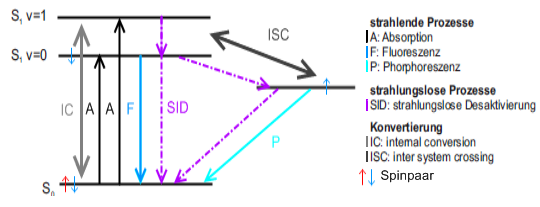
\includegraphics[scale=0.5]{graphics/Jablonski_Termschema}
\caption{Jablonsky-Termschema \cite{[3]} } 
\end{figure}

Die Singulett-Zustände werden dabei als $S_0$ (Grundzustand),$S_1, S_2$...und die Triplett-Zustände als $T_1, T_2$ bezeichnet. Auf einige dieser Vorgänge wird genauer eingegangen.
\subsection{internal conversion}
Dabei handelt es sich um einen Übergang ohne Strahlung zwischen zwei elektronischen Zuständen mit der gleichen Spinmultiplizität. Auf diesen Prozess folgt in Lösung eine Schwingungsrelaxation auf den niedrigsten Schwingungslevel des letzten elektronischen Zustandes. Stösst das angeregte Molekül mit Lösungsmittelmolekülen zusammen, kann die Schwingungsenergie übertragen werden. Wegen des großen Energieunterschiedes ist internal conversion vom $S_1$ in den Grundzustand zwar möglich, aber nicht sehr effektiv. Übergänge $S_2$ $\rightarrow$ $S_1$ findet daher eher statt. Interne Conversion von $S_1$ zu $S_0$ steht in direkter Konkurrenz zu Fluoreszenz und zu intersystem crossing.
\subsection{Fluoreszenz}
Als Fluoreszenz bezeichnet man das Aussenden von Photonen bei der Rückkehr von $S_1$- in den $S_0$-Zustand. Das Fluoreszenzspektrum liegt auf höheren Wellenlängen (niedrigerer Energie) als das Absorptionsspektrum, weil Energie durch Schwingungsrelaxation verlorengeht. In den meisten Fällen überlappt das Absorptionsspektrum teilweise das Fluoreszenzspektrum, was laut der Stokes-Regel nicht sein sollte. Der Abstand (ausgedrückt in Wellenzahlen) zwischen dem ersten Absorptionsband und dem Maximum des Fluoreszenzbandes wird als Stokesshift bezeichnet. Die Emission von Licht und die Anregung sind gleich schnell und betragen ca. 10$^{-15}$s. Angeregte Moleküle verbleiben im $S_1$ Zustand für eine bestimmte Zeit (Picosekunden bis Nanosekunden), bevor sie ein Photon emittieren oder in andere Zustände übergehen. Der beschriebene Prozess ist spontan, kann aber auch unter bestimmten Umständen stimuliert werden.
\subsection{intersystem crossing}
Intersystem crossing ist ein strahlungsloser Übergang zwischen zwei isoenergetischen  Schwingungszuständen, die zu elektronischen Zuständen unterschiedlicher Multiplizität gehören. Ein Beispiel dafür wäre der Übergang von Singulett- in den Triplett-Zustand. Übergänge von Zuständen unterschiedlicher Multiplizität ist zwar verboten, kann aber  über eine Spinbahnkupplung, die groß genug ist, ermöglicht werden. Von den Singulett- und Triplettzuständen hängt es ab, ob Intersystem crossing überhaupt stattfinden kann. Wenn der Übergang $S_0$ $\rightarrow$  $S_1$ ein n$\rightarrow$n* Typ ist, kann intersystem crossing effizient sein. Die Anwesenheit von schweren Atomen begünstigen Spinbahnkupplung und bevorzugen intersystem crossing.

\subsection{Phosphoreszenz}
Bei Raumtemperatur in Lösung ist das strahlungslose Zurückfallen vom Triplettzustand $T_1$ bevorzugt gegenüber dem Zurückfallen mit Strahlung (Phosphoreszenz). Der Übergang $T_1$ $\rightarrow$ $S_0$ ist eigentlich verboten (wegen Spinbahnkupplung aber möglich) und die Strahlungsrate ist sehr niedrig. Nicht nur bei niedriger Temperatur oder in einem starren Medium kann Phosphoreszenz beobachtet werden, sondern es gibt auch Farbstoffe, die bei Raumtemperatur effiziente Phosphoreszenz zeigen. %citation needed%
Wenn die Lebensspanne am Triplettzustand lange genug ist, kann unter diesen Bedingungen Phosphoreszenz in einem Zeitbereich von Sekunden oder sogar Minuten oder länger beobachtet werden. Das Phosphoreszenzspektrum ist auf höheren Wellenlängen angesiedelt als die Fluoreszenzspektrum, weil die Energie vom niedrigsten Schwingungszustand vom Triplettzustand $T_1$ niedriger ist als die vom Singulettzustand $S_1$.

\subsection{thermisch aktivierte verzögerte Fluoreszenz}
Umgekehrtes intersystem crossing $T_1 \rightarrow S_1$ kann auftreten, wenn die Energiedifferenz zwischen $S_1$ und $T_1$ klein ist und die Lebensspanne vom $T_1$-Zustand lang genug ist. Dies geschieht mit derselben spektralen Verteilung wie die normale Fluoreszenz, aber mit einer längeren Halbwertszeitkonstanten, weil die Moleküle im Triplettzustand bleiben, bevor sie zum $S_1$-Zustand emittieren. Diese Fluoreszenzemission ist thermisch aktiviert, d.h mit steigender Temperatur steigt die Effizienz.

\subsection{Triplett-Triplett-Übergang}
Wenn ein Molekül angeregt wurde und den Triplett Zustand $T_1$ erreicht, kann es andere Photonen von verschiedenen Wellenlängen absorbieren, weil Triplett-Triplett-Übergänge erlaubt sind. Diese Übergänge können beobachtet werden, wenn die Menge an Molekülen im Triplett-Zustand groß genug ist. \cite{[4]} %valeur
\subsection{Lumineszenz-Löschung}
Dieser Effekt bezeichnet Vorgänge, die eine Abnahme in der Intensität der Fluoreszenz eines Fluorophors zur Folge haben, ohne dass der Fluorophor zerstört wird. Die Lumineszenzlöschung ist reversibel, d.h beim Entfernen des Quenchers stellt sich die Lumineszenz wieder ein.
\\Beim dynamischen Quenching wird die Energie des angeregten Fluorophors durch den Zusammenstoss mit einem Quenchermolekül auf dieses Quechnermolekül übertragen, wobei die Energie in Wärme übergeht.
\\Beim statischen Quenching bilden Fluorophor und Quenchermolekül einen Komplex, dessen Fluoreszenz verringert ist oder ganz ausbleibt. %cite valeur
\chapter{Sensoren}
\section{Definition}
Als Sensoren werden Messfühler bezeichnet, welche z.B. optische, akustische, elektrische, magnetische oder auch stoffspezifische Signale empfangen und dies in einer verarbeiteten Form weiterleiten. Dabei ist die Reversibilität sehr wichtig.
\\Chemische Sensoren bestehen aus einem Stoffe erkennenden Teil und einem Messwertumwandler, der die Information im zu analysierenden Medium (Gas, Flüssigkeit) in ein elektrisches oder optisches Signal umändert.
\\Biochemische Sensoren enthalten eine biochemische oder biologische Komponente (Enzym, Antikörper, Zelle, Mikroorganismen) in Verbindung mit einem physikalisch-chemischen Messprinzip (Elektroden: Potenziometrie oder Amperometrie, Fluoreszenz u.a.).
\\Den Wechselwirkungsprozessen zwischen Analyt und Sensoren liegen physikalisch-chemische oder biochemische Mechanismen bzw. Prinzipien zugrunde:
\\Physiosorption, van der Waals-Kräfte und Chemisorption, Oberflächen-, Volumen-, Korngrenzen-, Grenzflächen- und Dreiphasen-Reaktionen, Reaktionen mit Käfigverbindungen und spezifische Reaktionen in Biosensoren.
\\Zu den physikalisch-chemischen Grundlagen der Analytik mit Sensoren gehören thermodynamische und kinetische Aspekte, angefangen von der Zustandsfunktion, dem Prinzip der Minimierung der freien Energie bzw. freien Enthalpie (Gibbs'sche Energie), der Berechnung der Zustandssumme, Berechnungen zur heterogenen Katalyse bis hin zur Aufstellung von Energiediagrammen und Funktionen zur Reaktionsgeschwindigkeit.
\\Man unterscheidet unter Verwendung der genannten thermodynamischen und kinetischen Grundlagen drei Arten von Sensorprinzipien: Gleichgewichtssensoren (thermodynamische Gleichgewichte), umsatzratenbestimmende Sensoren (unter kinetischen Fließgleichgewichtsbedingungen) und Einwegsensoren (ohne Reversibilität des Reaktionsprinzipes). \cite{[5]} %schwedt
%Reversibilität ist sehr wichtig, definition eines Sensors
\section{optische Sensoren}
Die Glasfasertechnik spielt bei der Entwicklung optischer Sensoren eine wichtige Rolle. Weil Glasfaserlichtleiter kleine Durchmesser aufweisen, begünstigt dies die Herstellung von Glasfaserlichtleitern, die bei der Konstruktion von in-vivo-Sensoren Anwendung finden. Mit diesen kann man z.B. in Körperflüssigkeiten messen. Der in vivo-pH-Optosensor auf faseroptischer Basis besteht aus einer kleinen Cellulose-Dialyseröhre, in der sich der Indikator Phenolrot (gebunden an Polyacrylamid-Partikel) und etwa 1 \textmu m große Polystyrolkügelchen als Füllung befinden. Die Dialyseröhre ist direkt an ein Lichtleiterpaar aus Kunststoff gekoppelt. Das eingestrahlte Licht wird an den Polystyrol-Kugeln (Indikatorkugeln), die mit Körperflüssigkeit in Kontakt stehen, gestreut und ändern ihr Lichtabsorptionsverhalten in Abhängigkeit vom pH-Wert. Das über die zweite Lichtfaser zurückgestrahlte Licht wird schließlich auf eine Photodiode übertragen. \cite{[5]}
%gibt es auch in Polymer siehe Klimant/Mayr oder A.Mills

\subsection{Faseroptische Sensoren}
Diese Art von Sensoren findet auch Einsatz in Fließsystemen. Durch Remissionsmessung ( Wiederaussendung von einfallenden Wellen oder Teilchen) werden die pH-abhängigen Absorptionsänderungen bestimmt.
Bei Faseroptischen Sensoren in Polymeren wird der Lumophor in Silica-Gel-Kugeln integriert und getrocknet. Dann wird er mit einem Silicon-Prepolymer homogen vermischt, für 12 h bei 40°C ausgehärtet. Das Silkon wird dann in heißes Wasser getaucht um  es zu füllen. Das in den Sensor eindiffundierte Wasser verändert die Polarität in Umgebung des Farbstoffes. Dies führt zu einer kontinuierlichen hypsochromen Verscheibung der Absorption in Abhängigkeit vom Wassergehalt. \cite{[6]} %mills
Beim Ammoniak-Optosensor  wird der Analytstrom vom Indikatorsystem getrennt (durch eine weiße permeable Teflon-Membran) und kann so kontinuierlich gemessen werden. Die Änderung der Farbe, die an der Grenzfläche auftritt, kann ermittelt werden. Die Fluorometrie wird genauso wie die Photometrie in Optosensoren verwendet. Lichtleiter können auch direkt chemisch beschichtet werden. An einem Ende wird der Lichtleiter mit Licht einer Leutdiode durchstrahlt, und wird mittels Photodiode registriert. Beim Durchstrahlen der gassensitiven Beschichtung wird der Grenzwinkel eingehalten, um  eine intern an der Grenzschicht Polymer/Luft zu reflektrieren. Wenn Moleküle des Analyten die Schicht durchwandern setzen sie sich mit der vorhandenen Reagenz. Der intern reflektierte Lichtstrahl wird somit abgeschwächt.\cite{[5]}
%andere Formen planare Optode, imaging mit CCD-Kamera, Nanopartikel
\\Bei planaren Optoden basiert die Messung auf der Verwendung von spezifischen Fluoreszenzfarbstoffen, die kurzfristig mit Licht einer oder mehrerer spezieller Wellenlängen angeregt werden. Der Farbstoff wird in einer Polymermatrix fixiert und auf das untersuchende Medium aufgebracht. Die Messung erfolgt z.B. mit CCD-Kamera außerhalb des Mediums. Damit ist auch nicht-invasive Erfassung möglich. %googlecite
\subsection{optothermische Sensoren}
Neben den oben vorgestellten Sensoren werden auch optothermische (photoakustische) Sensoren eingesetzt. Materie wird mit Licht z.B. im IR-Bereich für $CO_2$ oder $NO_2$ Analysen bestrahlt wird und wenn die IR-Strahlung absorbiert wird, so vergrößert sich das Gasvolumen und dieser Druckanstieg stellt das Messsignal dar. \cite{[5]}
\section{optische Sauerstoffsensoren}
In Wissenschaft und Technik spielt Sauerstoff als Analyt eine wichtige Rolle. Dies kann über optische Sensoren, die nichtinvasiv oder minimal invasiv (invasiv= in Gewebe eindringend) und austauschbar sind, überprüft werden. Sie können leicht verkleinert werden und die Sauerstoffdichte in einem Volumen oder über einer Oberfläche messen. Als UV-Vis Sauerstoffindikatoren werden vor allem luminiszierende Metallkomplexe verwendet, z.B. Ruthenium(II)polypyridyl-Komplexe, Platin(II) und Palladium(II)-Porphyrine oder Iridium(III)-Coumarine. \cite{[6]}
\\Das Messprinzip eines optischen Sauerstoffsensors basiert auf der optischen Messung der Sauerstoffkonzentration. Auf die Spitze eines optischen Kabels wird ein chemischer Film geklebt, der die Phosphoreszenzeigenschaften misst, die von der Sauerstoffkonzentration abhängen. Die Phosphoreszenz ist am Maximum, wenn kein Sauerstoff vorhanden ist. Wenn $O_2$-Moleküle mit dem Film zusammenstossen, löschen sie die Photolumineszenz aus. In einer festgelegten Sauerstoffkonzentration werden bestimmt viele $O_2$-Moleküle mit dem Film zu jeder Zeit zusammenstossen und die Phosphoreszenz-Eigenschaften werden stabil sein.
\\Das Signal-Sauerstoff-Verhältnis ist nicht linear und eine Optode ist am empfindlichsten, wenn die Sauerstoffkonzentration niedrig ist. Das heißt, dass die Empfindlichkeit sinkt, wenn die Sauerstoffkonzentration steigt. Der Optodensensor kann im gesamten Bereich von 0-100$\%$ Sauerstoffsättigung im Wasser arbeiten.
%kann man auch graphisch zeigen; Stern-Volmer-gleichung ist wichtig
\begin{figure}[!htpb]
\centering
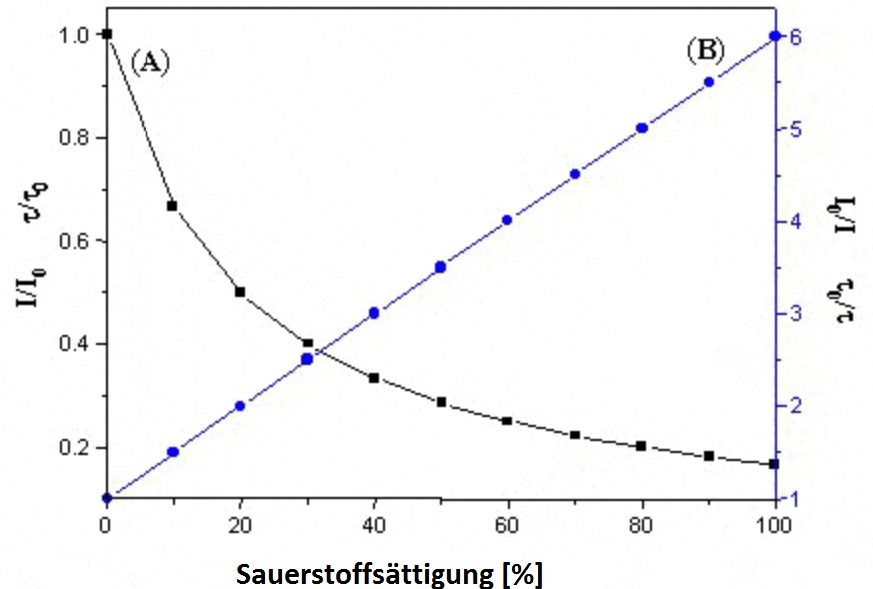
\includegraphics[scale=0.5]{graphics/stern-volmer}
\caption{(A) Lumineszenzabnahme in Gegenwart von Sauerstoff; (B) Stern-Volmer-Plot}

\end{figure}
 Kein Sauerstoff wird verbraucht und deswegen ist der Sensor unempfindlich gegenüber Rührung (diese kann das Signal schneller stabilisieren). Diese Art von Sensor kann für in-situ und Echtzeit- Beobachtung der Sauerstoffproduktion in Wasserabspaltenden Reaktionen benutzt werden. \cite{[7]}
\\Die oben beschriebenen Sauerstoffsensoren haben auch Grenzen. Diese Sensoren können nicht in mehrfachstreuenden und fluoreszierenden Materialien (z.B.Chlorophyll) enthaltenden Medien benutzt werden. UV-Vis Indikatoren sind nicht für Messungen in Unterhautgewebe geeignet, weil es zu hohen Streuverlusten kommt und weil Blut Licht im sichtbaren Bereich absorbiert.
\\Dafür können NIR-Sauerstoff-Indikatoren verwendet werden, die den Vorteil haben, weniger zu streuen, weniger Autofluoreszenz zu haben und das Messungen im Gewebe möglich sind \cite{[6]} %borisov
\subsection{Implantierbare Glukose-Sensoren}
%Prinzip erklären; Gleichung
Das Prinzip dieser Sensoren ist, dass Glukose in Gegenwart von Sauerstoff und Wasser  von dem Enzym Glukose-Oxidase zu Gluconolacton umgewandelt wird und die Abnahme des Sauerstoffs gemessen wird:
\\\ce{Glukose + O2 + H2O ->T[Glukose][oxidase] Gluconolacton + H2O2}
\\Implantierbare Glukose-Sensoren könnten bei der Diabetes-Überwachung helfen und verlassen sich auf Sauerstoffindikatoren als Transduktoren. Sie sollen unter der Haut implantiert werden und vitale Analyten wie Glukose oder Sauerstoff überwachen. Solche "Tattoos" werden über die Haut angeregt und interagieren mit einer Photodiode oder einer CCD-Kamera.  \cite{[6]}
\begin{figure}[htpb]
\centering
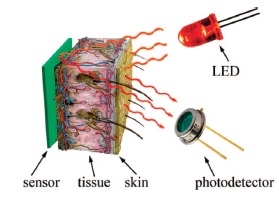
\includegraphics[scale=1]{graphics/Glucose-Sensor}
\caption{Aufbau eines Implantierbaren Glucosesensors}
\end{figure}

\chapter{Porphyrine}
Porphyrine sind organisch-chemische Farbstoffe, die aus 4 Pyrrol-Ringen (Tetrapyrrol) bestehen, die durch vier Methingruppen zyklisch miteinander verbunden sind. Beispiele für Porphyrine sind das Chlorophyll (Farbstoff in Pflanzen) und das Häm in den Proteinen Hämoglobin und den verschiedenen Cytochromen.
\\Sie können als Farbstoff und als Elektronenüberträger dienen.
\section{biologische Bedeutung}
Eine essentielle Rolle spielen Porphyrine im Stoffwechsel der Lebenwesen. Im Gegensatz zu anderen Naturstoffen(Aminosäuren, Kohlenhydrate, Lipide) werden sie nicht als Substrate im Stoffwechsel benutzt, sondern sie finden Anwendung als Katalysatoren oder Coenzyme und sind als solche an der biologischen Oxidation und am Sauerstofftransport beteiligt. Da sie als Farbstoffe aktiv sind, geben sie den Proteinen ihre charakeristische Farbe(Chromoproteine). Porphyrine leiten sich vom Porphin ab, das aber so nicht in der Natur vorkommt.
\begin{figure}[!htpb]
\centering
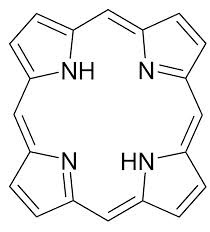
\includegraphics[scale=0.5]{graphics/porphin}
\caption{Porphin: Grundstruktur von Porphyrinen}
\end{figure}
Natürliche Porphyrine sind durch ihre Substituenten charakterisiert. Bei der Biosynthese entstehen zunächst die Porphyrinogenderivate, die einen höheren Sättigungsgrad besitzen und durch Dehydrierung zu Porphinderivaten werden. Eine für ihre biologische Funktion wichtige Eigenschaft ist ihre Neigung zur Chelatbildung von Metallen (Fe, Mg, Zn). Viele Eisen-Porphyrinverbindungen zeigen eine tiefrote Farbe.\cite{[8]}
\begin{figure}
\centering
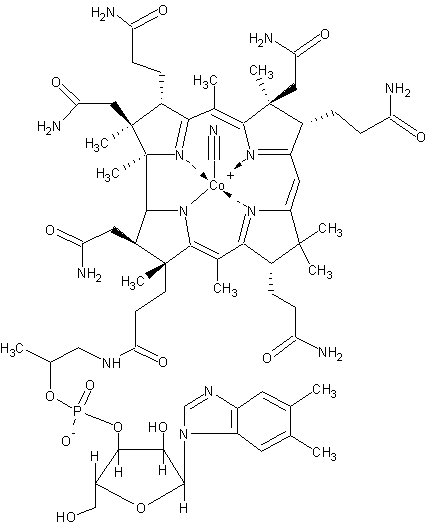
\includegraphics[scale=0.5]{graphics/Vitamin_B12}
\caption{Vitamin B 12}
\end{figure}
\begin{figure}[!htpb]
\centering
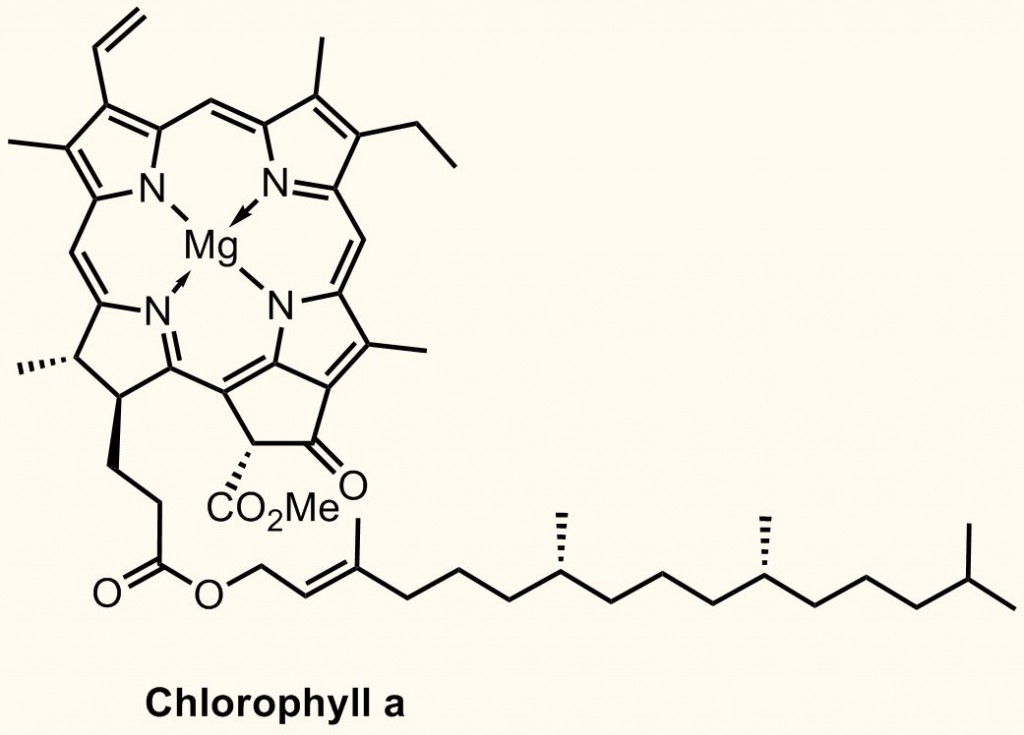
\includegraphics[scale=0.5]{graphics/Chlorophylla}
\caption{Chlorophyll A}
\end{figure}

\begin{figure}[!htpb]
\centering
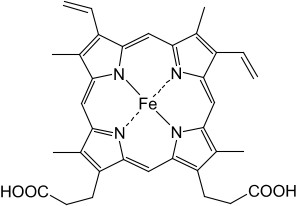
\includegraphics[scale=0.5]{graphics/haem3}
\end{figure}

\section{Arylethinylporphyrine}
\begin{figure}[!htpb]
\centering
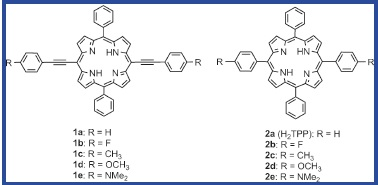
\includegraphics[scale=1]{graphics/arylethinylporphyrin}
\caption{Arylethinylporphyrine}
\end{figure}
Die Ethninyl-Funktionalität verlängern das konjugierte $\pi$-System des Porphyrins und entfernt die sterische Barriere zwischen Phenylgruppe und dem Porphyrin-Makrozyklus und erweitert die Konjugation über die Achsen des Moleküls. Solche Modifikationen führen zu Rotverschiebungen der B- und Q-Regionen. Die erweiterte Konjugation erleichtert die elektronische Kommunikation zwischen Porphyrin und den funktionellen Gruppen.
\\Arylethinyl Porphyrine werden in verschiedenen Bereichen, z.B. künstliche photosynthetische Systeme oder nichtlineare optische Materialien angewendet. Während Metall (Zn, Cu, Ni, Fe) Arylethinylporphyrine weit erforscht sind, gibt es nur wenige Studien zu metallfreien Arylethinylporphyrinen. Unter den richtigen Bedingungen, weisen manche metallfreie Porphyrine Hyperporphyrin-Spektren auf, die nicht mit den Vier-Orbital-Porphyrin-Model beschrieben werden können. Stattdessen entsteht ein Charge-Transfer-Übergang zwischen Substituent und Porphyrin-Ring. Diese Übergänge entstehen bei niedrigerer Energie und mit höherer Intensität als normale Porphyrin Q-Band Übergänge. 
\\Protonierung an den zentralen Stickstoff-Atomen resultiert in nichtplanare Verzerrungen im Porphyrin-Makrozyklus und bewirkt eine Veränderung in den photophysikalischen Eigenschaften wie rotverschobene Absorptions-Spektren, größeren Stokes-Shift, größere Fluoreszenzlinien und verkürzte Anregungs-Lebensspanne. \cite{[9]}
\section{$\pi$-erweiterte Porphyrine}
Porphyrine, die über Verschmelzung mit externen aromatischen Ringen erweitert wurden, besitzen rot-verschobene Absorptionsbanden und starke Lumineszenz bei Raumtemperatur. Die einfachsten Porphyrine in dieser Gruppe, meso-tetraaryltetrabenzoporphyrine wurden schon in biomedizinischen und nichtlinearen optischen Anwendungen benutzt. Tetranaphtoporphyrine wurden nur wenig studiert. Die Erweiterung auf Naphtalo am Pyrrolring führt zu einer Reihe von isomerischen Tetranaphthaloporphyrinen. Tetra[2,3]naphthaloporphyrine (TNP) und meso-tetraaryltetra[2,3]-naphthaloporphyrine (Ar$_4$TNP) sind höher symmetrisch und haben stärkere spektrale Übergänge.
\begin{figure}[!htbp]
\centering
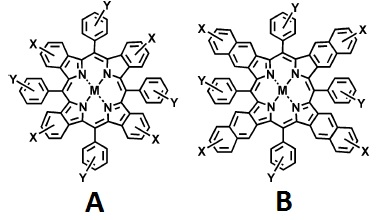
\includegraphics[scale=1]{graphics/MAr4TBP}
\caption{(A) tetraaryltetrabenzoporphyrin und (B) tetranaphtotetrabenzoporphyrin}
\end{figure}
TNPs können durch die Retro-Diels-Alder Reaktion (Umkehrung der Diels-Alder-Reaktion, kann durch Energiezufuhr oder Säuren herbeigeführt werden) hergestellt werden. Diese Methode kann aber keine Substituenten in den aromatischen Ring einbinden.
\\Eine andere Methode wäre eine oxidative Aromatisierung vom Porphyrinen mit nichtaromatischen Cyclohexen-Ringen. Mit dieser Methode können polyfunktionialisierte Ar$_4$TBPs mit guten Ausbeuten synthetisiert werden, z.B. tetra[1,2]naphthaloporphyrine, mono[1,2] und di[1,2]naphtaloporphyrine und mono[2,3]naphthaloporphyrine. \cite{[10]}
\begin{figure}[!htbp]
\centering
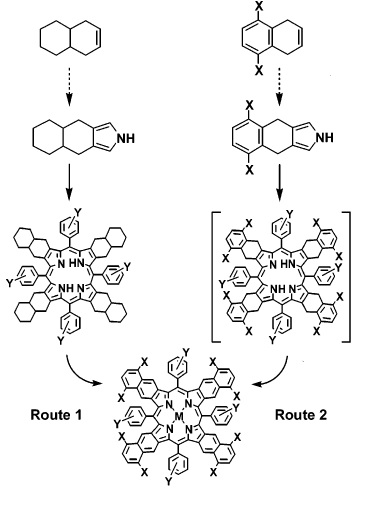
\includegraphics[scale=0.5]{graphics/oxidative_Aromatisierung}
\caption{oxidative Aromatisierung}
\end{figure}
Eine dritte Methode wäre die Template-Synthese
\subsection{meso-meso verknüpfte Porphyrine}
\begin{figure}[!htbp]
\centering
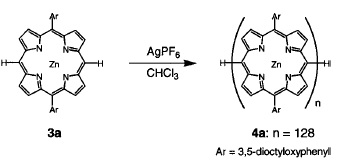
\includegraphics[scale=1]{graphics/meso-meso-fused}
\caption{Synthese von meso-meso-verknüpften Porphyrinen}
\end{figure}
Meso-meso-konjugierte Porphyrine wurden mittels Ag-unterstützten meso-meso-Kuppeln von 5,15-diaryl-substituierten Zn(II)-Porphyrinen zu bis zu 128-teiligen Porphyrinen verknüpft. Diese sollte eines der längsten von Menschen hergestellten Molekülen überhaupt sein. Dieses 128mer ist in organischer Lösemittel löslich. Mittels Gel-Permeations-Chromatographie konnten diese sehr langen Moleküle getrennt werden.
\cite{[11]}
\subsection{direkt verknüpfte Diporphyrine}
\begin{figure}[htpb]
\centering
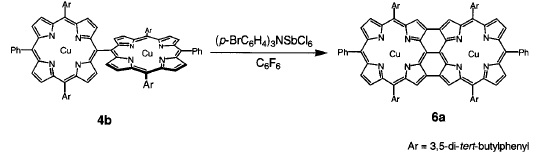
\includegraphics[scale=1]{graphics/diporphyrins}
\caption{Synthese von direkt-verknüpften Diporphyrinen}
\end{figure}
Zwei Porphyrin Ringe können verknüpft werden um eine coplanare Strukur zu bilden. Diese zeigen eine gepackte orthogonale Kristallstruktur, bei der die 3,5-di-tert-butylphenyl-Gruppe zum Cu(II)-diporphyrin zeigt. Es wird so zu einem unendlichen Netzwerk mit mehrern CH/$\pi$ -Wechselwirkungen.
\\Für 6a erkennt man ein Q-Band bei 994 nm (nach rot-verschoben).\cite{[11]}



\chapter{Schollreaktion}
Die Scholl Reaktion ist eine Kupplungsreaktion, bei der zwei Arenmoleküle unter Einfluss eine Lewis-Säure und einer Protonensäure miteinander reagieren. Entwickelt wurde die Methode vom Schweizer Chemiker Roland Heinrich Scholl (1865-1945).
Diese Kondensation kann sowohl intermolekular als auch intramolekular verlaufen. Zum Einsatz kommen Lewis Säuren wir $AlCl_3$ oder auch $MoCl_5$. In der Vergangenheit wurde die Reaktion eher wenig eingesetzt (hohe Umsatztemperaturen, geringe Ausbeuten, stark saure Katalysatoren, viele Nebenprodukte). Aber gerade ihr Einsatz in Kaskadenreaktionen, mit denen man komplexe aromatische Kohlenwasserstoffe oder Graphenstrukturen herstellen kann, machte sie wieder interessant. \cite{[12]}
\section{mögliche Mechanismen der Schollreaktion}
In der Schollreaktion wird die oxidative Aryl-Aryl Kupplungsreaktion von Übergangsmetall-Halogenen beeinflusst. Diese dienen als Lewis-Säure und als Oxidans. Zwei mögliche Mechanismen der Schollreaktion wurden von Nenitzescu und Balaban vorgeschlagen. %ref [13]?
\begin{figure}[!htpb]
\centering
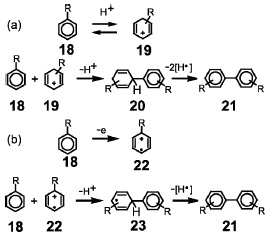
\includegraphics[scale=1]{graphics/Schollreactionmechanismen}
\caption{Menchanismen der Scholl-Reaktion:(a) Arenium-Kation Mechanismus; (b) Radikal-Kation-Mechanismus}
\end{figure}
\\Im Arenium-Kation-Mechanismus wird ein aromatisches Molekül protoniert und der resultierende elektrophilische $\sigma$ Komplex reagiert mit einem anderen aromatischen Kern um einen neue Kohlenstoff-Kohlenstoff-Bindung zu knüpfen. Deprotonierung ergibt das Zwischenprodukt und Dehydrogenierung erzeugt Aromatizität.
\\Im Radikal-Kationen-Mechanismus wird zuerst ein radikales Kation bei einer Ein-Elektronen-Oxidation des Startmaterials gebildet. Dann wird eine C-C-Verknüpfung mit einer aromatischen Gruppe geformt. Deprotonierung und der Verlust eines Wasserstoff-Atoms folgen. Ein arylisch radikalisches Kation wird unter oxidierenden Bedingungen wird zuerst gebildet. Wenn PAHs mit Lewis Säure oder konzentrierte Schwefelsäure behandelt werden, ergeben sich paramagnetischen Lösungen. Deshalb könnten radikale Kationen bei der Schollreaktion entstehen.\cite{[13]}
\section{oxidative Kupplung mit MoCl$_5$}
$MoCl_5$ ist ein schwarzer polymorpher kristalliner Feststoff, der luft- und feuchtigkeitsempfindlich ist und deshalb in inerter Atmosphäre aufbewahrt wird. Das koordinativ ungesättigte $MoCl_5$ ist essentiell für elektrophile Anwendungen. Chlorierte Lösungsmittel, wie Dichlormethan, werden als Reaktionsmedium empfohlen.
\\Bei der Herstellung von hexa-peri-hexabenzocoronen aus hexaphenyl-benzen liefert die Zugabe von $MoCl_5$ die besten Resultate. Diese Reaktion wird später näher erklärt.
Bei der oxidativen Zyklisierung von ortho-terphenylen mit $MoCl_5$ ist das Substitutionsmuster am wichtigsten.  Zumindest eine Donorfunktion soll para zum neu geformten Band stehen, weil sonst kein Produkt entsteht. \cite{14}
\begin{figure}[htpb!]
\centering
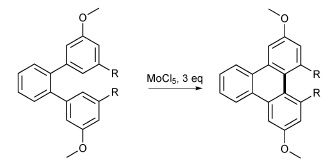
\includegraphics[scale=0.5]{graphics/Scholltriterpene}
\caption{Schollreaktion zu Triphenylen}
\end{figure}

\section{Herstellung von polycyclischen Kohlenwasserstoffen}
\begin{figure}[htpb!]
\centering
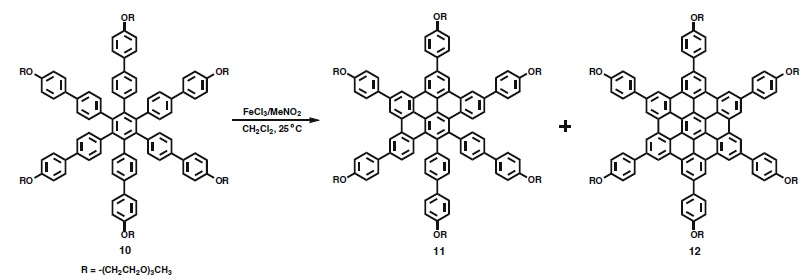
\includegraphics[scale=0.8]{graphics/Schollreactionhbc}
\caption{Synthese von hexaphenyl-1/2HBC und hexaphenyl HBC }
\end{figure}
Hexa peri-hexabenzocoronen(HBC) sind eine Klasse von Polycyclischen Kohlenwasserstoffen, die man als scheibenförmige Strukturen beschreiben kann.  Aus Hexaphenylbenzen kann man mittels Scholl-Reaktion unter Verwendung von $CuCl_2$/$AlCl_3$/$CS_2$ oder $FeCl_3$/$CH_3NO_2$ HBC-Moleküle herstellen. Die Aryl-Aryl dehydrogenische Kupplungsreaktion erfolgt in getrennten Schritten intramolekular mit vier neuen Kohlenstoff-Kohlenstoff-Bindungen in Ausbeute von 10\%. Das ist die einzige isolierte Intermediat einer Schollkondensation eines Hexaphenylbenzen-Vorläufers. Zwei teilweise fusionierte Reaktionsmediate wurden durch Schollkondensation aus einer Kohlenstoff-Oligophenyl-Vorgänger hergestellt. Sterische Hinderung und die Stabilität des Radikalkations bevorzugen diese Formation. Aus pyrimidinhältigen Edukten kann kein HBC hergestellt werden, weil der metallische Katalysator möglicherweise mit dem Substrat reagiert und die Schollreaktion am halben Weg eliminiert. So konnte kein HBC aus einem pyrimidinhältigen Edukt hergestellt werden. Nur richtig designete Hexaphenylbenzen-Vorgänger können eine Schollkondensation eingehen um alkoxy-Substituierte HBCs herzustellen. \cite{[15]}


\part{Praktischer Teil}
\chapter{Durchführung}
\section{5-(pentafluorphenyl)bis(phenylpropinyl)porphyrin}
\subsection{1.Stufe: 5-(Pentafluorophenyl)dipyrromethan}
In einen 50 mL 2-Halskolben werden 25 mL (361,45 mmol) Pyrrol vorgelegt, 2,69 g (13,55 mmol) Pentafluorobenzaldehyd beigemengt und 15 min unter Argonfluss entgast. Mittels Pipette wird 105 \textmu L (1,36 mmol) Trifluoressigsäure zugefügt und 5 min bei Raumtemperatur unter Argonfluss gerührt. Dann wird mit 1 mL 1 M NaOH-Lösung gequencht (pH-Wert überprüfen!) und die Lösung mit 100 mL Ethylacetat in einen Schütteltrichter überführt. 4 mal wird mit jeweils 50 mL Wasser (ein paar Tropfen NaCL-Lösung werden zugefügt) extrahiert. Die organische Phase wird über Na$_2$SO$_4$ getrocknet und mit Filterpapier abfiltriert. Überprüfung mittels DC. Das Lösungsmittel wird am Rotavapor abrotiert und bei Vollvakuum getrocknet. Aufnahme eines NMR-Spektrums zur Reinheitsüberprüfung. Die Aufreinigung erfolgt mittels Kieselgelchromatographiesäule. Die Reinheitskontrolle erfolgt mittels DC. Die Fraktionen mit Produkt werden einrotiert und ein NMR angefertigt. Mittels Ausschütteln mit 40\% iger Ethanol-Lösung (3x 20mL) wird das restliche Pyrrol entfernt. Der Kolben wird im Vakuumtrockenschrank über Nacht getrocknet.
%H-NMR


\subsection{2.Stufe: bis(PF$_5$)bis(PhenylPropinyl)porphyrin}

In einen gekühlten trockenen 500 mL 2-Halskolben mit Argonzufluss werden 515 mg 5-(Pentaluorophenyl)dipyrromethan (1,65 mmol) eingewogen und in 250 mL $CH_2Cl_2$ gelöst. Dann werden 202 \textmu L Phenylpropinyl (1,65 mmol, 215 mg) hinzugefügt. Die Lösung wird 10 min im gekühlten Ölbad gerührt. Das Ölbad wird danach entfernt und das Gefäß mit Alufolie umwickelt und 120 \textmu L $BF_3C_4H_8O$ (0,99 mmol) hinzugefügt und 4 h rühren lassen. Danach werden 800 mg DDQ (3,30 mmol, 2 Äquivalente) hinzugefügt und über Nacht gerührt.
\\ Am nächsten Tag gibt man 1 mL Triethylamin hinzu und rührt. Dann wird das Lösemittel abrotiert und der Kolben im Vollvakuum getrocknet. Reaktionskontrolle mittels DC und Spektrometer ergibt, dass sich kein Produkt gebildet hat, da keine typische Absorption des Porphyrins im Spektrum erkennbar ist.

\section{tetra(propinyl)tetra(3,4 diethylpyrrol)}

In einen 500 mL Zweihalskolben mit Stickstoffzufluss und Kühlbad werden in ca. 400 mL Dichlormethan bei -40°C (Aceton/Stickstoff) 490 \textmu L Phenylpropinyl und 492 mg 3,4-diethylpyroll (4mmol, 1 Äqu.)gegeben und die Apparatur mit Alufolie umwickelt. Nach ca. 0,5 h werden 160 \textmu L BF$_3*OEt_2$ hinzugegeben. Nach 4 h lässt man auf Raumtemperatur abkühlen. Zur Reaktionskontrolle wird ein UV-vis-Spektrum aufgenommen. Da nach Zugabe von 908 mg DDQ (4 mmol) kein typsches Absorptionsspektrum eines Porphyrins erkennbar ist, wird die Reaktion abgebrochen.


\section{tetra(methylphenyl)TBP}
\subsection{1.Stufe: Zinktolylacetat}

2,50 g Tolylessigsäure (16,7 mmol, 2 Äqu.) werden mit 680 mg Zinkoxid (8,35 mmol, 1 Äqu.) vermischt und mit 40 ml EtOH und 20 mL H$_2$O bei 80°C 14 min gerührt. Das Lösungsmittel wird abrotiert und das Produkt bei 70°C und Vollvakuum getrocknet.

\subsection{2.Stufe: Zn-tetra(methylphenyl)TBP}

In einem Becherglas werden 3,84 g 1,2-dicyanobenzene (30 mmol, 4 Äqu.), 4,50 g Tolylessigsäure (30 mmol, 4 Äqu.) und 2,75 g Zinktolylacetat (7,5 mmol, 1 Äqu.) eingewogen und in einem Mörser mittels Pistill vermischt. Die Mischung wird in 15 Supelco Vials aufgeteilt. Die Vials werden im Heizblock auf 280$\circ$C aufgeheizt und für 10 min erhitzt. Die dunkelgrüne Lösung wird abgekühlt. Die Vials werden mit Aceton aufgefüllt und 10 min im Ultraschallbad erwärmt. Dann werden  die Lösungen in einem Becherglas zusammengeschüttet. Eine 1000 mL Lösung bestehend aus 3 Teilen EtOH und 2 Teilen und jeweils 25 mL NaHCO$_3$ und NaCl wird vorbereitet und die Porphyrin-Lösung langsam hinzugegeben (wird gefällt). Der grüne Feststoff wird abfiltriert. Der Vorgang (in Aceton lösen, Ausfällung) wird wiederholt und der Feststoff über Nacht getrocknet.
\\Der Farbstoff wird in Aceton gelöst und eine Säulenchromatographie (Säulenmaterial: Al$_2O_3$) durchgeführt. Der Farbstoff wird mit Cyclohexan und Dichlormethan eluiert. Die Fraktionen, die den Farbstoff enthalten, werden am Rotavapor einrotiert, 2 mal mit Hexan nachgewaschen, 1x mit  Dichlormethan extrahiert und der grüne Farbstoff im Trockenschrank getrocknet.

\subsection{3.Stufe: Demetallierung zu tetra(tolyl)tetrabenzoporphyrin}
0,400 g Zn-tetra(methylphenyl)tetrabenzoporphyrin werden in 200 mL DCM gelöst und 10 min gerührt. Die Lösung wird in einen Schütteltrichter transferiert. Dann wird mit konzentrierter Salzsäure (2x 100 mL), 3x mit jeweils 100 mL destillierten Wasser und zweimal mit 150 mL gesättigter NaHCO$_3$-Lösung extrahiert. Die organische Phase wird über Na$_2$SO$_4$ getrocknet, abfiltriert und das Lösungsmittel mittels Rotavapor entfernt. Das Produkt wird über Nacht bei 60°C getrocknet. Da das Produkt  schlecht lösbar ist, (als Farbstoff ungeeignet), wird hier die Reaktion abgebrochen.

\section{Pt(II)-mono(O-Ethylphenyl)-tris(fluorophenyl)tetrabenzoporphyrin}
\subsection{1.Stufe: Zn-mono(O-Ethylphenyl)-tris(fluorophenyl)tetrabenzoporphyrin}
5,13 g Dicyanobenzene (40 mmol, 4 Äqu.), 2,70 g 4-Ethoxyphenylessigsäure (15 mmol, 1,5 Äqu.),3,85 g 4-Fluorphenylessigsäure (25 mmol, 2,5 Äqu.) und 3,71 g ZnC$_16$H$_12$F$_2$O$_4$ (10 mmol, 1 Äqu.) werden miteinander vermischt und in 22 Supelco-Vials aufgeteilt. Diese werden bei 280$\circ$C für 10 min erhitzt. Nach Abkühlen des Heizblocks werden die Vials mit Aceton aufgefüllt und in ein Becherglas überführt (unlösliche Bestandteile werden mittels Ultraschallbad gelöst). Der Farbstoff wird in 1200 mL (3 Teile EtOH, 2 Teile Wasser, gesättigte NaHCO$_3$-Lösung) ausgefällt und dann abfiltriert. Das Filtrat wird über Nacht in den Trockenschrank gestellt. Die Aufreinigung erfolgt mittels Säulenchromatographie (Säulenmaterial: Al$_2$O$_3$). Die geeigneten Fraktionen werden einrotiert. Der Feststoff wird in Dichlormethan gelöst und in Cyclohexan ausgefällt, abfiltriert und im Vakuumtrockenschrank getrocknet.


\subsection{2.Stufe: Demetallierung zu monoOEttriFPhenTBP}
Das Produkt wird in Dichlormethan gelöst und eine Demetallierung durchgeführt. Die Lösung wird 2 mal mit 36\% Salzsäure und dreimal mit Wasser extrahiert. Nach Extraktion mit gesättigter NaHCO$_3$-Lösung und Wasser wird die organische Phase über Na$_2$SO$_4$ getrocknet und abfiltriert. Das Lösungsmittel wird am Rotavapor abgezogen.

\subsection{3.Stufe: Platinierung}
0,5 mmol (ca. 450 mg, 1 Äqu.) des demetallierten Komplexes werden in einem Rundkolben in 200 mL Trimethylbenzen gelöst und mit 250 mg cis-Platin (1 mmol, 2 Äqu.) vermengt und auf 170°C erhitzt. Reaktionskontrolle erfolgt über Aufnahme von Spektren. Nach 1 Stunde wird 150 mg Platinkomplex hinzugegeben. Nach 1 weiteren Stunde wird die Reaktion abgebrochen und auf Raumtemperatur abgekühlt. Dann wird das Lösungsmittel abgezogen. Die Reinigung erfolgt mittels Säulenchromatographie( Säulematerial: Al$_2$O$_3$, eluiert wird mit Cyclohexan und Dichlormethan). Die Trennung des Produktes von seinen Isomeren (di- und nicht-substituierte Nebenprodukte) konnte nicht erreicht werden.

\section{Verbrückung von Pt(II)tertbutylbenzoporphyrin mittels Schollreaktion}
In einen Rundkolben werden 15 mg Tertbutylbenzoporphyrin und 120 mg AlCl$_3$ in 15 mL Dichlorbenzen gelöst. Der Kolben wird 5 min im Ultraschallbad erhitzt. Dann wird im Ölbad auf 170 $\circ$C erwärmt und 15 min gekocht. Danach werden 50 mg MoCl$_5$ zugegeben und 3 min weiter erhitzt. Danach wird die Reaktion abgekühlt. Die Lösung wird in 150 mL DCM und 4 mL Et$_3$N gegeben und zentrifugiert. Das Sediment wird 2 mal nachgewaschen. Dann wird die Lösung dreimal mit NaCl-Lösung extrahiert. Die wässrige Lösung wird einmal mit DCM nachgewaschen.  Die vereinigten organischen Phasen werden über Na$_2$SO$_4$ getrocknet. Die Reaktionskontrolle erfolgt über ein DC( Laufmittel: CH:DCM=1:1). Zur Aufreinigung wird eine Säulenchromatographie gemacht. Das fertige Produkt wird in Toluol gelöst und ein Fluoreszenzpektrum aufgenommen. Die Reaktionskontrolle erfolgte über das UV-vis-Spektrum. Durch Vderscheibung der Peaks nach rechts konnte das Produkt nachgewiesen werden.

\section{Verbrückung von PttBumonoAzaTBP mittels Scholl Reaktion}
2mg PtAzaporphyrin werden mit 15 mg $AlCl_3$ und 5 mg $MoCl_5$ in 2 mL Dichlorbenzen gelöst und im Heizblock in einem Vial bei 170$\circ$C 15 min erhitzt.Nach Abkühlen der Lösung wird diese in 30 mL Dichlormethan und 5 mL Triethylamin gegeben und abfiltriert. Dann wird 3x mit 50mL $H_2O$ extrahiert, über $Na_2SO_4$ getrocknet, abfiltriert. Danach wird das Dichlormethan abgedampft und ein Fluoreszenzspektrum aufgenommen:

\chapter{Ergebnisse und Diskussion}
\section{5-(Pentafluorophenyl)dipyrromethan}
\begin{figure}[!htpb]
\centering
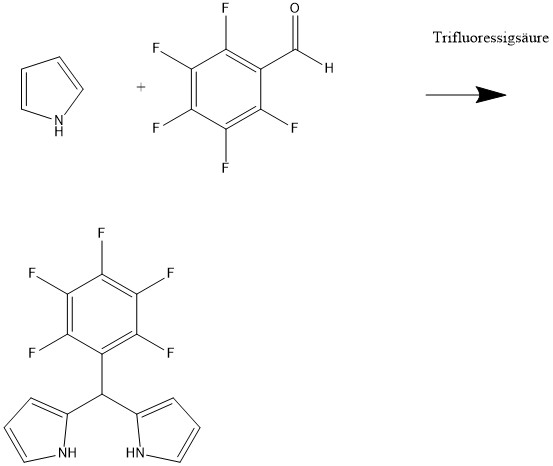
\includegraphics[scale=0.5]{graphics/5-(Pentafluorphenyl)dipyrromethan}
\caption{Synthese von 5-(Pentafluorophenyl)dipyrromethan}
\end{figure}
Das Produkt dient als Vorlage für einen Porphyrinkomplex. Die Reaktion lief wie erwartet, jedoch war die Aufreinigung etwas aufwendiger. Das Pyridin konnte nur mittels Extraktion entfernt werden und nicht mittels Chromatographiesäule. Das Spektrum (siehe \ref{5pfdpmnmr1}) wurde direkt nach der Reaktion ohne Aufreinigung aufgenommen. Die Peaks für die Pyrrolverunreinigungen sind bei 6,82; 6,26 und 5,8. Die restlichen Peaks zeigen den Pyrrolring. Das Lösungsmittelsignal ist bei ca. 7,3. Das Verhältnis von Pyrrol zu Produkt liegt bei 50\%. Nach einmaliger Aufreinigung mittels Kieselgelsäure ist noch immer  viel Pyrrol vorhanden (ca.30\%) Beim Extrahieren mit 40\% Ethanol-Lösung konnte das Pyrrol fast vollständig entfernt werden.
\section{di-(pentafluoro)-di-(Phenyl-Propinyl)porphyrin}
\begin{figure}[!htpb]
\centering
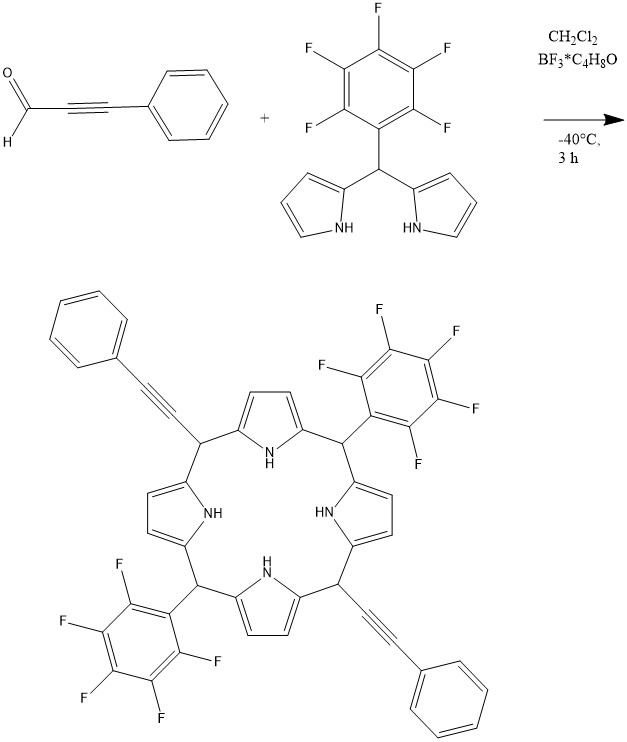
\includegraphics[scale=0.5]{graphics/bis(pentafluorphenyl)-bis(phenylpropinyl)porphyrin}
\caption{Synthese von di-(pentafluoro-die-(Phenylpropinyl)porphyrin}
\end{figure}
Der Komplex wurde laut Paper \cite{16} %%blabla 
mit leicht geänderten Seitenketten hergestellt, da die Synthese recht interessant ausgesehen hatte und der Porphyrinkomplex möglicherweise gute Fluoreszenzeigenschaften gehabt hätte. Im Absorptionsspektrum konnte das Produkt nur gering (leichter Bogen bei 650 nm) bis gar nicht nachgewiesen werden.
Die Lösung blieb nach der Reaktion schwarz und es war kein Porphyrin im Spektrum zu sehen. Vermutlich ist das Produkt während der Reaktion zerfallen oder es konnte nicht stabilisiert werden.

\section{tetra(propinyl)tetra(3,4 diethylpyrrol)}
\begin{figure}[!htpb]
\centering
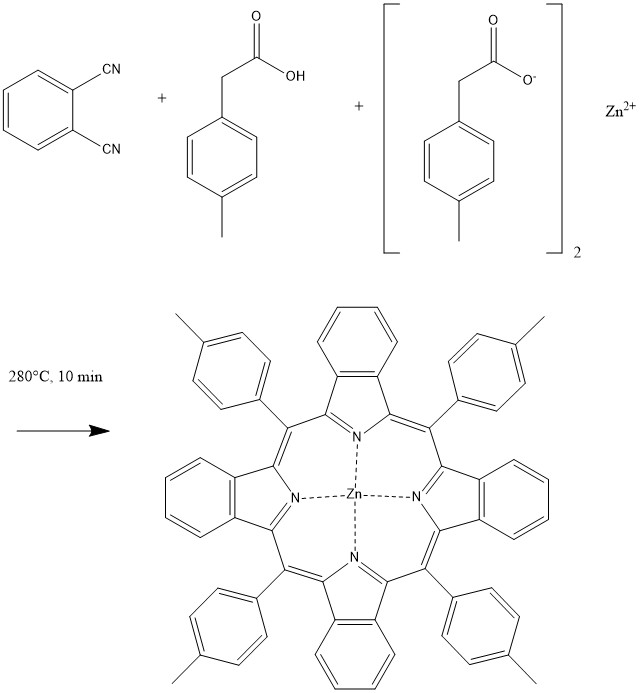
\includegraphics[scale=0.5]{graphics/tetrakis(methylphenyl)tetrakis(phenylpyrrolporphyrin}
\end{figure}
Diese Reaktion wurde genau nach Anleitung \cite{[16]} gemacht, mit den gleichen Edukten und Produkten. Jedoch konnte nur wenig Prophyrin nachgewiesen werden. Das Spektrum hat Bögen. Die Lösung war nach der Reaktion schwarz und hatte keine charakteristische Farbe eines Porphyrins. Das Produkt ist zerfallen oder konnte gar nicht hergestellt werden.
\section{Zinktolylacetat}
\begin{figure}[!htpb]
\centering
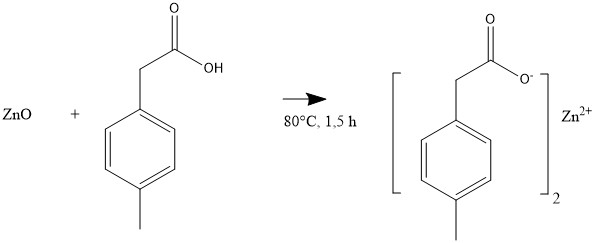
\includegraphics[scale=0.5]{graphics/zinktolylacetat}
\end{figure}
Das zweifach geladene Zinktolylacetat wurde zum Einbau von Zink in den Komplex hergestellt.
Das Produkt und das Edukt wurden anschließend für die Herstellung eines Porphyrinringes verwendet. Da die Reaktion vergleichsweise einfach war und hohe Ausbeuten erwartet werden, wurde auf eine Reaktionskontrolle verzichtet. 
\section{Zn-tetra(tolyl)tetrabenzoporphyrin}
\begin{figure}[!htpb]
\centering
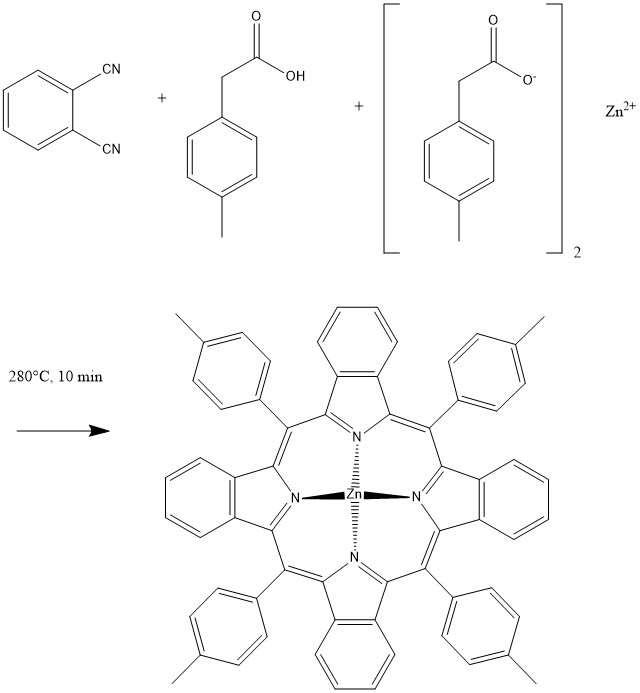
\includegraphics[scale=0.5]{graphics/ZnTtolyltbp}
\end{figure}
Der Zink-Porphyrinkomplex wurde wegen möglicher guter Fluoreszenzeigenschaften hergestellt. Die Methylgruppe am Benzolring soll zusätzlich Löslichkeit bringen, da Porphyrine wegen ihrer Größe grundsätzlich schlechter löslich sind. 
Im NMR-Spektrum erkennt man Peaks bei 8,25 (Multiplett), 7,6(Multiplett); 7,5 (m); 7,25(m); 7,2 (Singlett) und 2,5. Das Spektrum wurde in $C_6D_6$ aufgenommen (Peak bei 7,2). Das Produkt ist ausreichend vorhanden.
\newpage
\section{tetra(tolyltetrabenzoporphyrin}
\begin{figure}[!htpb]
\centering
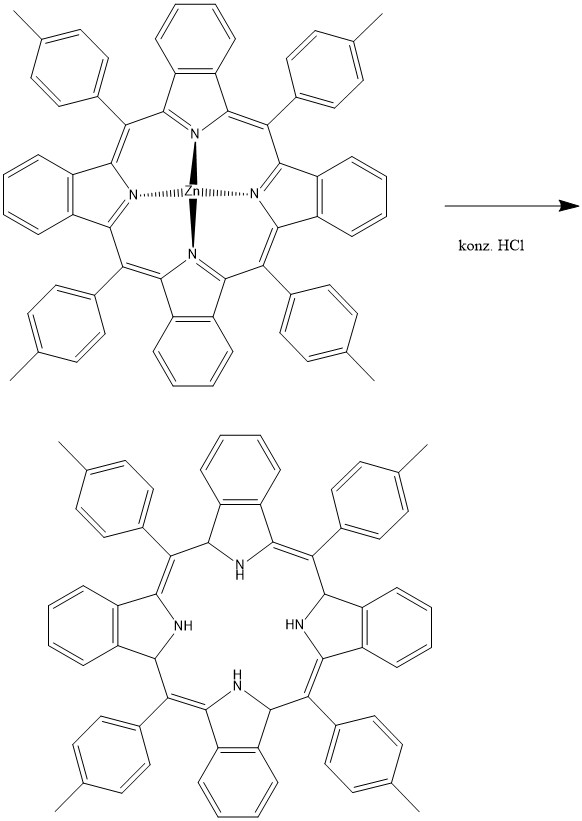
\includegraphics[scale=0.5]{graphics/demetoftetramehtphen}
\end{figure}
Die Demetallierung wurde durchgeführt um Zink aus dem Komplex zu entfernen und später Platin einzuführen. Nach der Reaktion war jedoch kaum Produkt im Spektrum zu erkennen. Die Massenberechnung nach Lambert-Beer'schen Gesetz ($A=\epsilon*c*d$) ergab nur 2,4 mg Produkt. Das kann daran liegen, dass das Produkt beim Filtrieren am Filterpapier hängengeblieben ist, weil es schwer löslich war. Daher ist es als Farbstoff ungeeignet und die Reaktion wurde abgebrochen.
\newpage
\section{ZnmonoOEttriFPhenTBP}
\begin{figure}[!htpb]
\centering
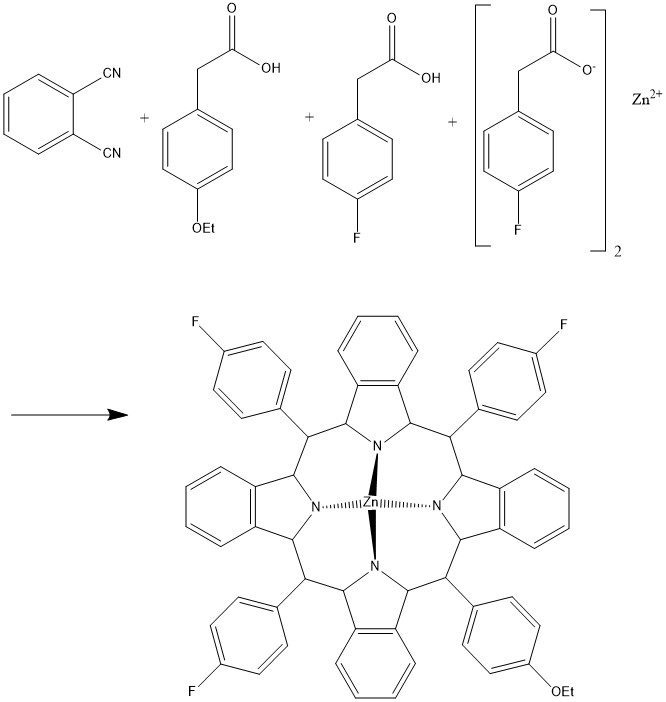
\includegraphics[scale=0.5]{graphics/Zn(ethoxyphenyl)tris(fluorophenyl)tetrakis(phenylpyrrol)porphyrin}
\end{figure}
Ziel dieser Reaktion war es, einen Porphyrinkomplex mit einer Phenyl-O-Ethyl-Gruppen und drei Fluor-Phenyl-Gruppen zu synthetisieren.  Das H-NMR-Spektrum wurde in $CDCl_3$ aufgenommen (Peak bei 7,3). Man erkennt mehrere Singlett-Peaks (8,4;8,2;7,5;4,4; und 1,7) und ein Multiplett bei 7,4. Laut Spektrum haben sich eher Porphyrine mit 2 Phenyl-O-Ethyl-Gruppen und 2 Fluor-Phenylgruppem gebildet, was mit der Abmischung der Edukte zusammenhängen könnte.

\section{mono(O-ethylphenyl)tris(fluorophenyl)tetrabenzoporphyrin}
\begin{figure}[!htpb]
\centering
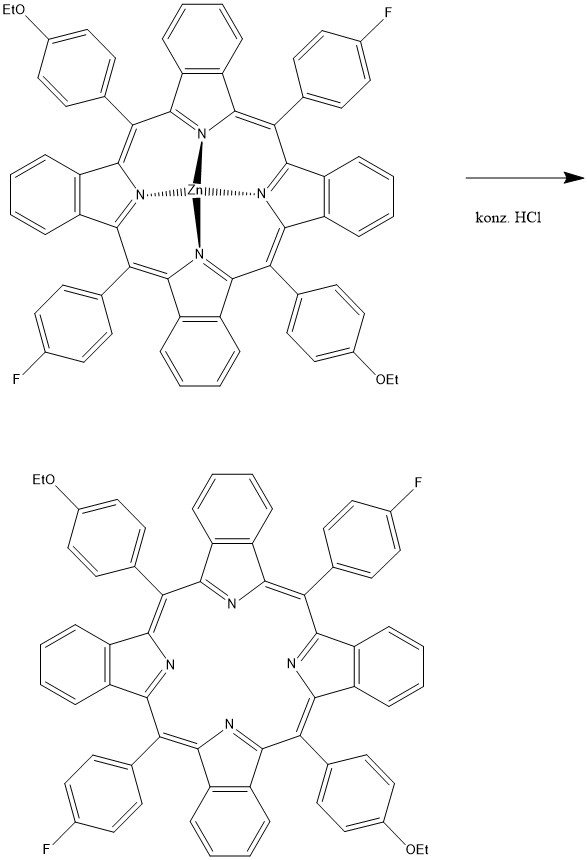
\includegraphics[scale=0.5]{graphics/entmetZnmonoettrifphenTBP}
\end{figure}
Zur Entfernung des Zink als Zentralatom und um dann später eine Platinierung durchzuführen, wurde die Demetallierung mit konzentrierter Salzsäure durchgeführt. Eine Reaktionskontrolle erfolgte nicht.


\section{PtmonoOEttrFPhenTBP}
\begin{figure}[!htpb]
\centering
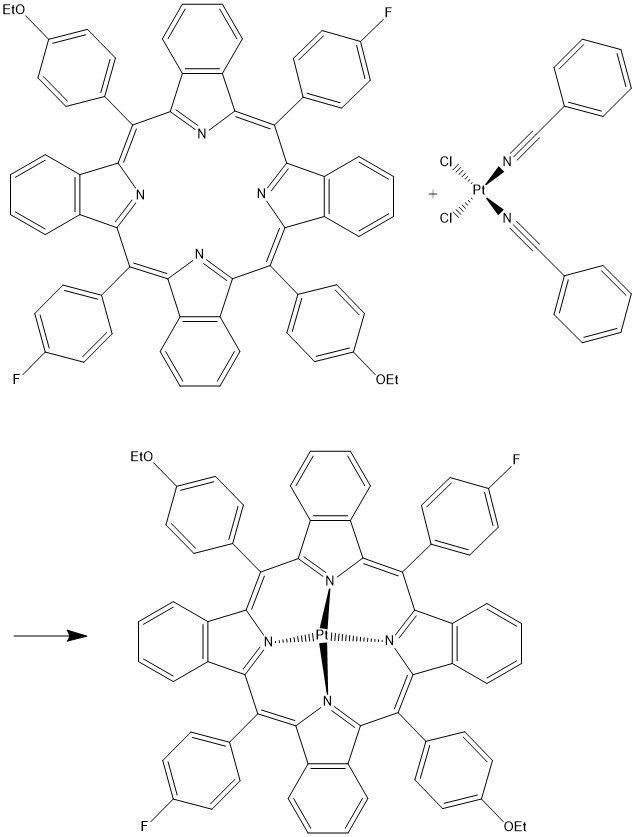
\includegraphics[scale=0.5]{graphics/Platinierung}
\end{figure}
Die Platinierung (Einführung von Platin als Zentralatom in den demetallierten Komplex) wurde durchgeführt, weil Pt-Komplexe stabiler sind und das Absorptionsspektrum nach rechts (naher Infrarotbereich) verschoben wird.
Nach der Platinierung wurde eine Säulenchromatographie zur Aufreinigung gemacht. Jedoch stellte sich laut Spektrum die Trennung der einzelnen Komponenten als schwierig heraus, da bei Aufnahme des Spektrums bei den einzelnen Fraktionen mehrere Peaks erkennbar sind. Mittels Säulenchromatographie könnte kein reines Produkt erhalten werden. Es gibt zwei Hauptpeaks bei 479 nm und bei 645 nm. Dazwischen sind kleinere Peaks zu sehen, die noch auf Nebenprodukte hindeuten. Deswegen wurde an dieser Stelle abgebrochen.

\section{Schollreaktion}
\subsection{Pt(II)tertbutylbenzoporphyrin}
\begin{figure}
\centering
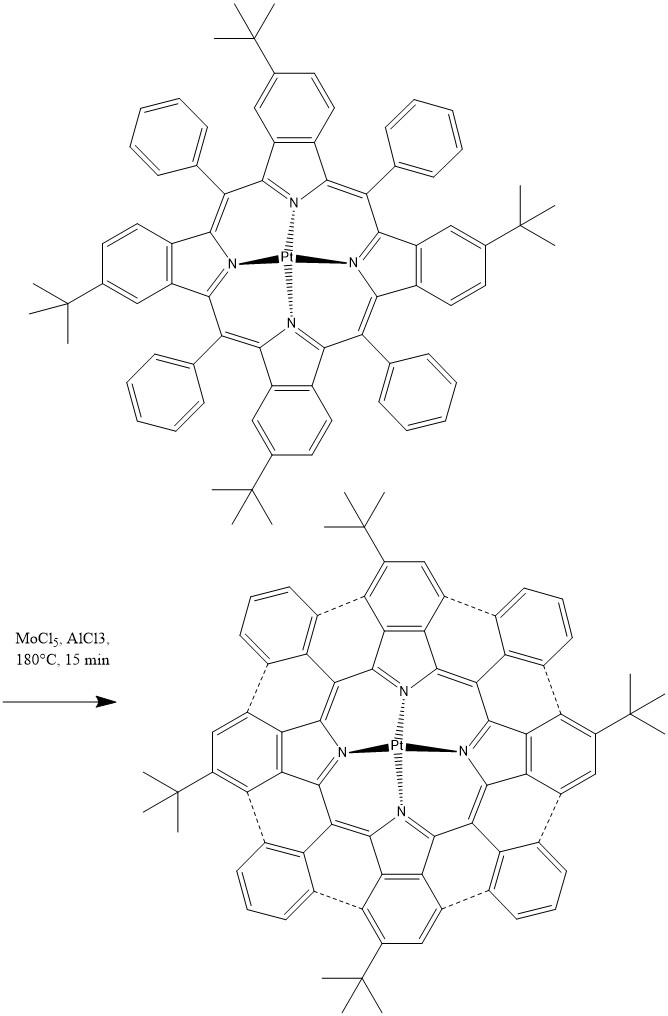
\includegraphics[scale=0.5]{graphics/PttBuTBPreaction}
Die Verbrückung erfolgte um das Spektrum des Komplexes naxh rechts zu verschieben
\end{figure}
\begin{figure}[!htpb]
\centering
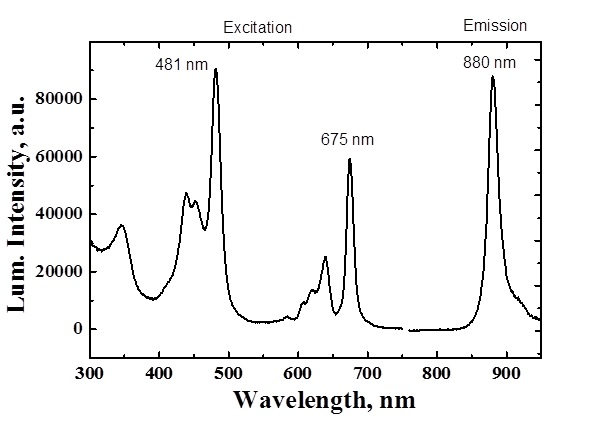
\includegraphics[scale=0.5]{graphics/PttBuTBPafterschollreaction}
\caption{Fluoreszenzspektrum von PttBuTBP nach der Schollreaktion}
\end{figure}
Die Anregung erfolgte bei 481 nm und die Emission bei 880 nm. Die Peaks bei 481 und 675 nm sind sehr spitz und ihnen gehen geringere Spitzen vorraus. Die Emission bei 880 nm weist ebenfalls einen spitzen Peak auf. Damit liegt das Emissionsspektrum im nahen Infrarot-Bereich.


\begin{figure}[!htpb]
\centering
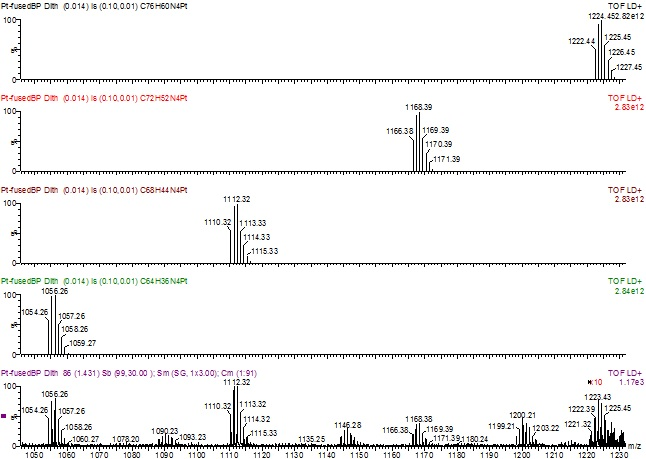
\includegraphics[scale=1]{graphics/PttBuTBPmassspktrum2}
\caption{theoretisches Massenspektrum von PttBuTBP}
\end{figure}

Im Bild sind die theoretischen Isomere der verschieden verbrückten Benzoporphyrinen zu sehen. Mit jeder Schließung eines Ringes geht auch eine Butyl-Gruppe weg.  Die Butyl-Gruppen wurden für die Löslichkeit eingebaut, aber wahrscheinlich werden sie bei hohen Temperaturen abgespalten. Von oben nach unten ist jeweils ein, zwei, drei oder vier Phenylringe komplett miteinander verbrückt sind. Das letzte Spektrum zeigt die experimentell gefundenen Massenspektren. Dabei sieht man, dass ich dreifach und vierfach verbrückte Benzoporphyrine bilden und einfach und zweifach eher nicht bilden. Es sind auch Isotope zwischen den einzelnen Massen zu erkennen.

\begin{figure}[!htpb]
\centering
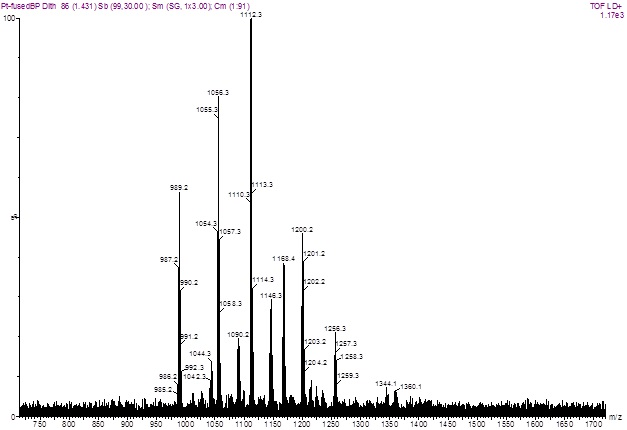
\includegraphics[scale=0.9]{graphics/PttBuTBPmassspktrum1}
\caption{Massenspektrum von PttBuTBP}
\end{figure}
Das unverbrückte Edukt hatte eine Masse von 1280 g/mol. Rechnet man jeweils 56 g/mol (tert-Butylgruppe) weg, so ergeben sich Massen von 1224, 1168, 1112 und 1056 g/mol. Diese scheinen teilweise auch im Spektrum auf. Manchmal hat sich auch ein Cl-Atom eingebaut, was Massen von 1256 und 1200 erklärt, sowie bei 1090 und 1046. Die Masse bei 989 g/mol ist unerklärlich, vermutlich wurde das Metallion entfernt.
Es haben sich mehrere Produkte mit verschieden verbrückten Phenylringen gebildet. Die Trennung dieser Produkte und die genaue Strukturanalyse wird noch eine Herausforderung in Zukunft  sein. Wenn man mit dem Porphyrin Kristallstrukturen bilden könnte, so kann die Struktur mit Röntgenstrukturanalyse herausgefunden werden. Eine Trennung und Isolierung ist vielleicht mit Säulenchromatographie möglich.
\newpage
\subsection{PttBumonoAzaTBP}
\begin{figure}[!htpb]
\centering
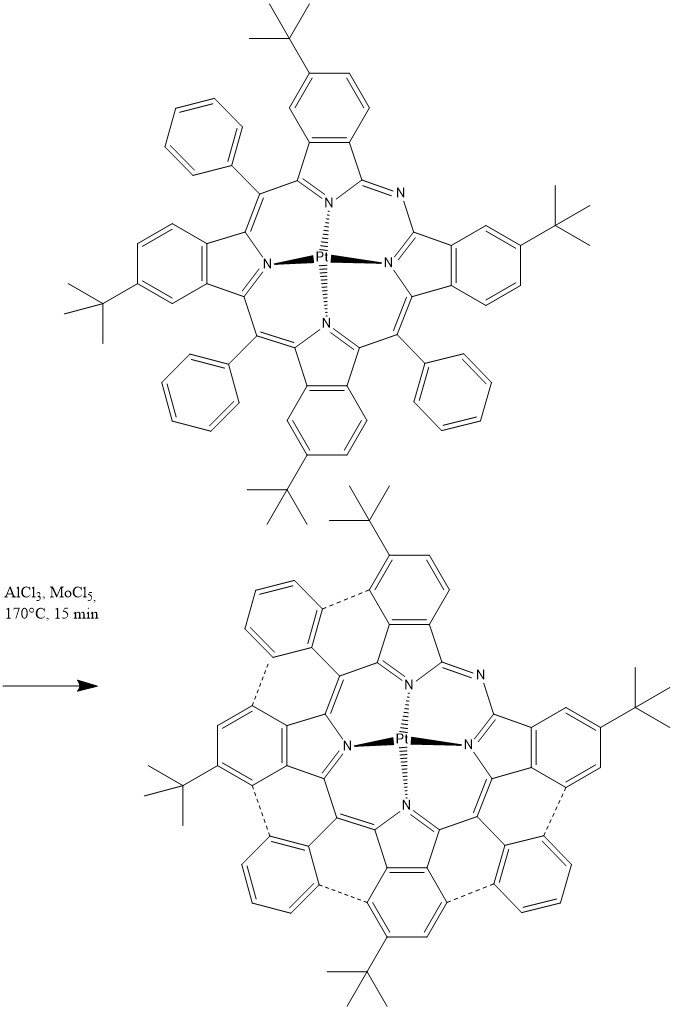
\includegraphics[scale=0.5]{graphics/PttBumonoAzaTBPreaction}
\end{figure}
Die Verbrückung erfolgte ähnlich wie beim oberen Beispiel. Das Edukt besitzt drei Phenylringe und statt eines vierten Phenylringes hat es eine Stickstoffbrücke. 

Im Fluoreszenzspektrum (\ref{Anregmononaza}) erkennt man zwischen 390 und 480 nm  einen breiten Bereich mit zwei leichten Peaks. Dieser ist undefinerter als der im vorhergehenden Beispiel. Zwischen 600 nm und 670 nm erkennt man drei Peaks, von denen der mit 660 nm der höchste und sehr spitz ist.


Die Emission (\ref{emissmonoaza}) liegt mit 925 nm im nahen Infrarot-Bereich. Es gibt nur einen Peak, der sehr spitz ist. Damit ist dieses Produkt als Indikator geeignet.
\chapter{Zusammenfassung}
Die Synthese der Porphyrine erwies sich als schwierig. Beschriebene Synthesen funktionierten nicht, weil keine stabilen Produkte gebildet werden konnten. Die Löslichkeit der Porphyrine war sehr gering, da sie große planare Strukturen bilden. Manchmal konnte man auch keine Reinigung mittels Säulenchromatographie gewährleisten.
Die gewonnene Erkenntnisse helfen aber in Zukunft, neue Strategien zu entwickeln und die besonderen Eigenschaften der Porphyrine zu berücksichtigen.
\\Sehr vielversprechend war die Verbrückung von Benzoporphyrinen mittels Schollreaktionen. Diese ergab Produkte, die im nahen Infrarotbereich emittieren und damit als Indikatoren für optische Sensoren geeignte sind. Der Einsatz eines Gemisches aus $Al_2O_3$ und MoCl$_5$ erwies sich als effektivsten. Der genaue Mechanismus dieser Reaktion ist noch nicht geklärt. Auch die genaue Struktur der verschiedene verbrückten Porphyrine muss noch erforscht werden, was im Umfang dieser Bachelorarbeit leider nicht möglich war. 
%% include tex file chapters:
% \include{introduction}        %% this is a suggestion: you have to create this file on demand
% \include{problem}             %% this is a suggestion: you have to create this file on demand
% \include{solution}            %% this is a suggestion: you have to create this file on demand
% \include{evaluation}          %% this is a suggestion: you have to create this file on demand
% \include{outlook}             %% this is a suggestion: you have to create this file on demand

\appendix                       %% closes main document, appendix follows until end; only available in book-classes
\addpart*{Appendix}             %% adding Appendix to tableofcontents
\begin{thebibliography}{99}
\bibitem{arten}
Wöhrle,D.;Tausch, M. W.; Stohrer,W. D.; \emph{Photochemie}, Wiley-VCh, 1998
\bibitem{Hesse}
Hesse, M.; Meier, H.; Zeeh, B.,
\emph{Spektroskopische Methoden in der organischen Chemie},
Georg Thieme Verlag, 2005, D-70469 Stuttgart
\bibitem{jab}
\emph{Charge-Transfer-Prozesse (Chemie)} \url{http://marjorie-wiki.de/wiki/Charge-Transfer-Prozesse_(Chemie)} ;(16.05.2014, 09:47 Uhr)
\bibitem{Valeur}
Valeur, B.,
\emph{Molecular Fluorescence}
WILEY-VCH Verlag GmbH, 2002, Weinheim
\bibitem{Schwedt}
Schwedt, G.,
\emph{Analytische Chemie; Grundlagen, Methoden und Praxis}
WILEY-VCH Verlag GmbH, 2008, Weinheim
\bibitem{Mills}
Mills,A.; Graham,A.
\emph{Extruded polymer films pigmented with a heterogeneous ion-pair based lumophore for O2 sensing}
Analyst, 2013,138, 6488-6493
\bibitem{Borisov}
Borisov, S.M.; Nuss,G.; Klimant, I.
\emph{Red Light-Excitable Oxygen Sensing Materials
Based on Platinum(II) and Palladium(II)
Benzoporphyrins}
Anal. Chem. 2008, 80, 9435–9442
\bibitem{optsensor}
Tengberg,A.;Hovdenes, J.; Barranger, D.; Brocandel, O.; Diaz, R.; Sarkkula, J.; Huber, C.; Stangelmayer, A.;
\emph{Optodes to Measure Oxygen in the
Aquatic Environment}, \url{www2.mbari.org/~coletti/dropbox/Optode/Sea_Tecnology_Feb_2003_Optodes.pdf}; (24.03.2014; 15:27 Uhr)
\bibitem{biochemie}
Buddecke, E
\emph{Grundriß der Biochemie: Für Studierende der Medizin, Zahnmedizin und Naturwissenschaften}
de Gruyter, 1994
\bibitem{arylethinylporphyrine}
Goldberg, P.K.; Pundsack, T.J.; Splan, K.E.
\emph{Photophysical Investigation of Neutral and Diprotonated Free-Base
Bis(Arylethynyl)porphyrins}
J. Phys. Chem. A 2011, 115, 10452–10460
\bibitem{Finikova}
Finikova, O.S.; Cheprakov, A.V.; Carroll, P.J.; Vinogradov; S.A.
\emph{Novel Route to Functionalized
Tetraaryltetra[2,3]naphthaloporphyrins via
Oxidative Aromatization}
J. Org. Chem. 2003, 68, 7517-7520
\bibitem{tsuda}
Tsuda, A.; Osuka, A.,
\emph{Discrete Conjugated Porphyrin Tapes
with an Exceptionally Small Bandgap}
Adv. Mater. 2002, 14, No. 1, January 4
\bibitem{schollallg.}
\emph{Scholl-Reaktion}
\url http://www.internetchemie.info/chemiewiki/index.php?title=Scholl-Reaktion (24.03.2014, 16:28)
\bibitem{Rempala}
Rempala; P.; Kroulik,J.; King, B.
\emph{Investigation of the Mechanism of the Intramolecular Scholl
Reaction of Contiguous Phenylbenzenes}
J. Org. Chem. 2006, 71, 5067-5081
\bibitem{MoCl5}
Waldvogel, S.R.; Trosien, S.,
\emph{Oxidative transformation of aryls using molybdenum pentachloride}
Chem. Commun., 2012, 48, 9109–9119
\bibitem{Lu and Moore}
Lu, Y.; Moore, J.
\emph{Semi-fused hexaphenyl hexa-peri-hexabenzocoronene: a novel fluorophore
from an intramolecular Scholl reaction}
Tetrahedron Letters 2009, 50, 4071–4077
\bibitem{Shen}
Shen, Z.; Uno, H.; Shimizu, Y.; Ono, N.;
\emph{Controlling conformations and physical properties of
meso-tetrakis(phenylethynyl)porphyrins by ring fusion: synthesis,
properties and structural characterizations}
Org.Biomol.Chem.;2004,2, 3442-3447


\end{thebibliography}
\printbibliography              %% remove, if using BibTeX instead of biblatex
% \include{further_ressources}  %% this is a suggestion: you have to create this file on demand






%%%% end{document}
\end{document}
%% vim:foldmethod=expr
%% vim:fde=getline(v\:lnum)=~'^%%%%\ .\\+'?'>1'\:'='
%%% Local Variables:
%%% mode: latex
%%% mode: auto-fill
%%% mode: flyspell
%%% eval: (ispell-change-dictionary "en_US")
%%% TeX-master: "main"
%%% End:
